Hadronic matter under conditions of extreme temperature or net baryon
density transitions to a new state of matter called the \qgp.  Lattice
QCD calculations at zero net baryon density indicate a smooth
crossover transition at $T_{c} \approx 170$~MeV, though with a rapid
change in properties at that temperature as shown in the left panel of
Figure~\ref{fig:lattice}~\cite{PhysRevD.80.014504}.  This \qgp
dominated the early universe for the first six microseconds of its
existence.  Collisions of heavy nuclei at the Relativistic Heavy Ion
Collider (RHIC) have sufficient initial kinetic energy that is then
converted into heat to create \qgp with an initial
temperature---measured via the spectrum of directly emitted
photons---of greater than 300~MeV~\cite{Adare:2008ab}. The higher
energy collisions at the Large Hadron Collider (LHC) produce an even
higher initial temperature $T > 420$~MeV~\cite{Luzum:2009sb}.

\begin{figure}[!hbt]
 \begin{center}
   \raisebox{4pt}{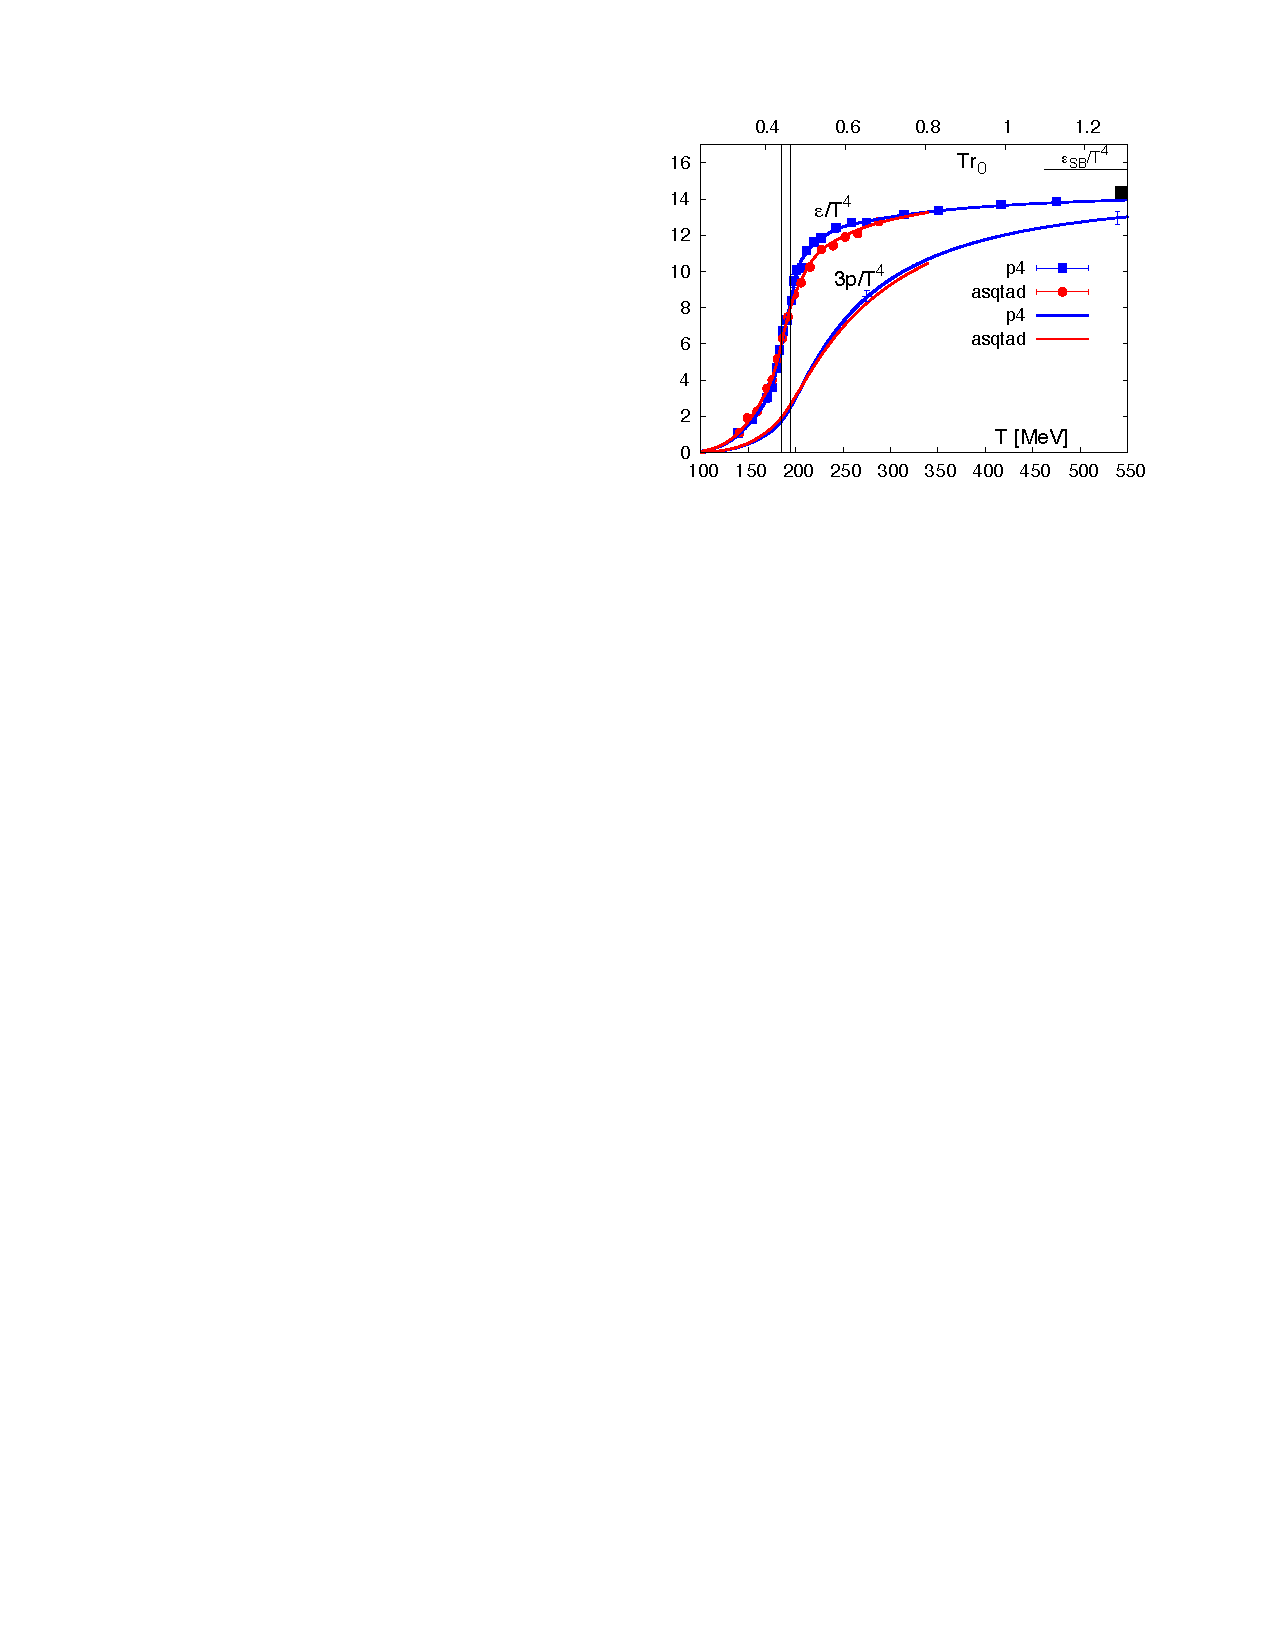
\includegraphics[trim = 2 2 2 2, clip, width=0.46\linewidth]{figs/figure_physicscase_lattice1}}
    \hfill
    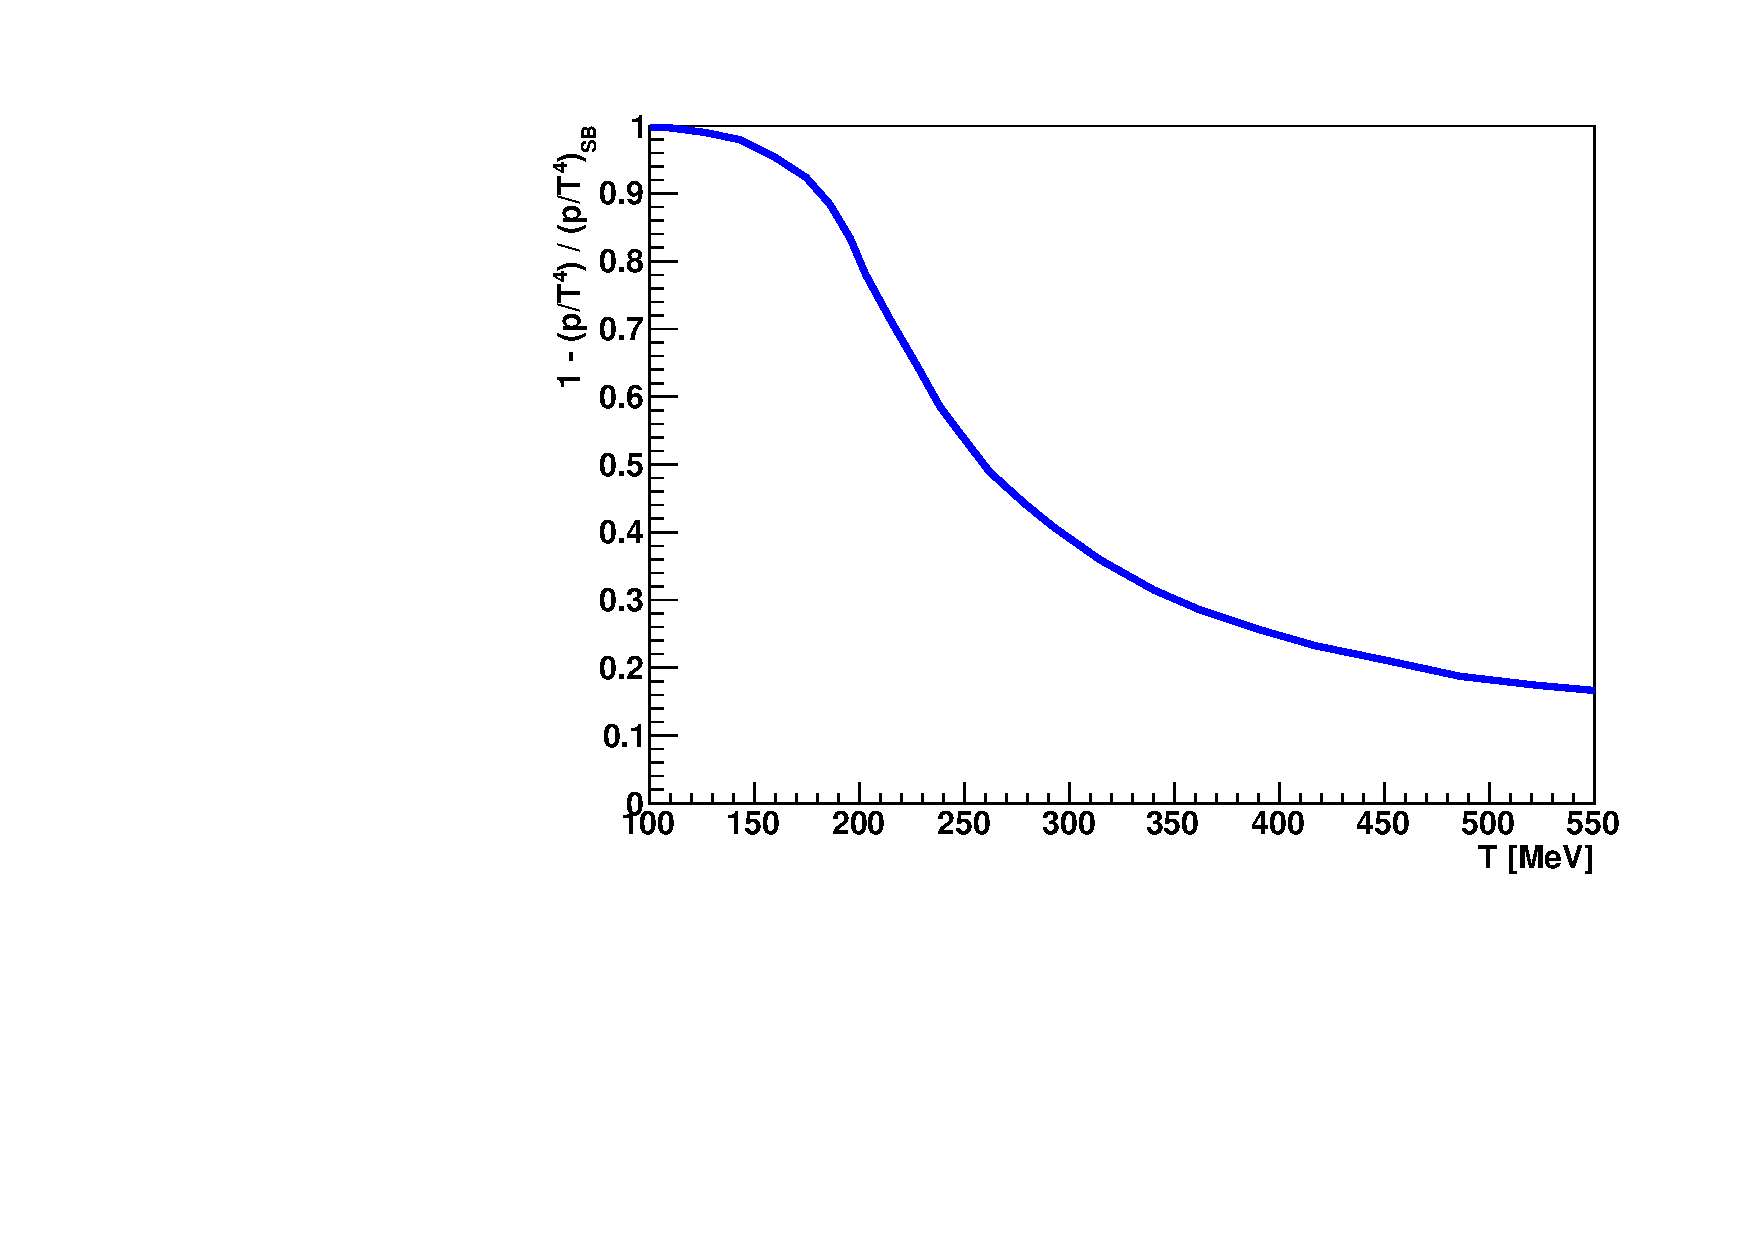
\includegraphics[trim = 2 2 2 2, clip, width=0.52\linewidth]{figs/figure_physicscase_lattice_pdev}
    \caption[$E/3p$ and $p/T^{4}$ vs temperature]{(left) The energy density and three times the pressure
      normalized by $1/T^{4}$ as a function of
      temperature~\protect\cite{PhysRevD.80.014504}{}. (right) Deviation in 
      $p/T^{4}$ relative to the Stefan-Boltzmann value as a function
      of temperature.  The deviation from the Stefan-Boltzmann value is 23\%, 39\%, 53\%, and 80\% at
      temperatures of 420, 300, 250, and 200~MeV, respectively.
    \label{fig:lattice}}
 \end{center}
\end{figure}

In materials where the dominant forces are electromagnetic, the
coupling $\alpha_{\mathrm{em}}$ is always much less than one.  Even so,
many-body collective effects can render perturbative calculations
non-convergent and result in systems with very strong
effective coupling~\cite{Adams:2012th}.  In cases where the nuclear force is
dominant, and at temperature scales of order 1--3\,$T_{c}$, the
coupling constant $\alpha_{s}$ is not much less than one and the
system is intrinsically non-perturbative.  In addition, the many-body
collective effects in the \qgp and their temperature dependence near
$T_{c}$ are not yet well understood.

INSERT FIGURE FROM NSAC LRP SIDEBAR WITH COMPARISON OF ARPES PROBES FOR HIGH TC SUPERCONDUCTORS AND SPHENIX ON QGP.   -- ONE OPTION (jln).

The right panel of Figure~\ref{fig:lattice} shows the deviation from
the Stefan-Boltzmann limit of Lattice QCD results for the pressure
normalized by $1/T^{4}$.  The Stefan-Boltzmann limit holds for a
non-interacting gas of massless particles (i.e., the extreme of the
weakly coupled limit), and as attractive inter-particle interactions
grow stronger the pressure decreases.  Thus, one might expect that the
\qgp would transition from a weakly coupled system at high temperature
to a more strongly coupled system near $T_{c}$.  However, a direct
quantitative extraction of the coupling strength warrants caution as
string theory calculations provide an example where the coupling is
very strong and yet the deviation from the Stefan-Boltzmann limit is
only 25\%~\cite{Gubser:2009fc,Gubser:1996de}.  The change in initial
temperature between RHIC and LHC collisions is thus expected to be
associated with important changes in the nature of the
\qgp~\cite{Wiedemann:2009sa}.  If not, the question is why not.

The collisions at RHIC and the LHC involve a time evolution during
which the temperature drops as the \qgp expands.  The real constraint
on the temperature dependence of the \qgp properties will come from
calculations which simultaneously describe observables measured at both energies.
Since we are studying a phase transition, it is crucial to do
experiments near the phase transition and compare them with
experiments done further above $T_c$.  Typically, all the non-scaling
behavior is found near the transition.

For many systems the change in coupling strength is related to
quasiparticle excitations or strong coherent fields, and to study
these phenomena one needs to probe the medium at a variety of length
scales.  For example, in a superconductor probed at long length
scales, one scatters from Cooper pairs; in a superconductor probed at
short distance scales one observes the individual electrons.  Hard
scattered partons generated in heavy ion collisions that traverse the
\qgp serve as the probes of the medium.  Utilizing these partonic
probes, measured as reconstructed jets, over the broadest possible
energy scale is a key part of unraveling the quasiparticle puzzle in
the \qgp.  Jets at the LHC reach the highest energies, the largest initial
virtualities, and large total energy loss to probe the shortest distance scales. The lower
underlying event activity at RHIC will push the jet probes to lower energies and lower
initial virtualities thus probing the important longer distance scales in the medium.
Measurements of the three Upsilon states that span a large range in binding energy 
and size are an excellent complement to the jet program, with precision required at 
both RHIC and the LHC.

Continued developments in techniques for jet reconstruction in the
environment of a heavy ion collision have allowed the LHC experiments
to reliably recover jets down to
40~GeV~\cite{Aad:2013sla,Aad:2012vca}, which is well within the range
of reconstructed jet energies at RHIC.  This overlap opens the
possibility of studying the \qgp at the same scale but under different
conditions of temperature and coupling strength.

Apart from the temperature and coupling strength differences in the medium created
at RHIC and the LHC, the difference in the steepness of the hard scattering \pt spectrum
plays an important role.   The less steeply falling spectrum at the LHC has the benefit
of giving the larger reach in \pt with reconstructed jets expected up to 1 TeV.   At RHIC,
the advantage of the more steeply falling spectrum is the greater sensitivity to the medium
coupling and \qgp modifications of the parton shower.   This greater sensitivity may enable
true tomography in particular with engineering selections for quarks and/or gluons with longer
path length through the medium.   In addition, for correlations, once a clean direct photon or jet
tag is made, the underlying event is 2.5 times smaller at RHIC compared to the LHC thus giving
cleaner access to the low energy remnants of the parton shower and possible medium response.

This Chapter is organized into Sections as follows.  We first describe
the key ways of 'pushing' and 'probing' the \qgp to understand its
properties.  We then discuss three different aspects in which the RHIC
jet results are crucial in terms of (1) the temperature dependence of
the QGP, (2) the microscopic inner workings of the QGP, and (3) the
QGP time evolution along with the parton shower evolution.  We relate each
of these three aspects to specific observables measurable with sPHENIX.  We then
discuss the current state of jet probe measurements from RHIC and LHC
experiments, followed by a review of theoretical calculations for RHIC
jet observables.  We discuss the specific physics of heavy quark jets and open
heavy flavor in terms of Upsilon observables.   Finally, we review the rates available
that enable precision measurements across this comprehensive program.

\section{Probing the QGP acrosss length scales}

Results from RHIC and LHC heavy ion experiments have provided a wealth
of data for understanding the physics of the \qgp.  One very
surprising result discovered at RHIC was the fluid-like flow of the
\qgp~\cite{Adcox:2004mh}, in stark contrast to some expectations that
the \qgp would behave as a weakly coupled gas of quarks and gluons.
It was originally thought that even at temperatures as low as
2--5\,$T_{c}$, the \qgp could be described with a weakly coupled
perturbative approach despite being quite far from energy scales
typically associated with asymptotic freedom.  

The \qgp created in heavy ion collisions expands and cools, eventually passing through the
phase transition to a state of hadrons, which are then measured by
experiment.  Extensive measurements of the radial and flow coefficients of
various hadrons, when compared to hydrodynamics calculations, imply a very
small ratio of shear viscosity to entropy density,
$\eta/s$~\cite{Luzum:2008cw}.  In the limit of very weak coupling
(i.e., a non-interacting gas), the shear viscosity is quite large as
particles can easily diffuse across a velocity gradient in the medium.
Stronger inter-particle interactions inhibit diffusion to the limit
where the strongest interactions result in a very short mean free path
and thus almost no momentum transfer across a velocity gradient,
resulting in almost no shear viscosity.  

The shortest possible mean
free path is of order the de~Broglie wavelength, which sets a lower
limit on $\eta/s$~\cite{Danielewicz:1984ww}.  A more rigorous
derivation of the limit $\eta/s \ge 1/4\pi$ has been calculated
within string theory for a broad class of strongly coupled gauge
theories by Kovtun, Son, and Starinets (KSS)~\cite{Kovtun:2004de}.
Viscous hydrodynamic calculations assuming $\eta/s$ to be temperature
independent through the heavy ion collision time evolution are
consistent with the experimental data where $\eta/s$ is within 50\% of
this lower bound for strongly coupled
matter~\cite{Luzum:2008cw,Song:2007ux,Alver:2010dn,Teaney:2009qa,Schenke:2011zz,Adare:2011tg}.
Even heavy quarks (i.e., charm and beauty) are swept up in the fluid
flow and theoretical extractions of the implied $\eta/s$ are equally
small~\cite{Adare:2006nq}.

%\begin{figure}[t]
% \begin{center}
%   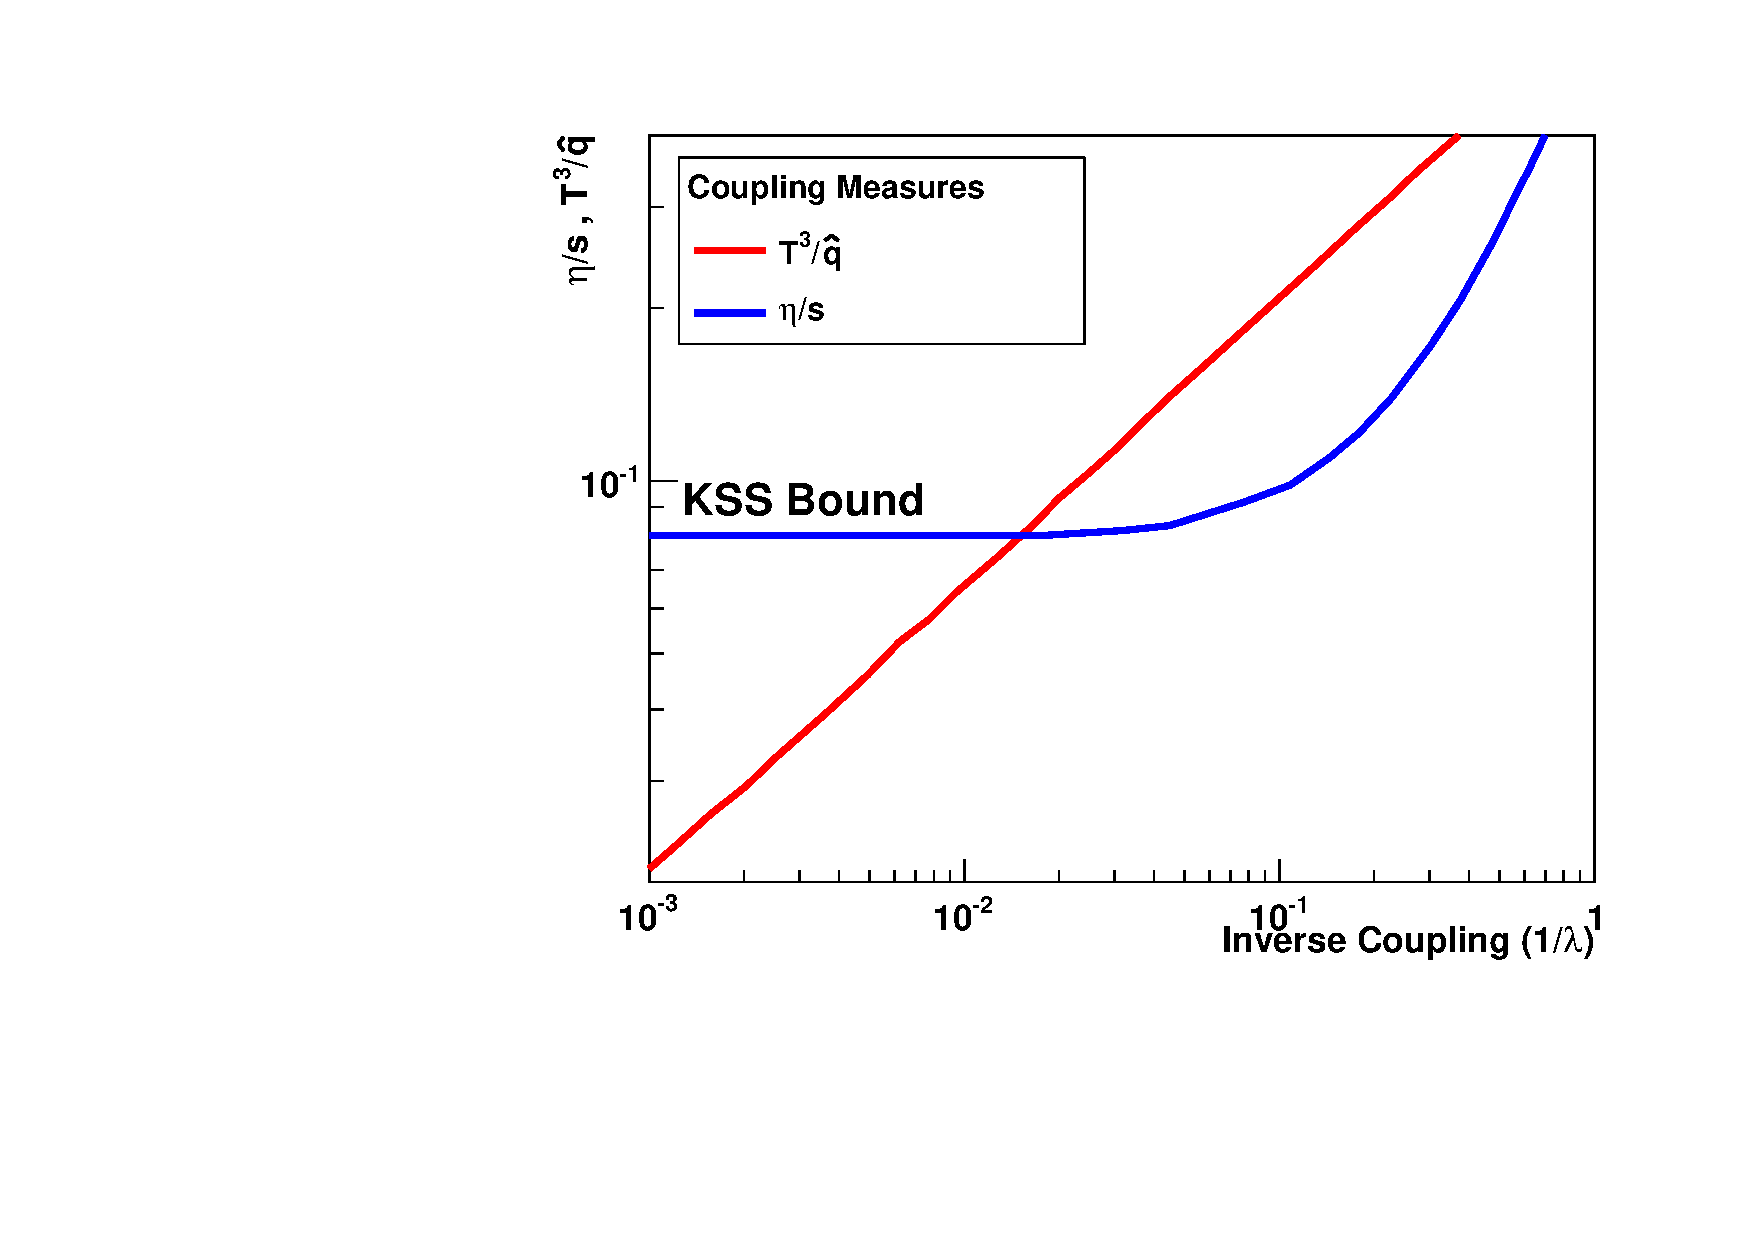
\includegraphics[width=\onewidth]{figs/etas_qhat_plot} 
%   \caption[$\eta/s$ and $T^3/\hat{q}$ vs inverse 't~Hooft coupling]{
%     $\eta/s$ (blue) and $T^3/\hat{q}$ (red) as a function of the
%     inverse of the 't~Hooft coupling\protect\cite{Majumder:2007zh}{}.
%     For large $\lambda$ (i.e., small $1/\lambda$), $\eta/s$
%     approaches the quantum lower bound asymptotically, losing its
%     sensitivity to further changes in the coupling strength.}
%    \label{fig:etas_versus_qhat} 
% \end{center}
%\end{figure}

%Other key measures of the coupling strength to the medium are found in
%the passage of a hard scattered parton through the \qgp.  As the
%parton traverses the medium it accumulates transverse momentum as
%characterized by $\hat{q} = d(\Delta p_{T}^{2})/dt$ and transfers
%energy to the medium via collisions as characterized by $\hat{e} =
%dE/dt$.  

%Ref.~\cite{Liu:2006ug} has calculated $\hat{q}/T^3$ in
%${\cal N} = 4$ supersymmetric Yang-Mills theory to be proportional to
%the square root of the coupling strength whereas $\eta/s$
%asymptotically approaches the quantum lower bound as the coupling
%increases.  Both of these ratios are shown as a function of the
%inverse coupling in Figure~\ref{fig:etas_versus_qhat}.  For large 't
%Hooft coupling ($\lambda$), $\eta/s$ is already quite close to
%$1/4\pi$, whereas $T^3/\hat{q}$ is still changing.  This behavior has
%caused the authors of Ref.~\cite{Majumder:2007zh} to comment: ``The
%ratio $T^{3}/\hat{q}$ is a more broadly valid measure of the coupling
%strength of the medium than $\eta/s$.''

In vacuum, the hard scattered parton creates a shower of particles
that eventually form a cone of hadrons, referred to as a jet.  In the
\qgp, the lower energy portion of the shower may eventually be
equilibrated into the medium, thus giving a window on the rapid
thermalization process in heavy ion collisions.  This highlights part
of the reason for needing to measure the fully reconstructed jet
energy and the correlated particle emission with respect to the jet at
all energy scales.  In particular, coupling parameters such as
$\hat{q}$ and $\hat{e}$ are scale dependent and must take on weak
coupling values at high enough energies and strong
coupling values at thermal energies.

\begin{figure}[ht]
 \begin{center}
   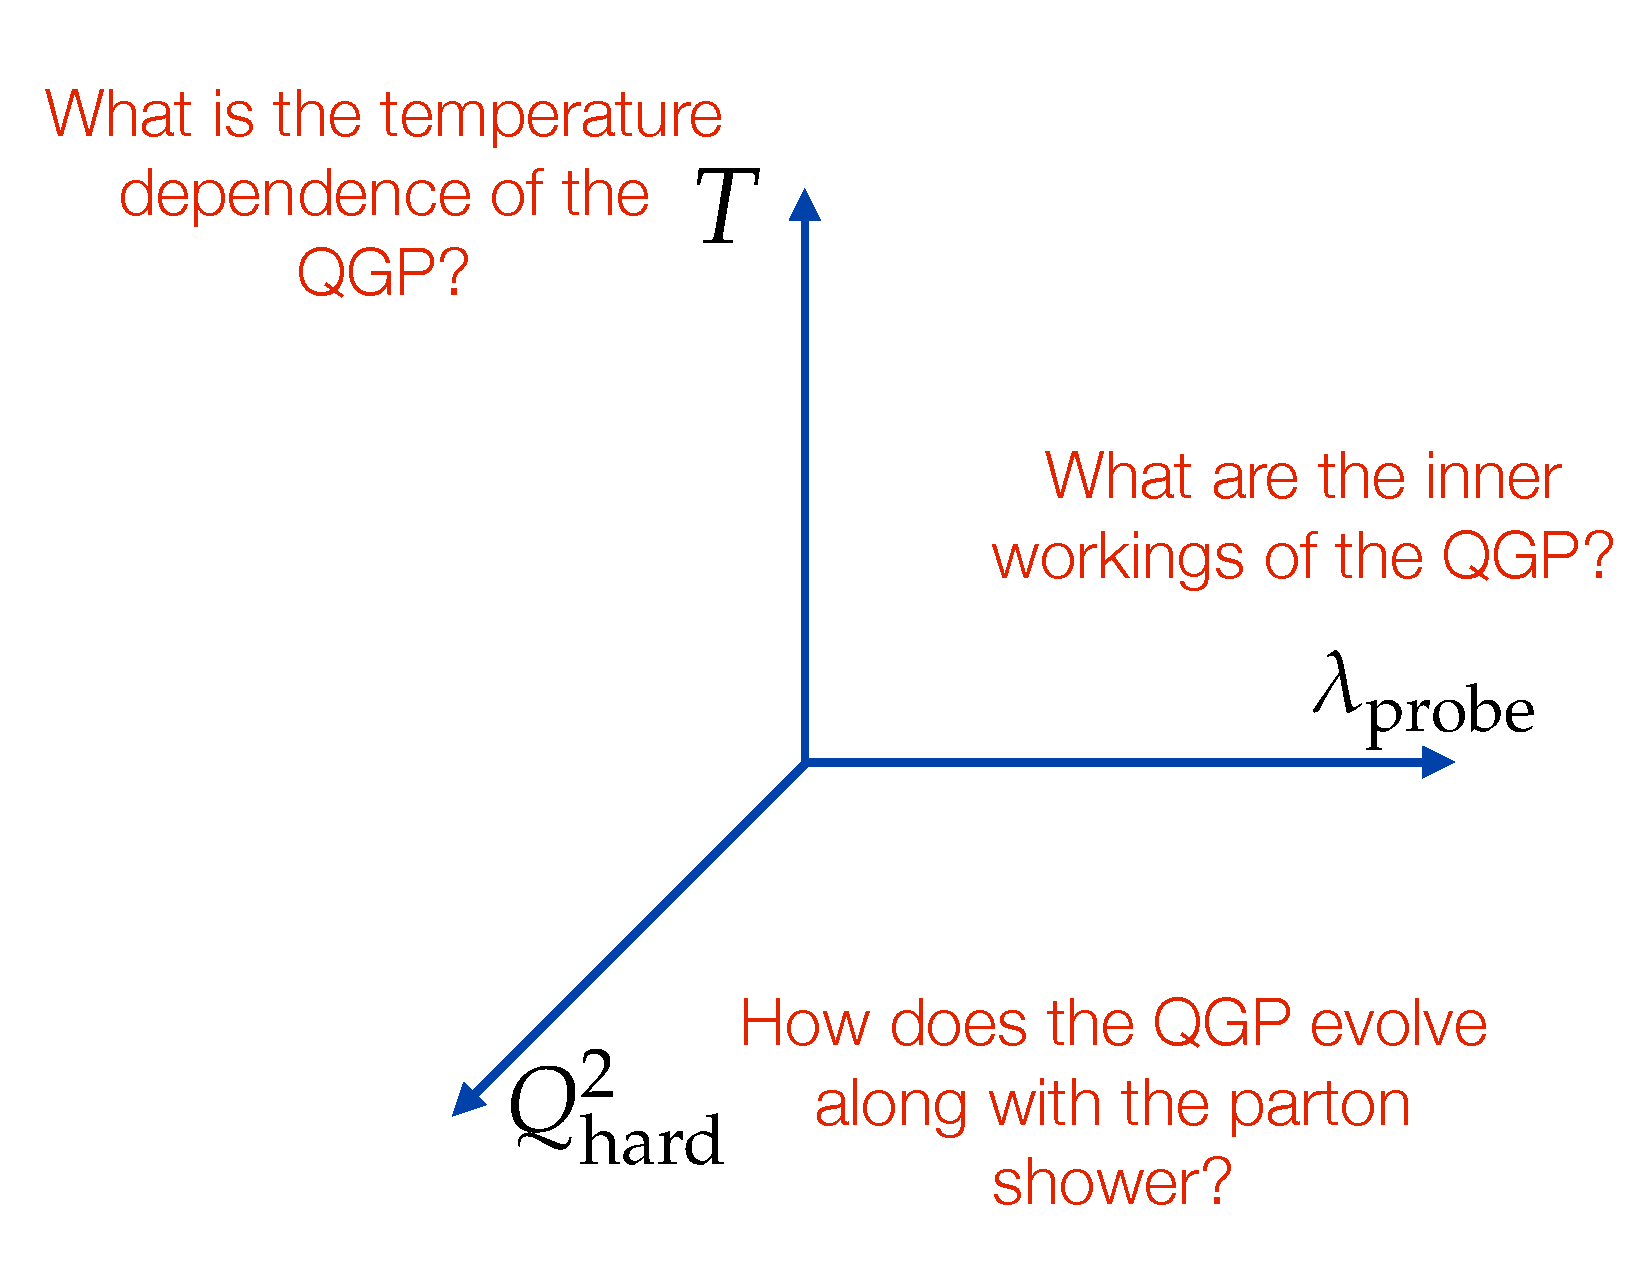
\includegraphics[trim = 2 2 2 2, clip, width=\onewidth]{figs/figure_physicscase_threeaxes}
   \caption[ Pushing and probing the \qgp along three axes]{Pushing
     Three illustrative axes along which the \qgp may be pushed and
     probed.  The axes are the temperature of the \qgp, the
     $Q^2_{\mathrm{hard}}$ of the hard process that sets of the scale
     for the virtuality evolution of the probe, and the wavelength
     with which the parton probes the medium
     $\lambda_{\mathrm{probe}}$.}
   \label{fig:threeaxes}
 \end{center}
\end{figure}

The focus of this proposal is the measurement of jet probes of the
medium as a way of understanding the coupling of the medium, the
origin of this coupling, and the mechanism of rapid equilibration.
%Some of these jet probe measurements are already being carried out by the LHC experiments.  
The \qgp is one form of the ``condensed matter''
of QCD and in any rigorous investigation of condensed matter of any
type, it is critical to make measurements as one pushes the system
closer to and further from a phase transition and with probes at
different length scales.  
Substantially extending these scales with measurements at RHIC, particularly closer 
to the transition temperature and at longer distance scales, is the unique ability provided by this proposal.

%Substantially extending these scales, 
%particularly closer to the transition temperature and at longer
%distance scales, is the unique ability of this proposal with
%measurements at RHIC.

The critical variables to manipulate for this program are the temperature of
the \qgp, the length scale probed in the medium, and the virtuality of
the hard process as shown schematically in Figure~\ref{fig:threeaxes}.
In the following three sections we detail the physics of each axis.

\section{What is the temperature dependence of the QGP?}
\label{sec:temperature_dependence}

The internal dynamics of more familiar substances---the subjects of
study in conventional condensed matter and material physics---are
governed by quantum electrodynamics.  It is well known that near a
phase boundary they demonstrate interesting behaviors, such as the
rapid change in the shear viscosity to entropy density ratio,
$\eta/s$, near the critical temperature, $T_c$. This is shown in
Figure~\ref{fig:etaovers_1} for water, nitrogen, and
helium~\cite{Csernai:2006zz}.  Despite the eventual transition to
superfluidity at temperatures below $T_{c}$, $\eta/s$ for these
materials remains an order of magnitude above the conjectured quantum
bound of Kovtun, Son, and Starinets (KSS) derived from string
theory~\cite{Kovtun:2004de}.  These observations provide a deeper
understanding of the nature of these materials: for example the
coupling between the fundamental constituents, the degree to which a
description in terms of quasiparticles is important, and the
description in terms of normal and superfluid components.

\begin{figure}[t]
 \begin{center}
    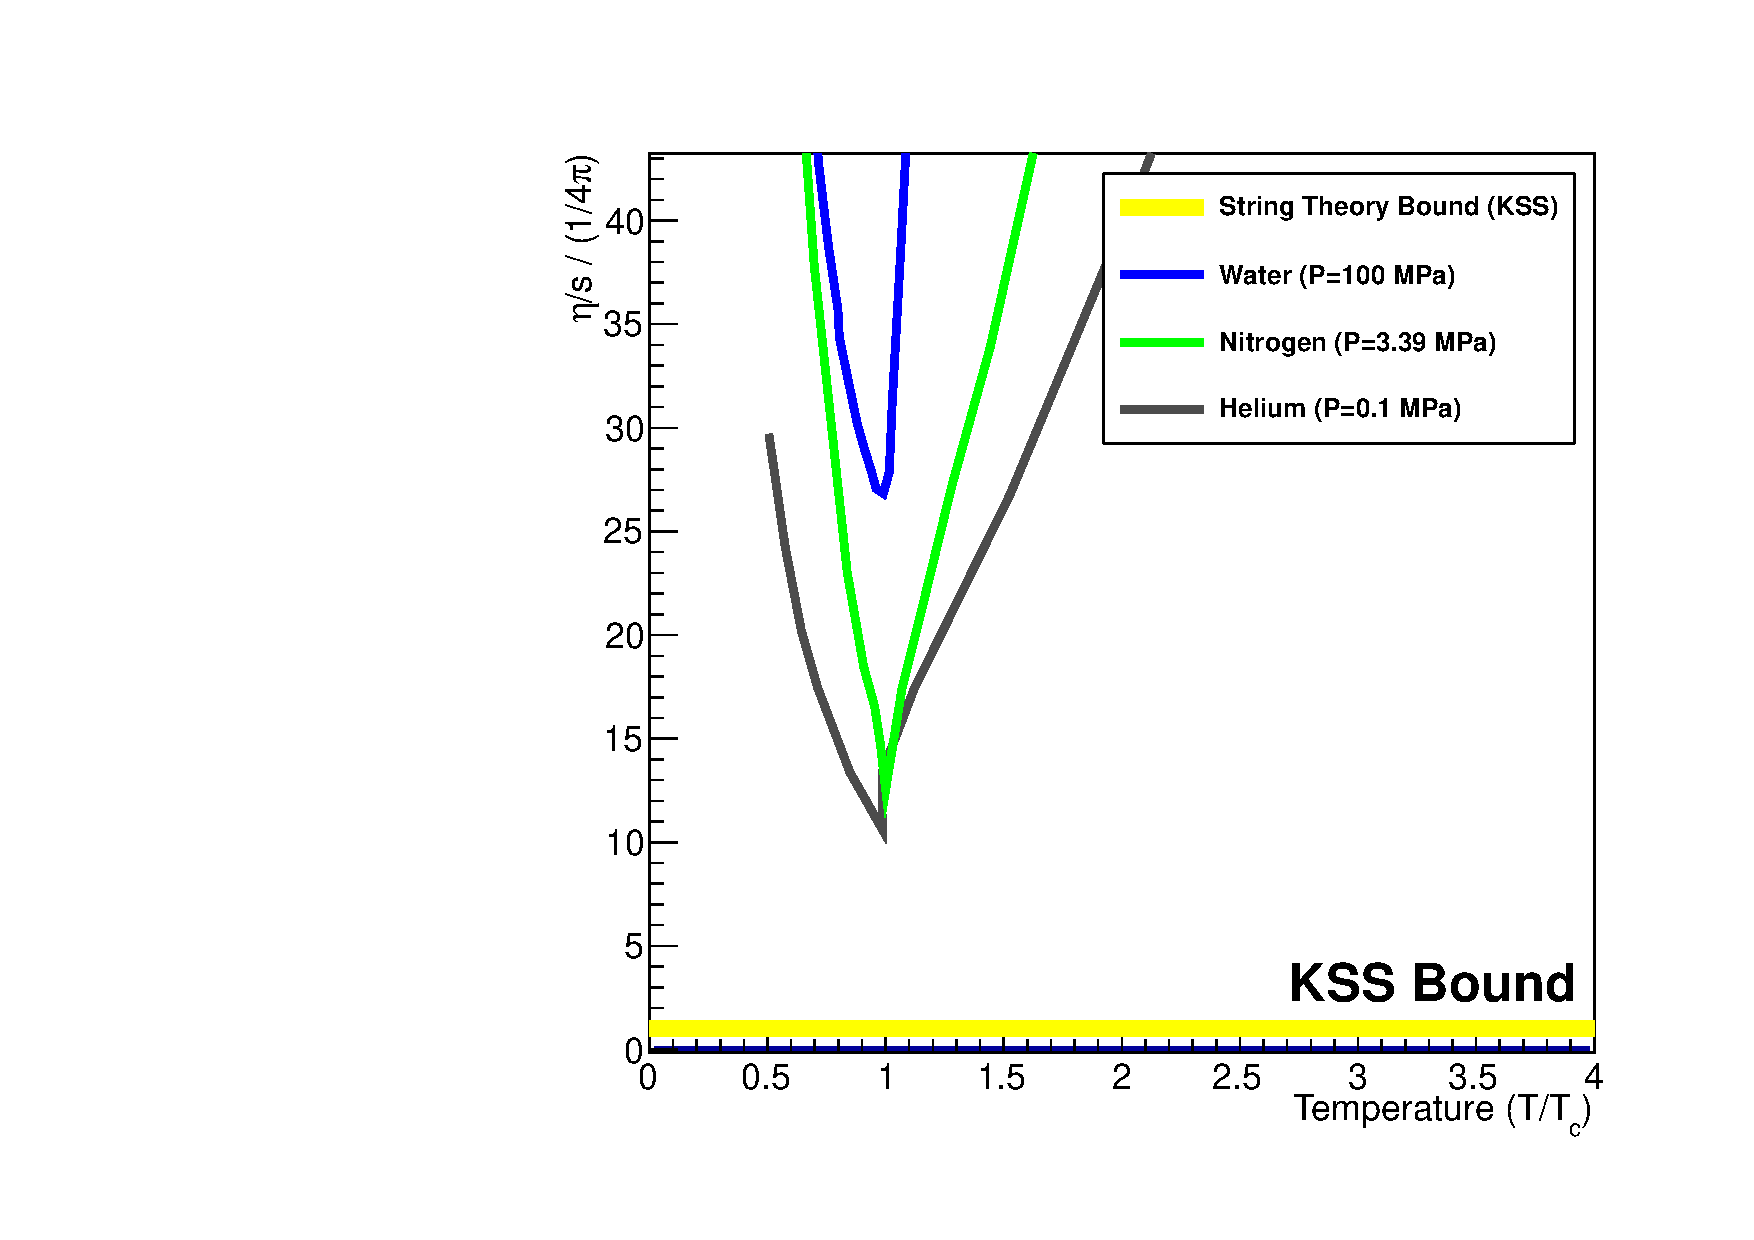
\includegraphics[trim = 2 2 2 2, clip, width=\twowidth]{figs/figure_physicscase_etaovers_liquids}
    \hfill
    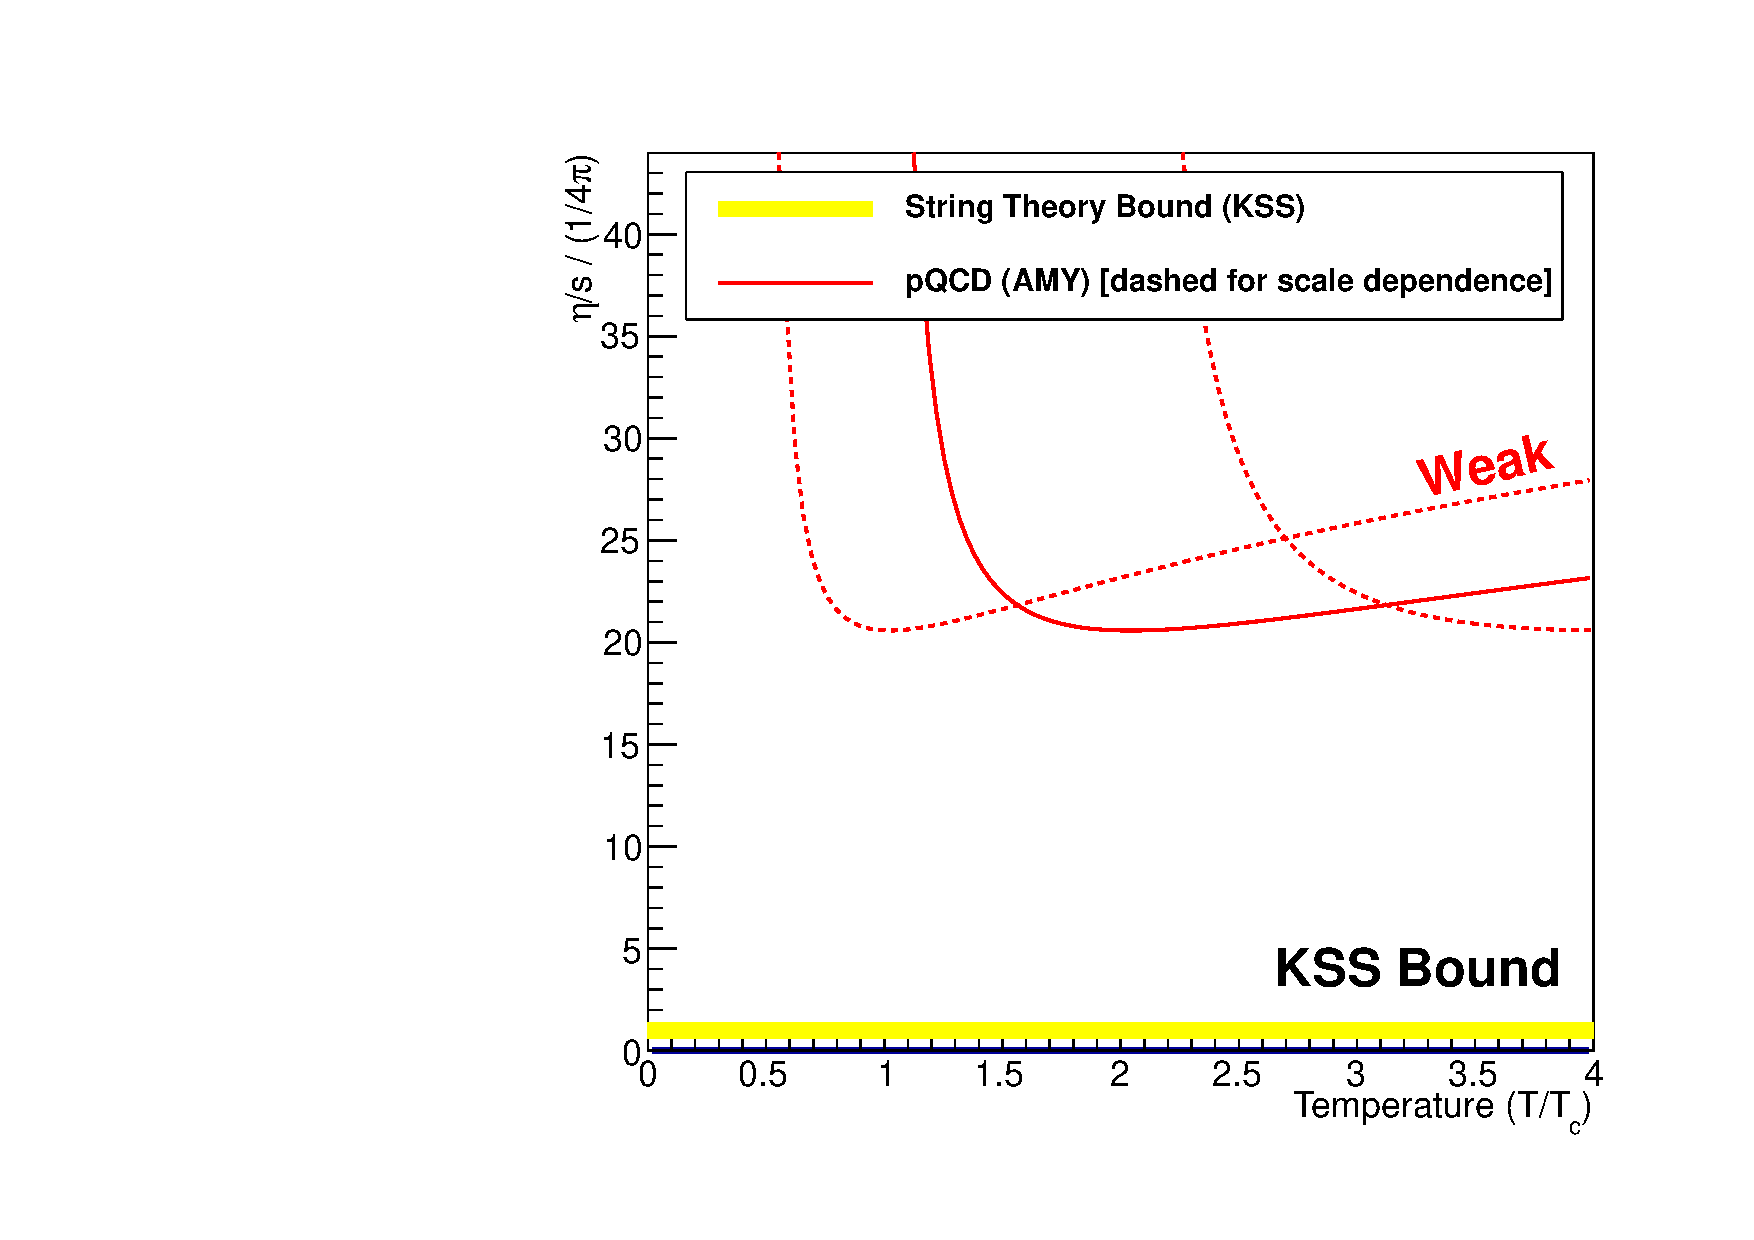
\includegraphics[trim = 2 2 2 2, clip, width=\twowidth]{figs/figure_physicscase_etaovers_qgpweak}
    \caption[$\eta/s$ vs $T/T_{c}$ for water, nitrogen, and
    helium]{(left) The ratio of shear viscosity to entropy density,
      $\eta/s$, normalized by the conjectured KSS bound as a function
      of the reduced temperature, $T/T_{c}$, for water, nitrogen, and
      helium. The cusp for Helium corresponds to the case at the
      critical pressure.  (right) Calculation of hot QCD matter
      (quark-gluon plasma) for a weakly coupled system.  Dashed lines
      show the scale dependence of the perturbative calculation.}
    \label{fig:etaovers_1}
 \end{center}
\end{figure}

The dynamics of the QGP are dominated by Quantum Chromodynamics and the
experimental characterization of the dependence of $\eta/s$ on
temperature will lead to a deeper understanding of strongly coupled
QCD near this fundamental phase transition.  Theoretically,
perturbative calculations in the weakly coupled limit indicate that
$\eta/s$ decreases slowly as one approaches $T_{c}$ from above, but
with a minimum still a factor of 20 above the KSS
bound~\cite{Arnold:2003zc}.

%(as shown in the right panel of
%Figure~\ref{fig:etaovers_1}).  However, as indicated by the dashed
%lines in the figure, the perturbative calculation has a large
%renormalization scale dependence and results for different values of
%the scale parameter ($\mu, \mu/2, 2\mu$) diverge from each other near
%$T_{c}$.

%Figure~\ref{fig:etaovers_2} (left panel) shows several
%state-of-the-art calculations for $\eta/s$ as a function of
%temperature. Hadron gas calculations show a steep increase in $\eta/s$
%below $T_c$~\cite{Prakash:1993bt}, and similar results using the UrQMD
%model have also been obtained~\cite{Demir:2008tr}.  Above $T_c$ there
%is a lattice calculation in the SU(3) pure gauge
%theory~\cite{Meyer:2007ic} resulting in a value near the KSS bound at
%$T=1.65\,T_c$.  Calculations in the semi-QGP
%model~\cite{Hidaka:2009ma}, in which color is not completely ionized,
%have a factor of five increase in $\eta/s$ in the region of
%1--2\,$T_c$.  Also shown are calculations from a quasiparticle model
%(QPM) with finite $\mu_B$~\cite{Srivastava:2012sb} indicating little
%change in $\eta/s$ up to 2\,$T_c$.  There is also an update on the
%lower limit on $\eta/s$ from second order relativistic viscous
%hydrodynamics~\cite{Kovtun:2011np}, with values remaining near
%$1/4\pi$.  It is safe to say that little is known in a theoretically
%reliable way about the nature of this transition or the approach to
%weak-coupling.

Hydrodynamic modeling of the bulk medium does provide constraints on
$\eta/s$, and recent work has been done to understand the combined
constraints on $\eta/s$ as a function of temperature utilizing both
RHIC and LHC flow data sets~\cite{Gale:2012rq,Song:2011qa,Nagle:2011uz,Niemi:2011ix} and result
in values near the KSS bound around $T_c$.  

%The results from~\cite{Niemi:2011ix} as
%constrained by RHIC and LHC data on hadron transverse momentum spectra
%and elliptic flow are shown in Figure~\ref{fig:etaovers_2}. 

%These reach the pQCD weak coupled value at $20 \times 1/4\pi$
%for $T = 3.4 T_{c}$.  Also shown are two scenarios, labeled ``Song-a''
%and ``Song-b'', for $\eta/s(T)$ in ~\cite{Song:2011qa} from which the 
%authors conclude that ``one cannot unambiguously determine the
%functional form of $\eta/s(T)$ and whether the QGP fluid is more
%viscous or more perfect at LHC energy.''

%Shown in Figure~\ref{fig:etaovers_2} (right panel) are three possible
%scenarios for a more or less rapid modification of the medium from the
%strong to the weak coupling limit.  Scenario I has the most rapid
%change in $\eta/s(T)$ following the ``Song-a'' parametrization and
%Scenario III has the least rapid change going through the lattice QCD
%pure glue result~\cite{Meyer:2007ic}.  It is imperative to map out
%this region in the `condensed matter' physics of QCD and extract the
%underlying reason for the change.

%\begin{figure}[tp]
% \begin{center}
%    \includegraphics[trim = 2 2 2 2, clip, width=\twowidth]%{figs/figure_physicscase_etaovers_qgpcalcs}
%    \hfill
%    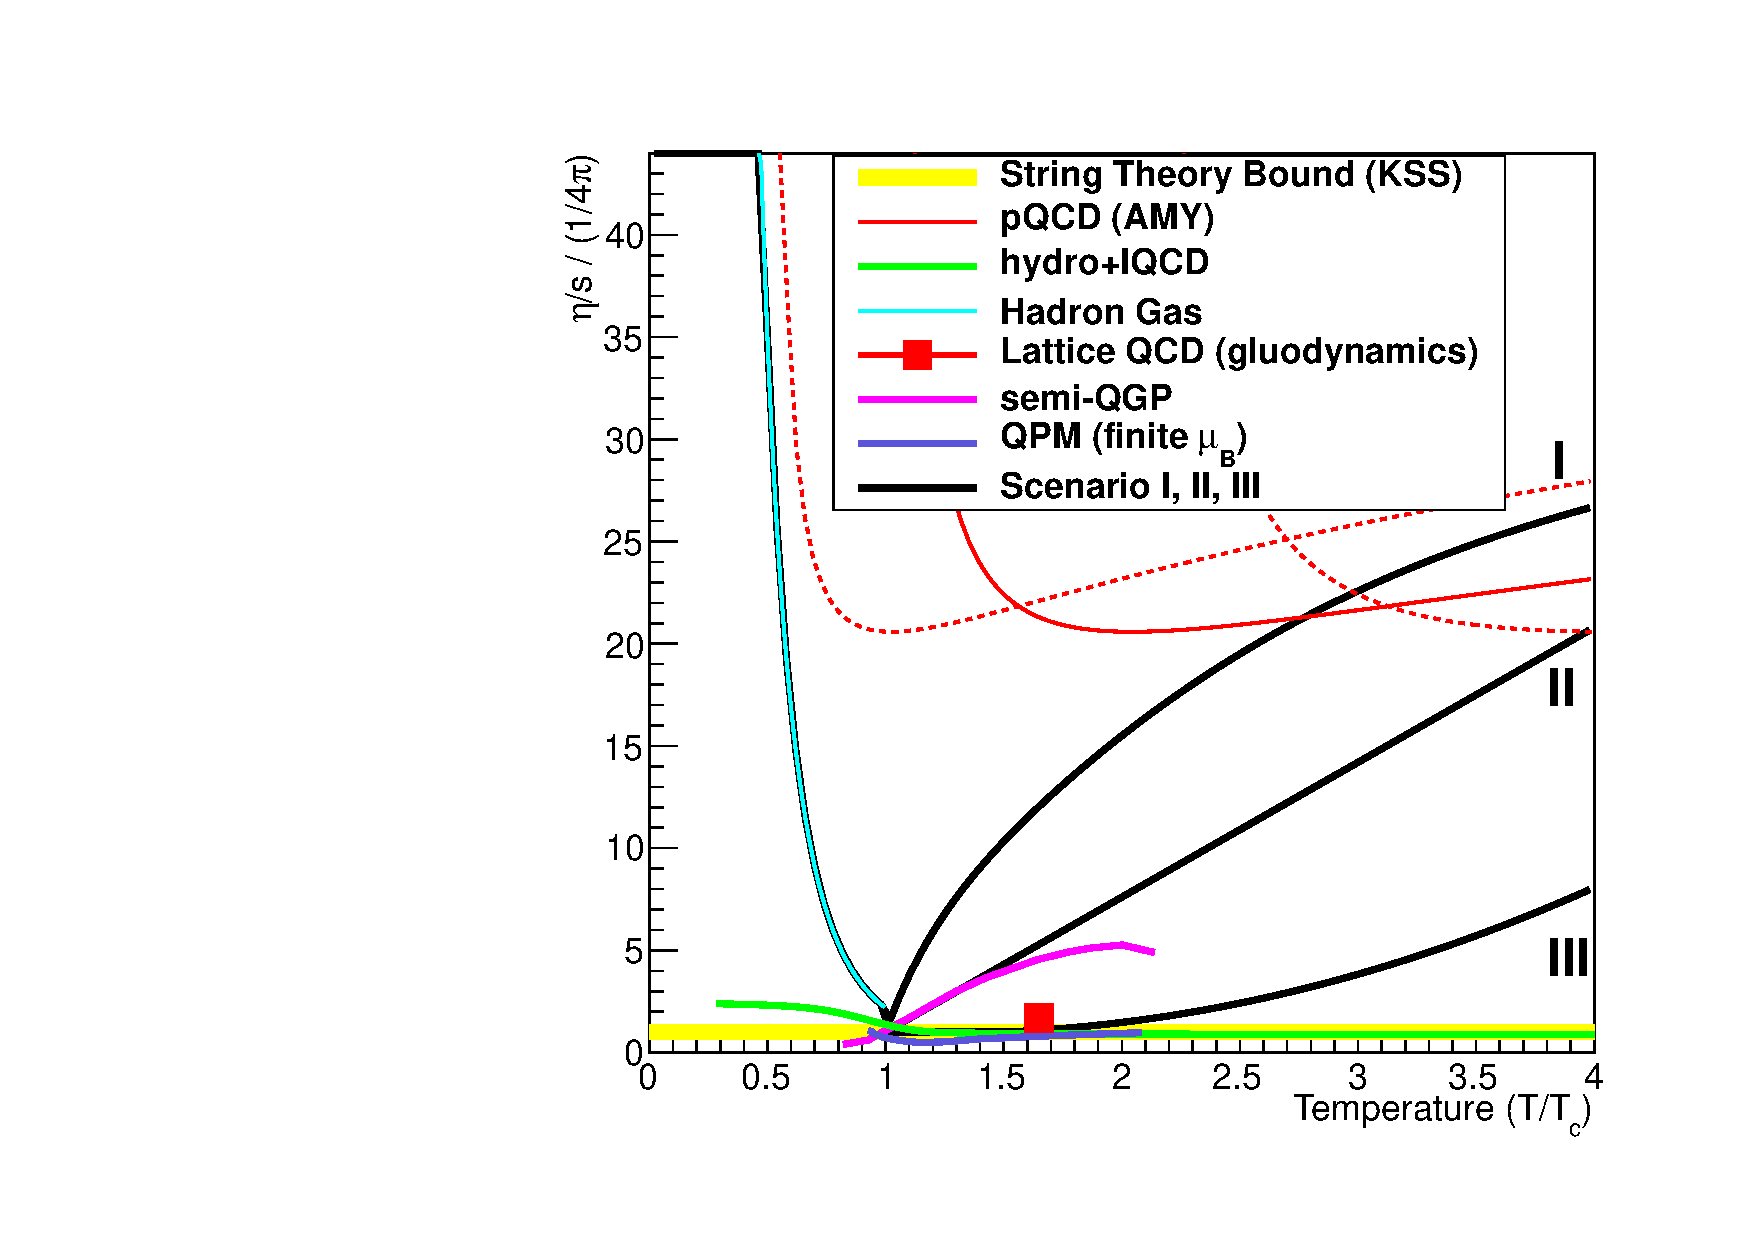
\includegraphics[trim = 2 2 2 2, clip, width=\twowidth]{figs/figure_physicscase_etaovers_qgpscenarios_modscen1}
%    \caption[ $\eta/s$ vs $T/T_{c}$ for various \qgp
%    calculations]{\label{fig:etaovers_2}(left) Shear viscosity divided
%      by entropy density, $\eta/s$, renormalized by the conjectured
%      KSS bound as a function of the reduced temperature, $T/T_{c}$,
%      with various calculations for the quark-gluon plasma case. See
%      text for discussion.  (right) Figure with three conjectured
%      scenarios for the quark-gluon plasma transitioning from the
%      strongly coupled bound (as a near-perfect fluid) to the weakly
%      coupled case.}
% \end{center}
%\end{figure}

The above discussion has focused on $\eta/s$ as the measure of the
coupling strength of the \qgp.  However, both $\eta/s$ and jet probe
parameters such as $\hat{q}$ and $\hat{e}$ are sensitive to the
underlying coupling of the matter, but in distinct ways. Establishing
for example the behavior of $\hat{q}$ around the critical temperature
is therefore essential to a deep understanding of the quark-gluon
plasma.  Hydrodynamic modeling may eventually constrain $\eta/s(T)$
very precisely, though it will not provide an answer to the question
of the microscopic origin of the strong coupling (something naturally
available with jet probes).

%However, another key handle on the
%strength of the coupling is through direct measurements of jet
%quenching, and these also give a unique insight into the structure of
%the medium itself (something not possible with hydrodynamics except
%indirectly through the equation of state).  

%The authors of Ref~\cite{Majumder:2007zh} propose a test of the strong
%coupling hypothesis by measuring both $\eta/s$ and $\hat{q}$.  They
%derive a relation between the two quantities expected to hold in the
%weak coupling limit:
%\begin{equation}
%\hat{q} \stackrel{?}{=} \frac{1.25 T^{3}}{\eta/s}.
%\label{eq:qhat2etas}
%\end{equation}
%The authors conclude that ``an unambiguous determination of both sides
%of [the equation] from experimental data would thus permit a model
%independent, quantitative assessment of the strongly coupled nature of
%the quark-gluon plasma produced in heavy ion collisions.''  For the
%three scenarios of $\eta/s(T)$ shown in Figure~\ref{fig:etaovers_2}
%(right panel), we calculate $\hat{q}$ as a function of temperature
%assuming the equivalence case in Eqn.~\ref{eq:qhat2etas} and the
%result is shown in Figure~\ref{fig:qhatmap} (left panel).  The inset in
%Figure~\ref{fig:qhatmap} shows a magnified view of the region around
%$T_c$ and a significant local maximum in $\hat{q}$ is observed in
%scenarios I and II.

%\begin{figure}[tp]
% \begin{center}
%    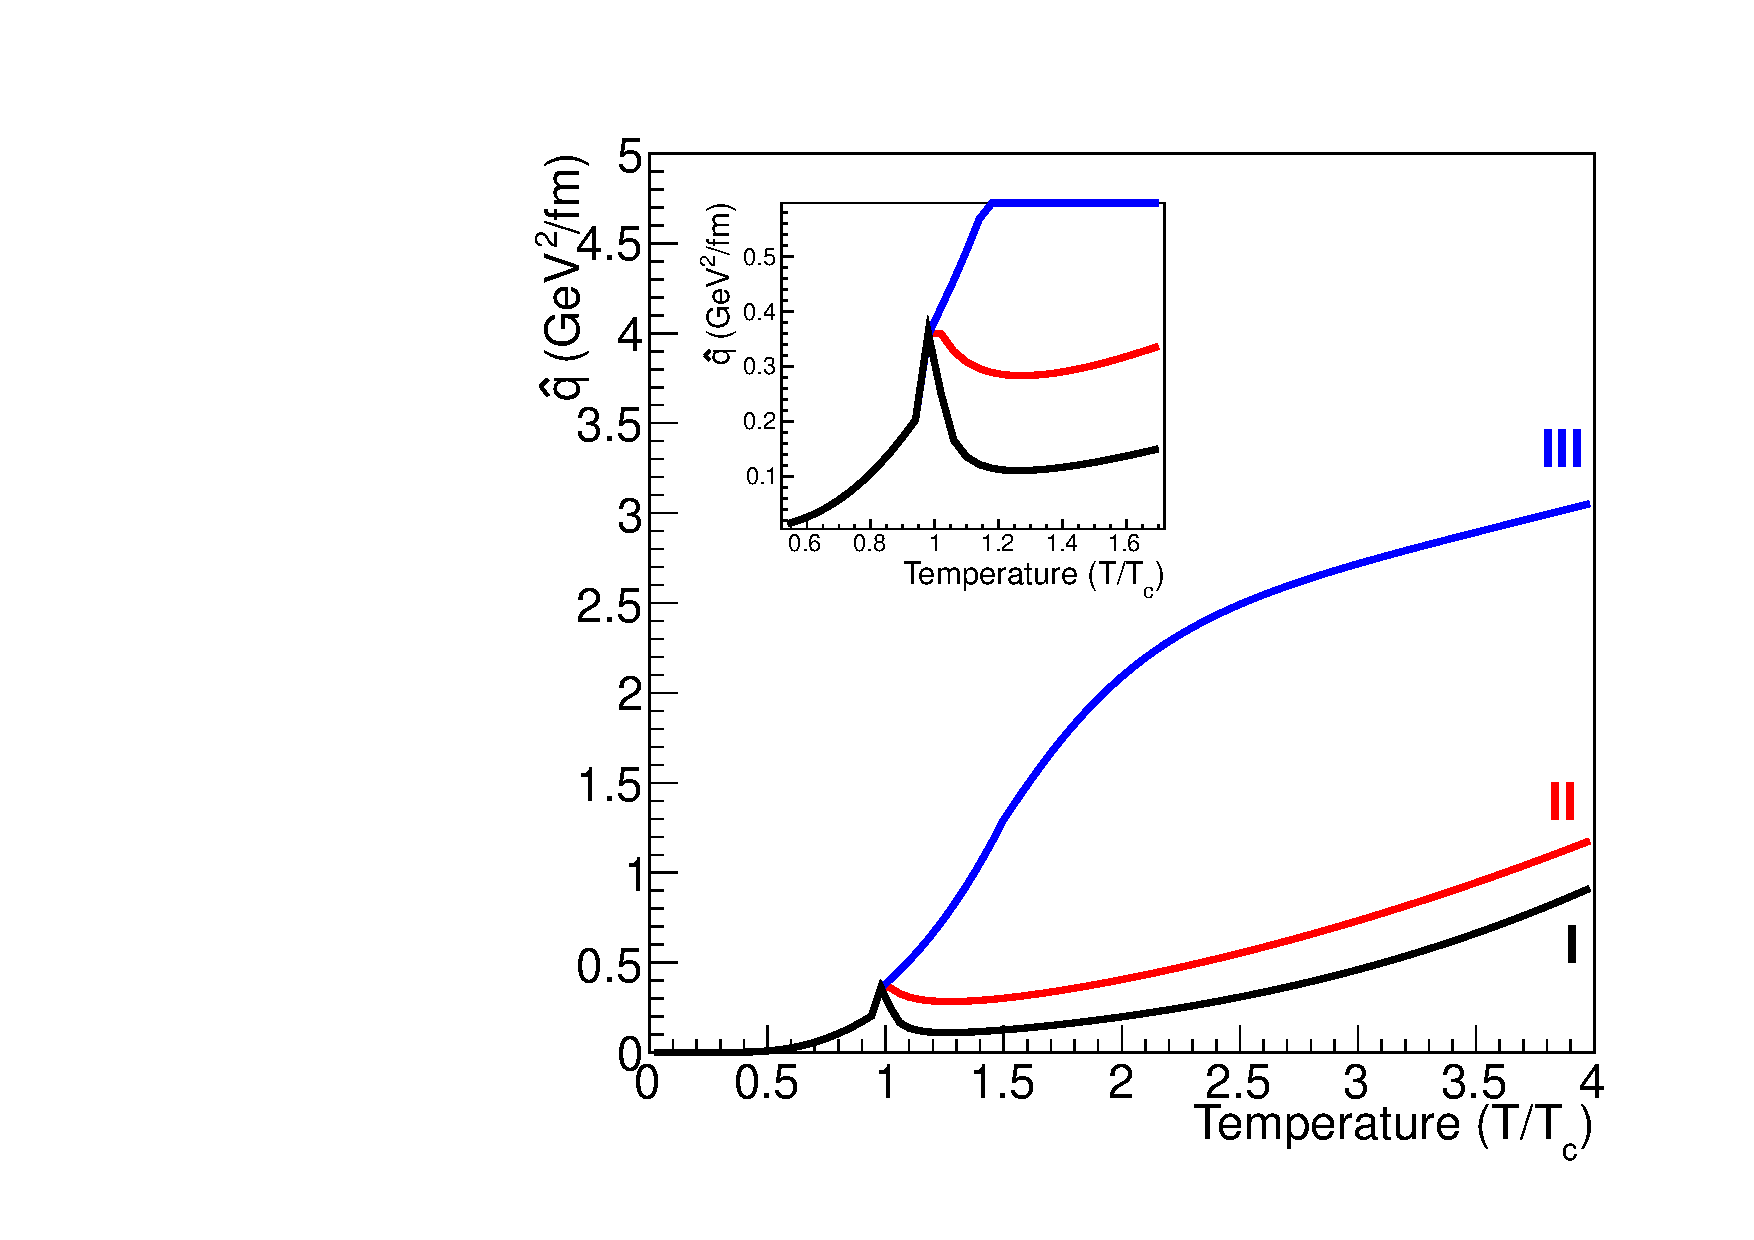
\includegraphics[trim = 2 2 2 2, clip, width=\twowidth]{figs/figure_physicscase_qhatscenarios_modscen1}
%    \hfill
%    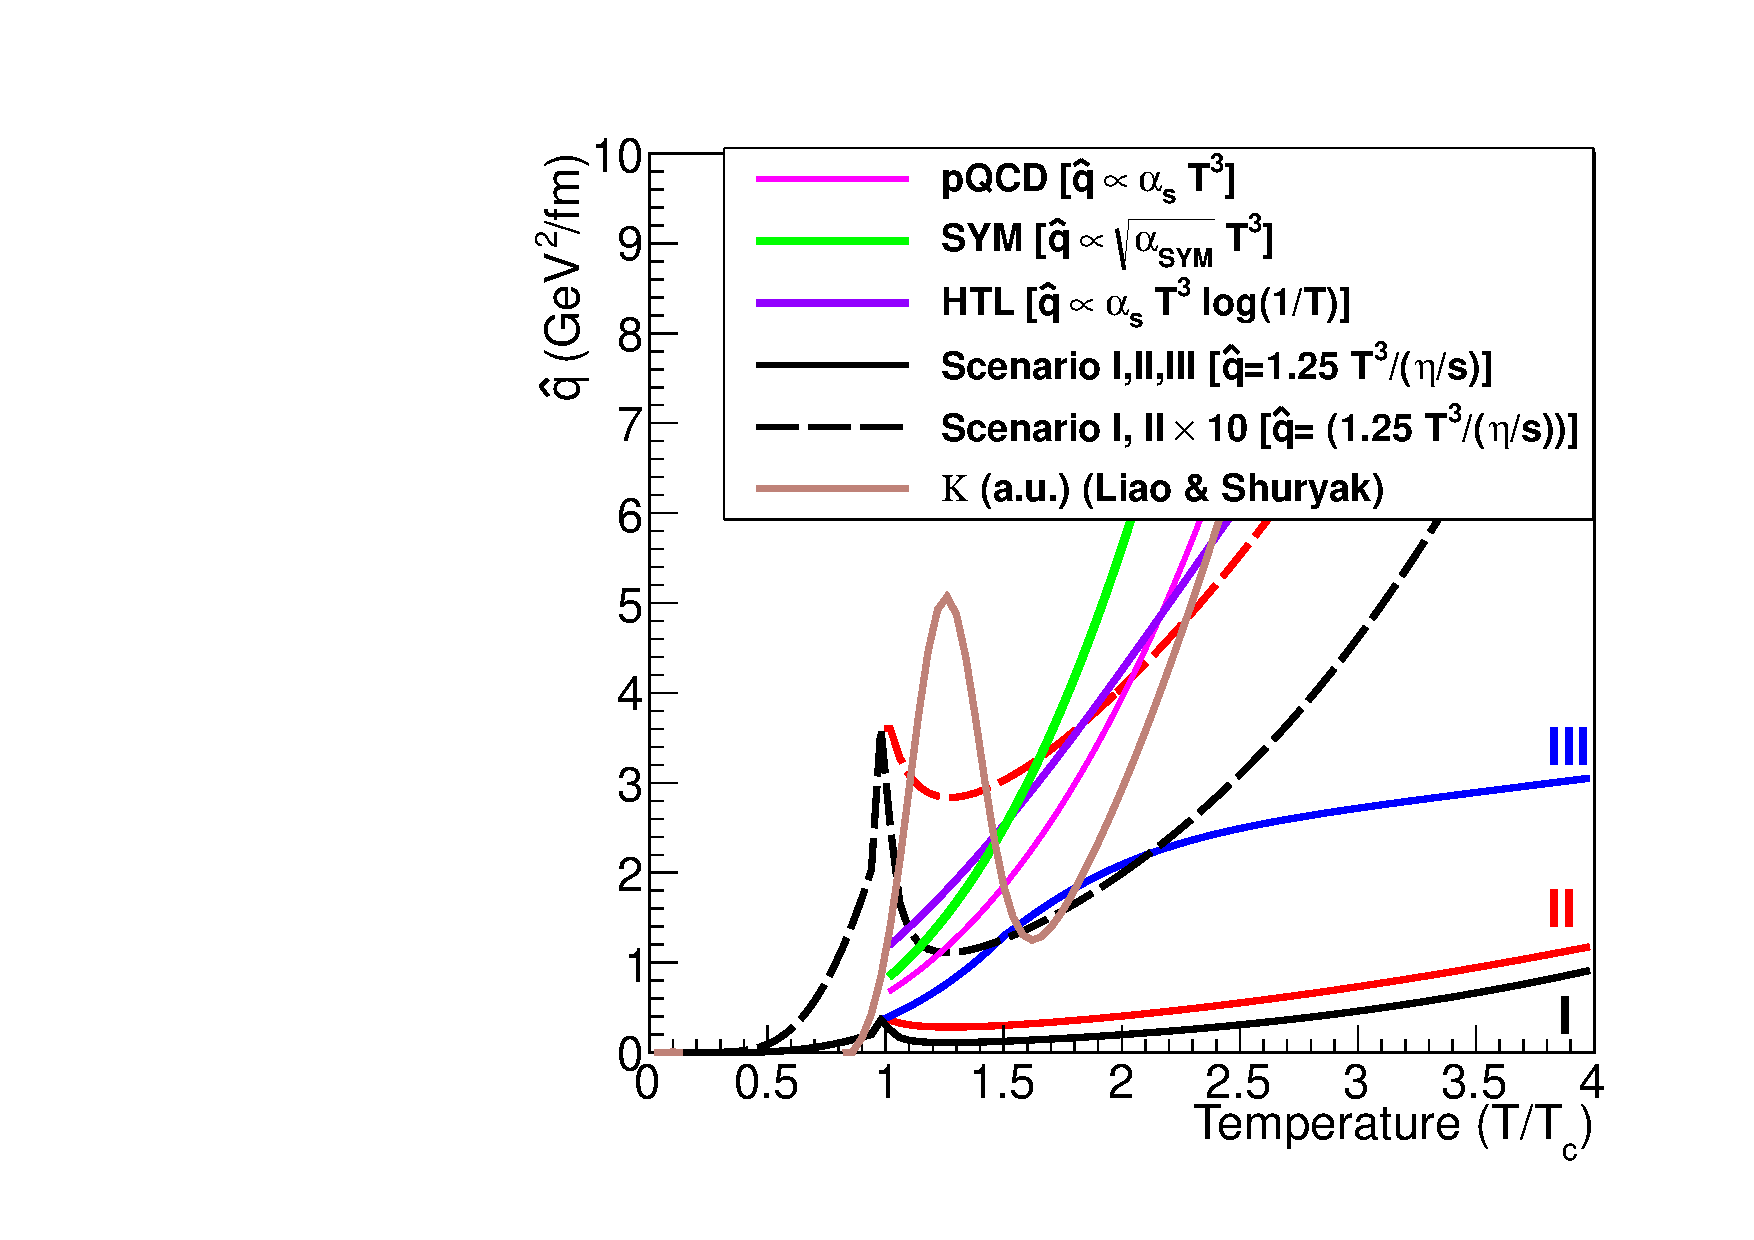
\includegraphics[trim = 2 2 2 2, clip, width=\twowidth]{figs/figure_physicscase_qhatscenarios_all_modscen1}
%    \caption[$\hat{q}$ vs $T/T_{c}$ in weak and strong coupling
%    scenarios]{(left) $\hat{q}$ as a function of $T/T_{c}$ in the
%      three scenarios as related with the weak-coupling
%      calculation. (right) Different calculations for the scaling of
%      $\hat{q}$ under weak and strong coupling assumptions.}
%    \label{fig:qhatmap}
% \end{center}
%\end{figure}

%Figure~\ref{fig:qhatmap} (right panel) shows that for the equivalence
%relation of Eqn.~\ref{eq:qhat2etas}, all three scenarios have a result
%that differs significantly from the simple perturbative expectation of
%$\alpha_{s} T^{3}$~\cite{Armesto:2011ht}.  Also shown in
%Figure~\ref{fig:qhatmap} are the predicted temperature dependence of
%$\hat{q}$ in the strongly coupled AdS/CFT (supersymmetric Yang-Mills)
%case~\cite{Liu:2006ug} and the Hard Thermal Loop (HTL)
%case~\cite{arnold:2000dr}.

%There is enormous room for experimental measurements to provide key insights
%and constraints on the evolution of the jet quenching power.  

Since the expected scaling of $\hat{q}$ with temperature is such a
strong function of temperature, jet quenching measurements should be
dominated by the earliest times and highest temperatures.  In order
to have sensitivity to temperatures around 1--2 $T_c$, measurements
at RHIC are needed in contrast to the LHC where larger initial
temperatures are produced.  In addition, the ability of RHIC to
provide high luminosity heavy-ion collisions at a variety of center
of mass energies can be exploited to probe the detailed temperature
dependence of quenching right in the vicinity of $T_c$.

Theoretical developments constrained simultaneously by data from RHIC and the LHC 
have been important in discriminating against some models with very
large $\hat{q}$  -- see Figure~\ref{fig:cmsqhat} from Ref.~\cite{CMS:2012aa} and theory
references therein.  Models such as PQM and ASW with very large values of $\hat{q}$ have been ruled out
by the combined constraint.  Shown in the left panel of Figure~\ref{fig:qhatconstraint} is a recent compilation of four
theoretical calculations with a directly comparable extraction of $\hat{q}$.  Developments on the 
theory and experimental fronts have significantly narrowed the 
range of $\hat{q}$~\cite{JETCollaboration:QhatConstraint}.
This theoretical progress lends strength to the case that the tools will be
available on the same time scale as sPHENIX data to have precision determinations
of $\hat{q}$ and then ask deeper additional questions about the \qgp and its underlying properties.

\begin{figure}[ht]
  \centering
  \raisebox{0.2cm}{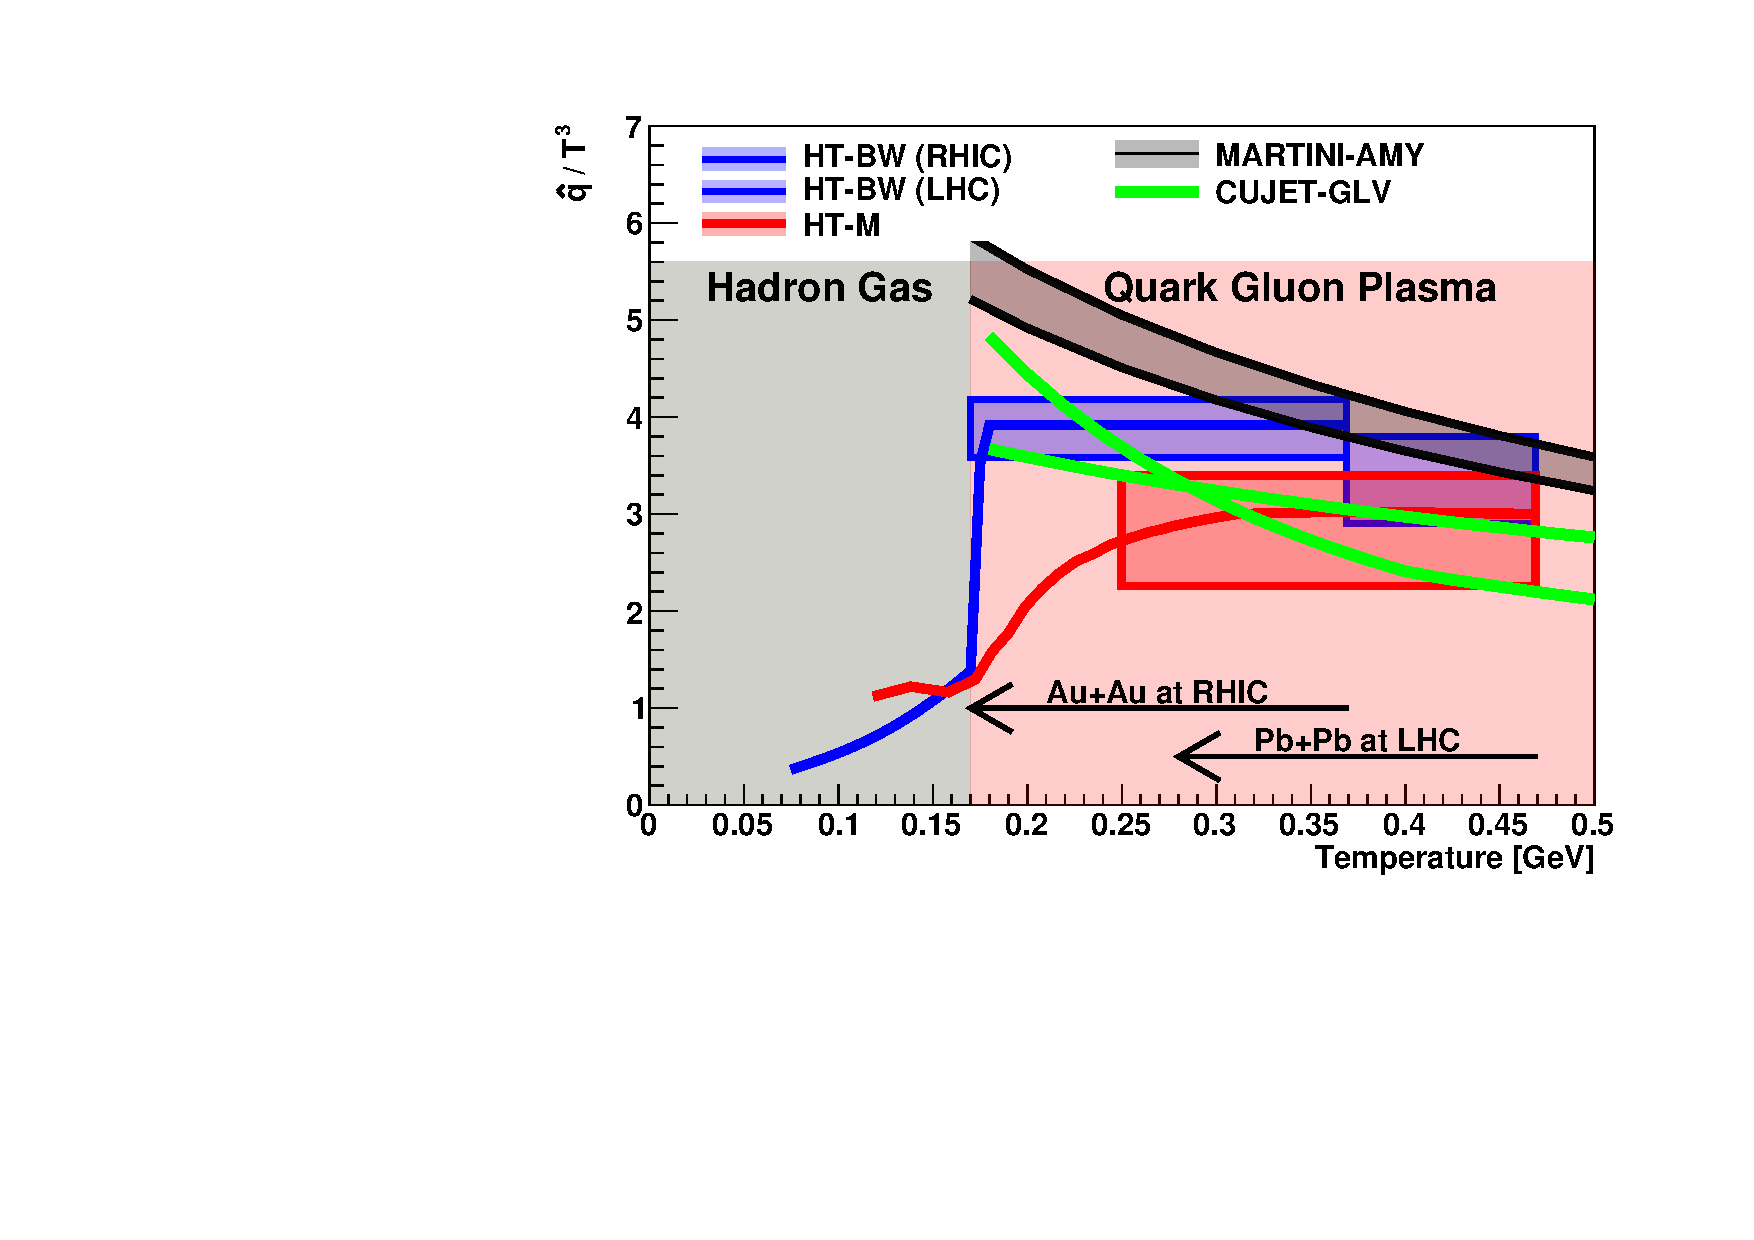
\includegraphics[width=0.49\linewidth]{figs/figure_qhatconstraint}}
  \hfill
  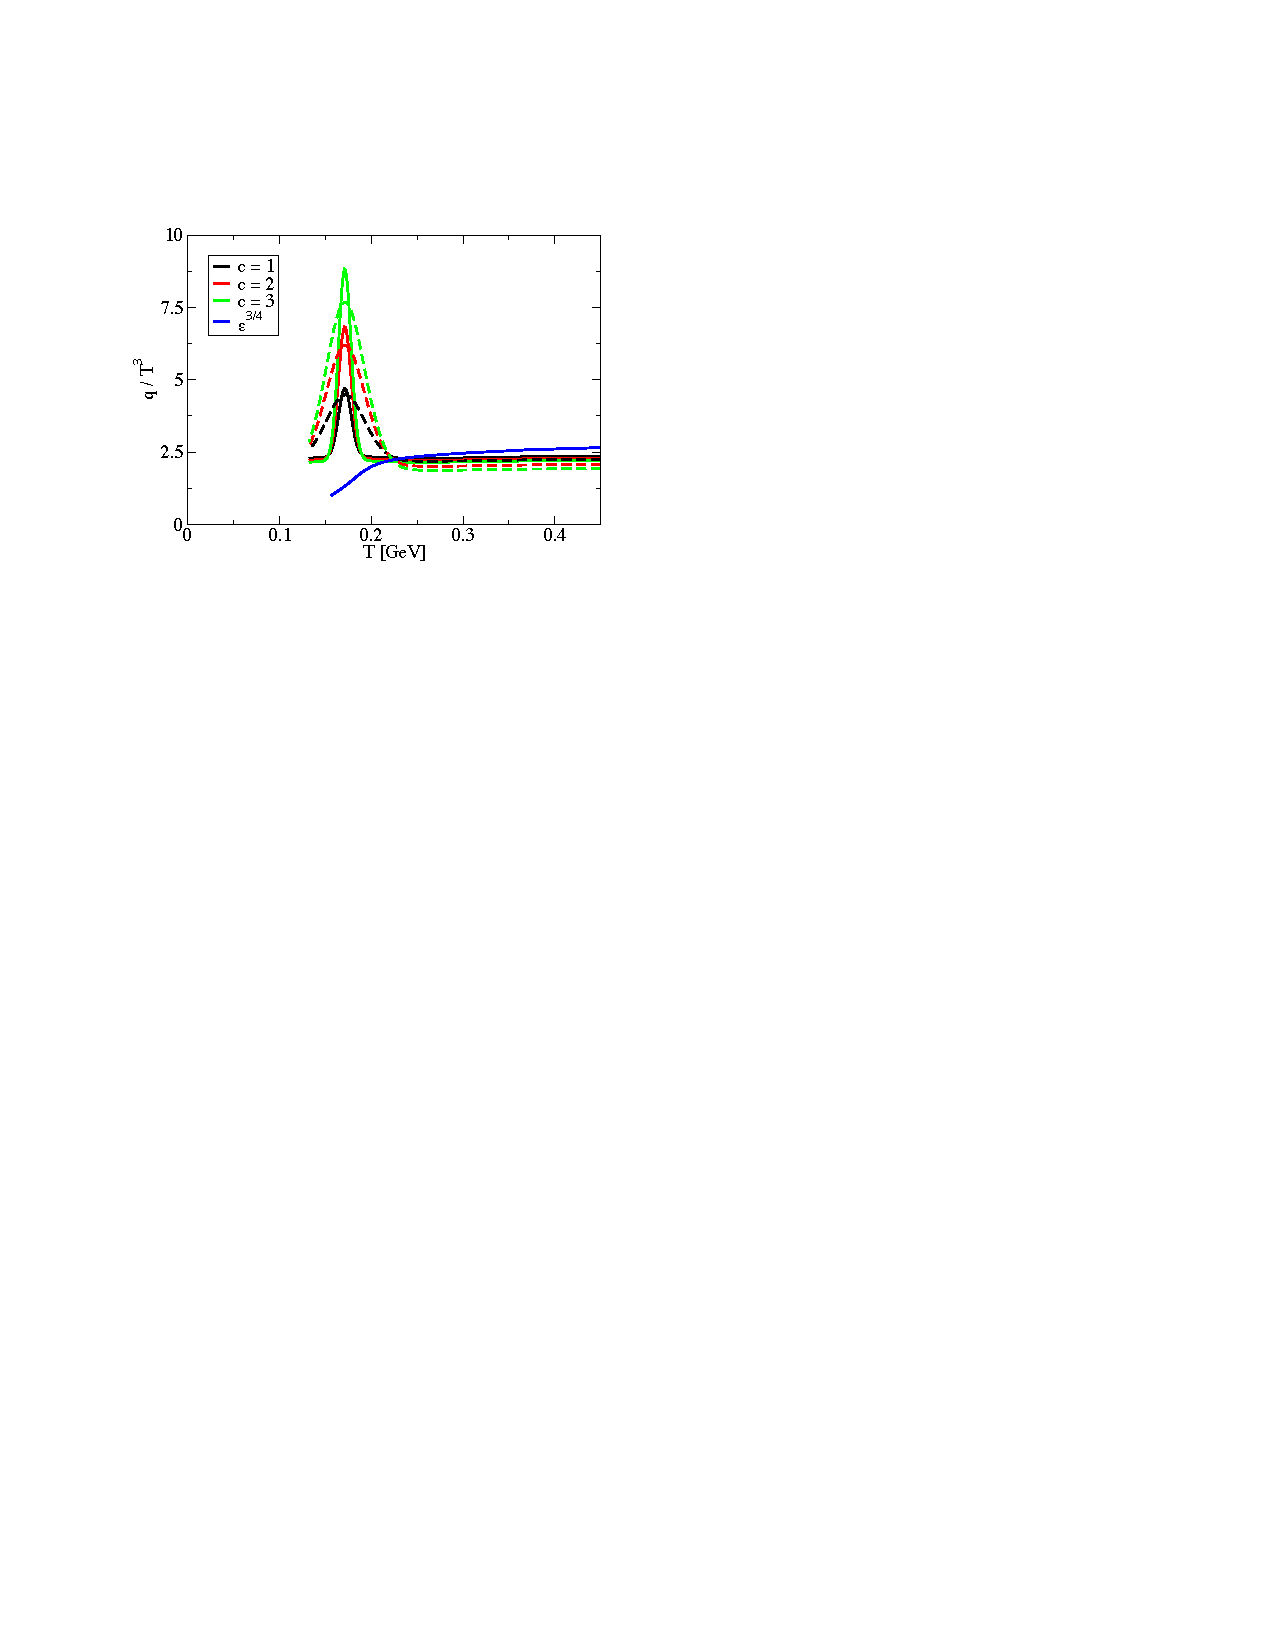
\includegraphics[width=0.49\linewidth]{figs/ntce_renk}
  \caption[Calculations of $\hat{q}/T^{3}$ vs temperature, constrained
  by RHIC and LHC \raa data --- including near $T_C$ enhancement
  scenarios of $\hat{q}/T^{3}$]{(left) Calculations from four jet
    quenching frameworks constrained by RHIC and LHC \raa data
    with results for $\hat{q}/T^{3}$ as a function of temperature.
    Details of the calculation are given in
    Ref.~\cite{JETCollaboration:QhatConstraint}. (right) Near $T_C$
    enhancement scenarios of $\hat{q}/T^{3}$ considered in
    Ref.~~\cite{Renk:2014nwa}.}
  \label{fig:qhatconstraint}
\end{figure}

It is notable that a number of calculations favor an increased coupling strength near the transition temperature.  Shown in the right panel of Figure~\ref{fig:qhatconstraint} are a set of scenarios
considered by Renk in Ref.~\cite{Renk:2014nwa}.   This paper states that ``Comparing weak coupling scenarios with data, 
NTC [near $T_{C}$ enhancement] is favored.   An answer to this question will require a systematic picture 
across several different high \pt observables.''   

In Ref.~\cite{Liao:2008dk}, Liao and Shuryak use 
RHIC measurements of single hadron suppression and azimuthal
anisotropy to infer that ``the jet quenching is a few times stronger
near $T_c$ relative to the quark-gluon plasma at $T > T_c$.''  This
enhancement of $\hat{q}$ is shown in Figure~\ref{fig:qhatmap} (right panel)
and is the result of color magnetic monopole excitations in the plasma
near $T_{c}$.   

Most recently this strong coupling picture with color magnetic monopole excitations has been
implemented within CUJET 3.0 for a broader comparison with experimental observables and
previous theory calculations~\cite{Xu:2014tda}.   Shown in Figure~\ref{fig:cujet_monopole} are
results from their constrained RHIC and LHC data fit for the temperature dependence of the scaled
quenching power $\hat{q}/T^{3}$.

\begin{figure}[ht]
  \centering
  \raisebox{0.2cm}{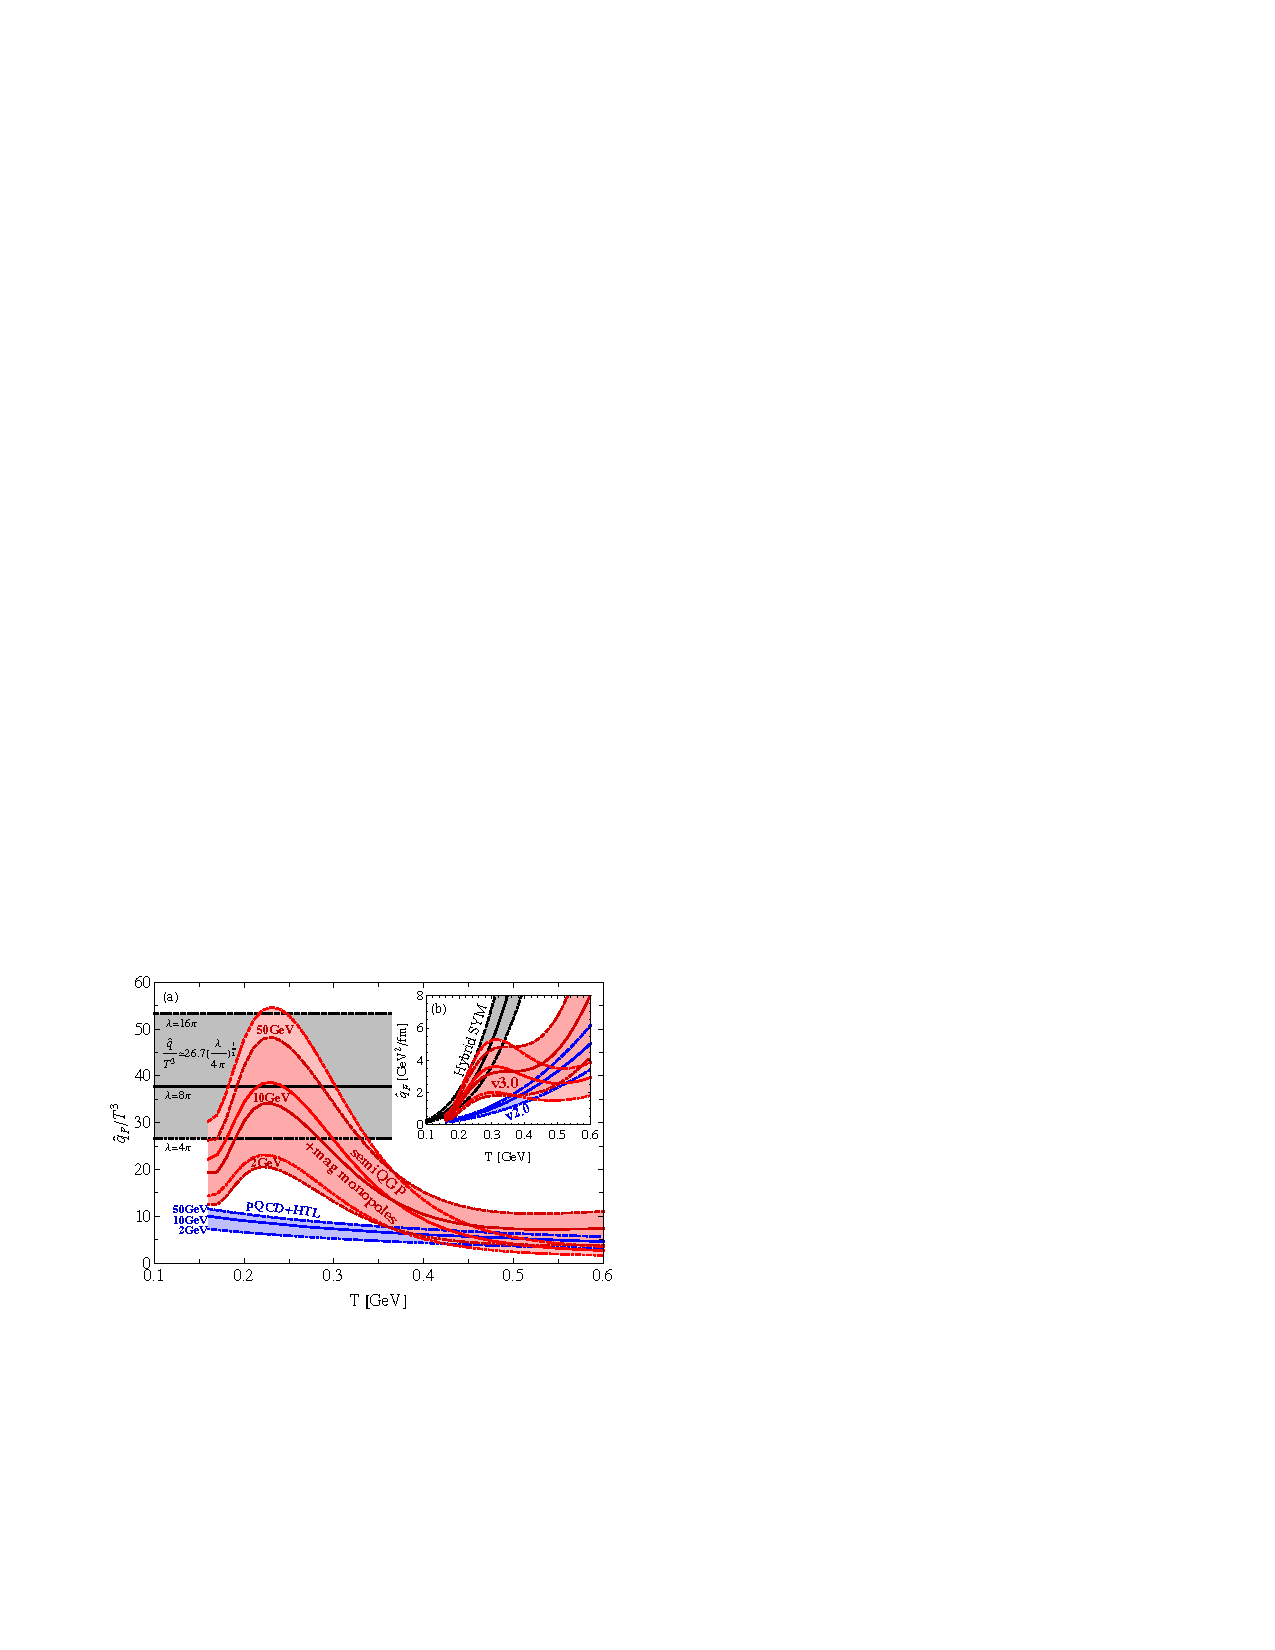
\includegraphics[width=0.68\linewidth]{figs/figure_cujet_qhat}}
  \caption[Magnetic Monopole/CUJET 3.0 result for $\hat{q}/T^{3}$ vs temperature, constrained
  by RHIC and LHC \raa data]{Results from calculations within CUJET 3.0 with magnetic monopole
excitations that result in enhanced coupling near $T_{c}$.   Plotted are the constraints on $\hat{q}/T^{3}$ 
as a function of temperature as shown in Ref.~~\cite{Xu:2014tda}.}
  \label{fig:cujet_monopole}
\end{figure}

Within the jet quenching model WHDG~\cite{Horowitz:2011gd}, the authors 
constrain $\hat{q}$ by the PHENIX $\pi^{0}$ nuclear modification factor.  
They find the prediction scaled by the expected increase in the color charge 
density created in higher energy LHC collisions when compared to the ALICE
results~\cite{Aamodt:2010jd} over-predicts the suppression.
This over-prediction based on the assumption of an unchanging probe-medium
coupling strength led to title of Ref.~\cite{Horowitz:2011gd}: ``The
surprisingly transparent sQGP at the LHC.''  They state that ``one
possibility is the sQGP produced at the LHC is in fact more
transparent than predicted.''  Similar conclusions have been reached
by other authors~\cite{Chen:2011vt,Zakharov:2011ws,Buzzatti:2011vt}.
Recently work has been done to incorporate the running of the QCD coupling
constant~\cite{Buzzatti:2012dy}.  

It is important to note that most all calculations predict a stronger
coupling near the transition, even if just from the running of the
coupling constant $\alpha_{s}$, and the goal is to experimentally
determine the degree of the effect.  Lower energy data at RHIC also
provides important constraints -- see for example
Refs.~\cite{Adare:2012uk,Schmah:2013vea}.  The full set of
experimental observables need to be considered spanning the largest
range of collision energy, system size, and engineering path length.

One observable that has been particularly challenging for energy loss
models to reproduce is the azimuthal anisotropy of $\pi^0$ production
with respect to the reaction plane.  A weak dependence on the path
length in the medium is expected from radiative energy loss.  This
translates into a small $v_2$ for high $p_T$ particles (i.e., only a
modest difference in parton energy loss when going through a short
versus long path through the QGP).  

%Results of $\pi^0$ $v_2$ are shown
%in Figure~\ref{fig:phenixpi0v2}~\cite{Adare:2010sp}.  Weakly coupled
%radiative energy loss models are compared to the \raa (bottom
%panels) and $v_2$ (top panels) data.  These models reproduce the
%\raa, but they fall far short of the $v_2$ data in both $p_T$
%ranges measured (6--9~GeV/c and $>9$~GeV/c).  

The large path length
dependence is naturally described by strongly coupled energy loss
models~\cite{Marquet:2009eq,Adare:2010sp}.  Note that one can match
the $v_2$ by using a stronger coupling, larger $\hat{q}$, but at the
expense of over-predicting the average level of suppression.  New
strong coupling
models~\cite{Casalderrey-Solana:2014wca,Casalderrey-Solana:2014bpa}
also need to confront the full data set available at RHIC.

%\begin{figure}[!hbt]
% \begin{center}
%    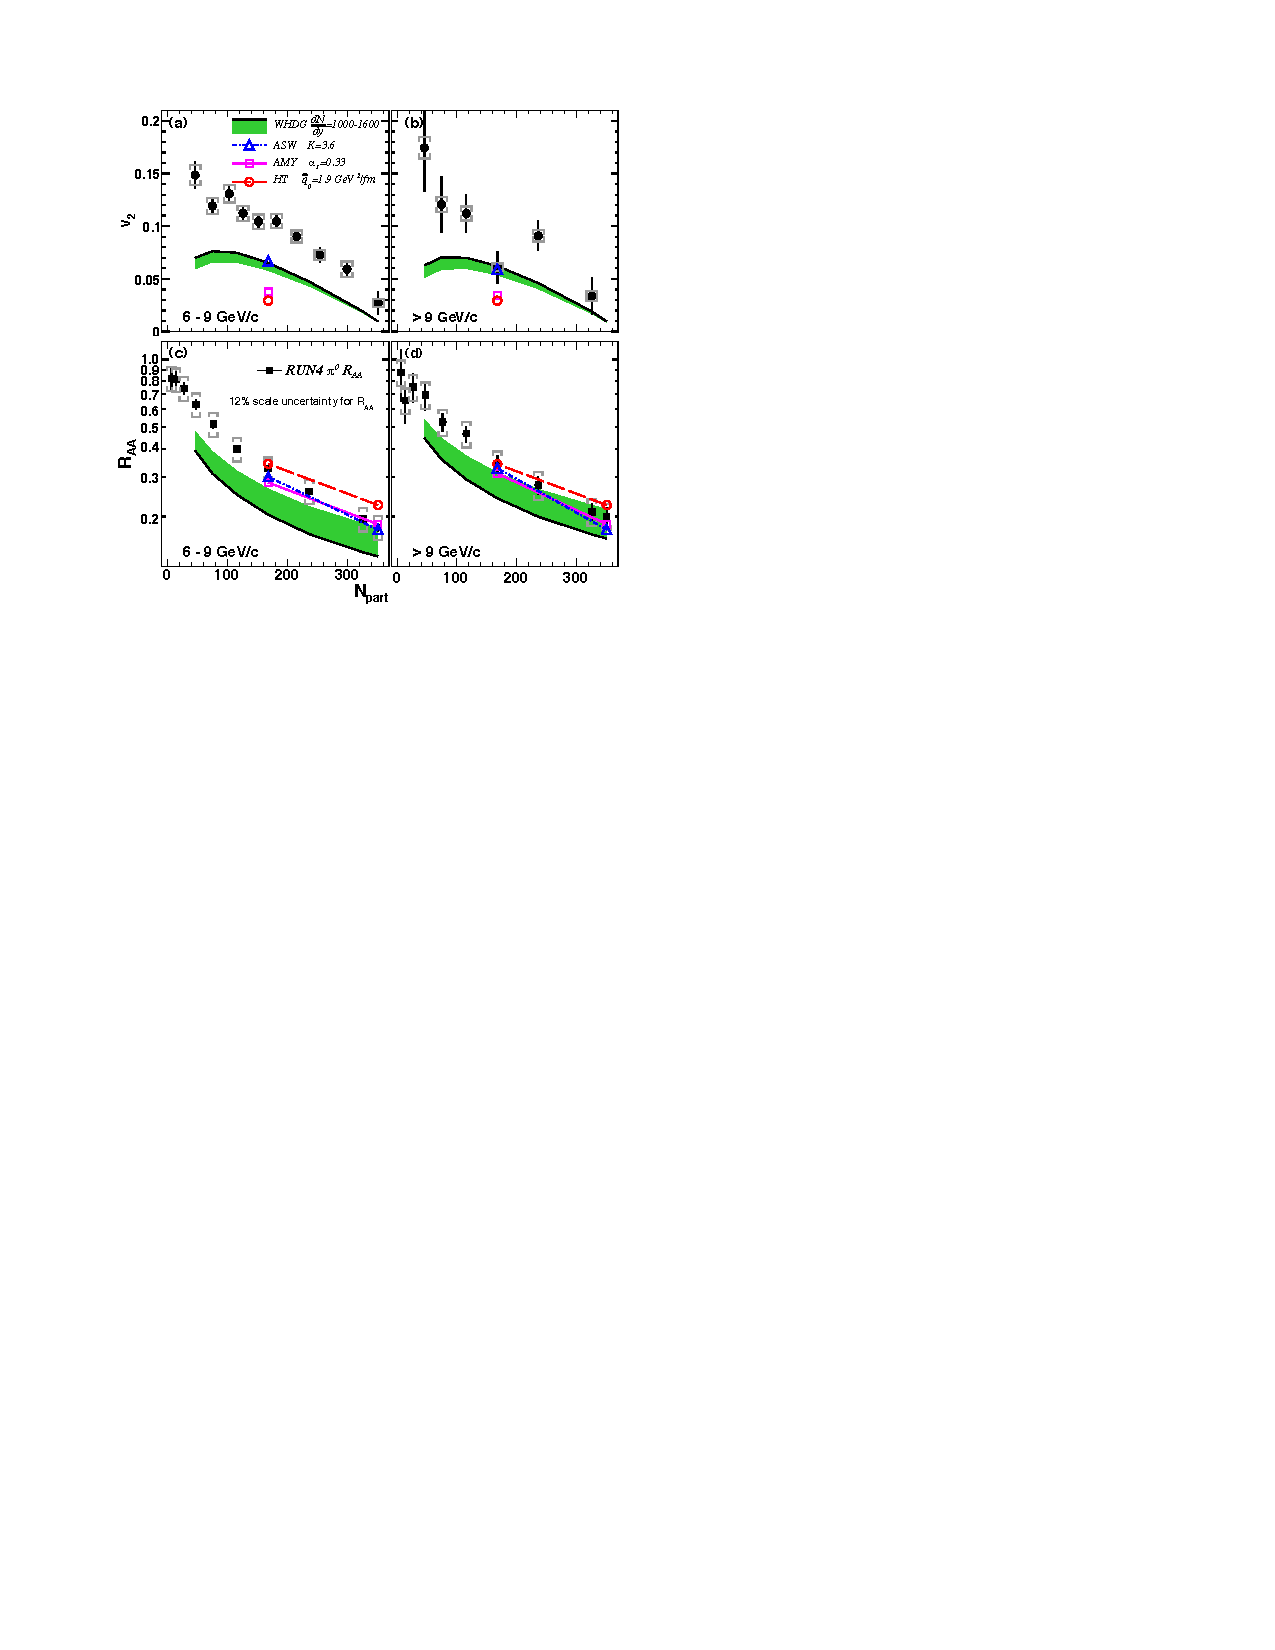
\includegraphics[trim = 2 2 2 2, clip, width=0.6\linewidth]{figs/figure_physicscase_phenix_hadronv2}
%    \caption[Experimental $\pi^0$ $v_2$ and \raa along with
%    calculations from four weakly coupled energy loss
%    models]{\label{fig:phenixpi0v2} $\pi^0$ $v_2$
%      (top panels) and \raa (bottom panels) for $6<p_T<9$~GeV/c
%      (left panels) and $p_T>9$~GeV/c (right panels).  Calculations
%      from four weakly coupled energy loss models are shown as
%      well~\cite{Bass:2008rv,Wicks:2005gt}.  From
%      Ref.~\protect\cite{Adare:2010sp}{}.}
%  \end{center}
%\end{figure}

The measurement of jet quenching observables as a detailed function of
orientation with respect to the reaction plane is directly sensitive
to the coupling strength and the path length dependence of the
modification to the parton shower.  In addition, medium response may
be optimally measured in mid-central collisions with a lower
underlying event and where the medium excitations are not damped out
over a longer time evolution.  Shown in
Figure~\ref{fig:sPHENIX_AuAu_ReactionPlane_figure} are projected
uncertainties from sPHENIX --- detailed in the chapter on physics
performance --- for the direct photon and reconstructed jet observables
in three orientation selections.  One expects no orientation
dependence for the direct photons and the question is whether the
unexpectedly large dependence for charged hadrons persists in
reconstructed jets up to the highest \pt.  Note that the same
measurements can be made for beauty tagged jets, charged hadrons up to
50 GeV/c, and a full suite of correlation measurements including
jet-jet, hadron-jet, $\gamma$-jet.

\begin{figure}[t]
 \begin{center} % dvp
    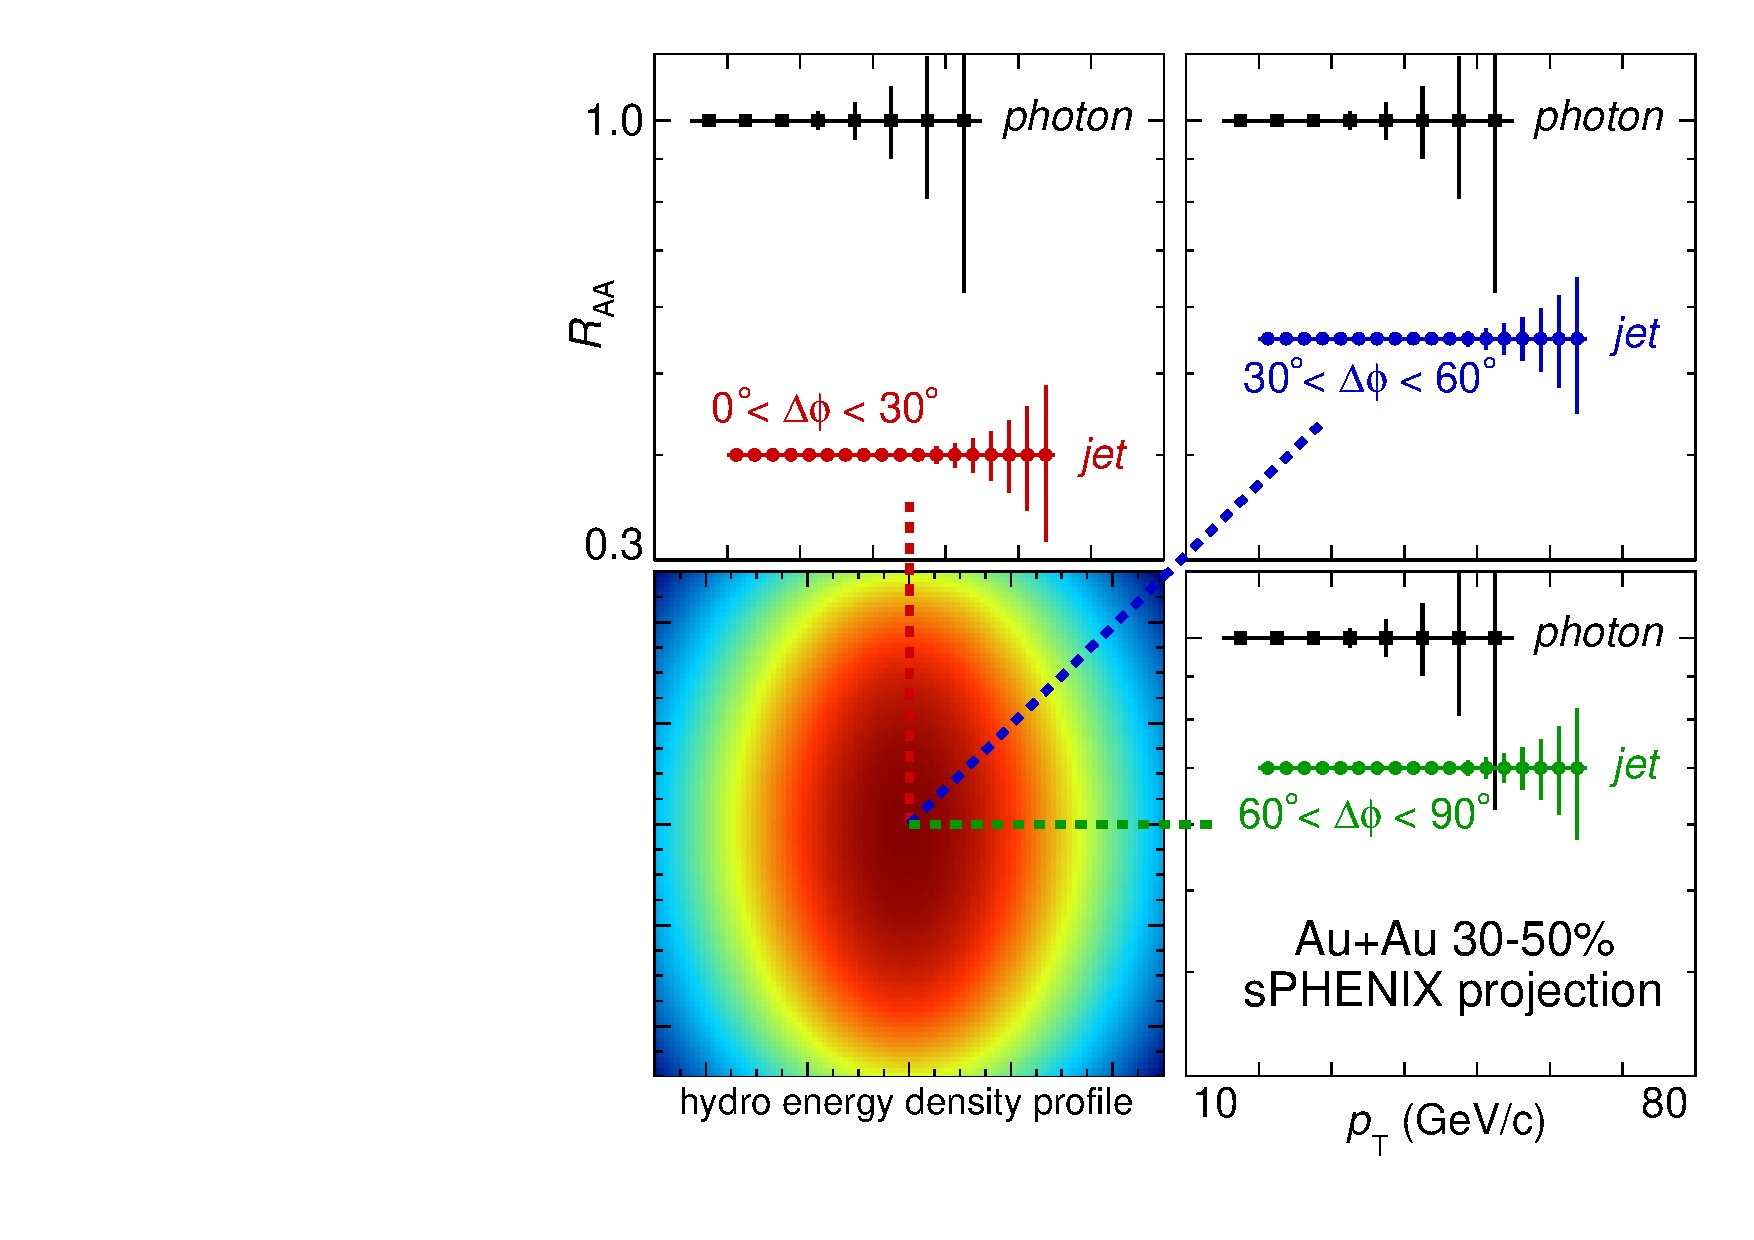
\includegraphics[width=0.8\linewidth]{figs/sPHENIX_MIE_AuAu_ReactionPlane_figure}
    \caption[Statistical reach of azimuthally-sensitive hard probes in
    sPHENIX]{Demonstration of the statistical reach for
      azimuthally-sensitive hard probes measurements in sPHENIX. Each
      panel shows the projected statistical uncertainty for the
      $R_\mathrm{AA}$ of inclusive jets and photons, with each a panel
      a different $\Delta\phi$ range with respect to the reaction
      plane in $30$--$50$\% Au+Au events. sPHENIX would additionally
      have tremendous statistical reach in the analogous charged
      hadron
      $R_\mathrm{AA}$. \label{fig:sPHENIX_AuAu_ReactionPlane_figure} }
    \end{center}
\end{figure}

All measurements in heavy ion collisions are the result of emitted
particles integrated over the entire time evolution of the reaction,
covering a range of temperatures.  Similar to the hydrodynamic model constraints, the
theory modeling for jet probes requires a consistent temperature and scale dependent
model of the \qgp and is only well constrained by precision data through
different temperature evolutions, as measured at RHIC and the LHC.

%\clearpage

\section{What are the inner workings of the QGP?}
\label{Section:InnerWorkings}

A second axis along which one can investigate the underlying
structure of the \qgp concerns the question of what length scale of
the medium is being probed by jet quenching processes.  In
electron scattering, the scale is set by the virtuality of the
exchanged photon, $Q^{2}$. By varying this virtuality one can
obtain information over an enormous range of scales: from
pictures of viruses at length scales of $10^{-5}$ meters, to the
partonic make-up of the proton in deep inelastic electron scattering
at length scales of less than $10^{-18}$ meters. 

For the case of hard scattered partons in the quark-gluon plasma, the length scale probed
is initially set by the virtuality of the hard scattering process.  Thus, at the
highest LHC jet energies, the parton initially probes a very short length scale.  
Then as the evolution proceeds, the length scale is set by
the virtuality of the gluon exchanged with the
color charges in the medium, as shown in the left panel of
Figure~\ref{fig:probescale}.  However, if the exchanges are coherent, 
%the length scale is simply set by the individual exchange
%gluon virtuality or instead by 
the total coherent energy loss through
the medium may set the length scale.

\begin{figure}[!hbt]
 \begin{center}
   \raisebox{0.05in}{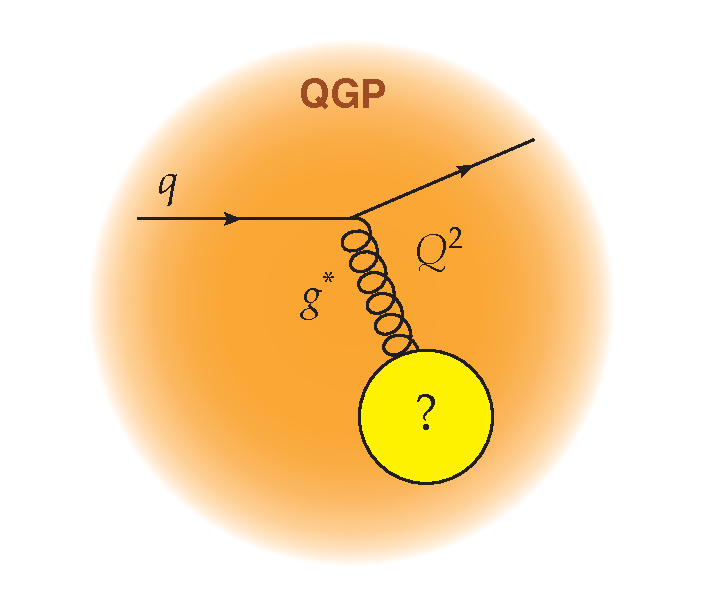
\includegraphics[trim = 2 2 2 2, clip,width=0.57\linewidth]{figs/figure_physicscase_probescale1}}
    \hfill
    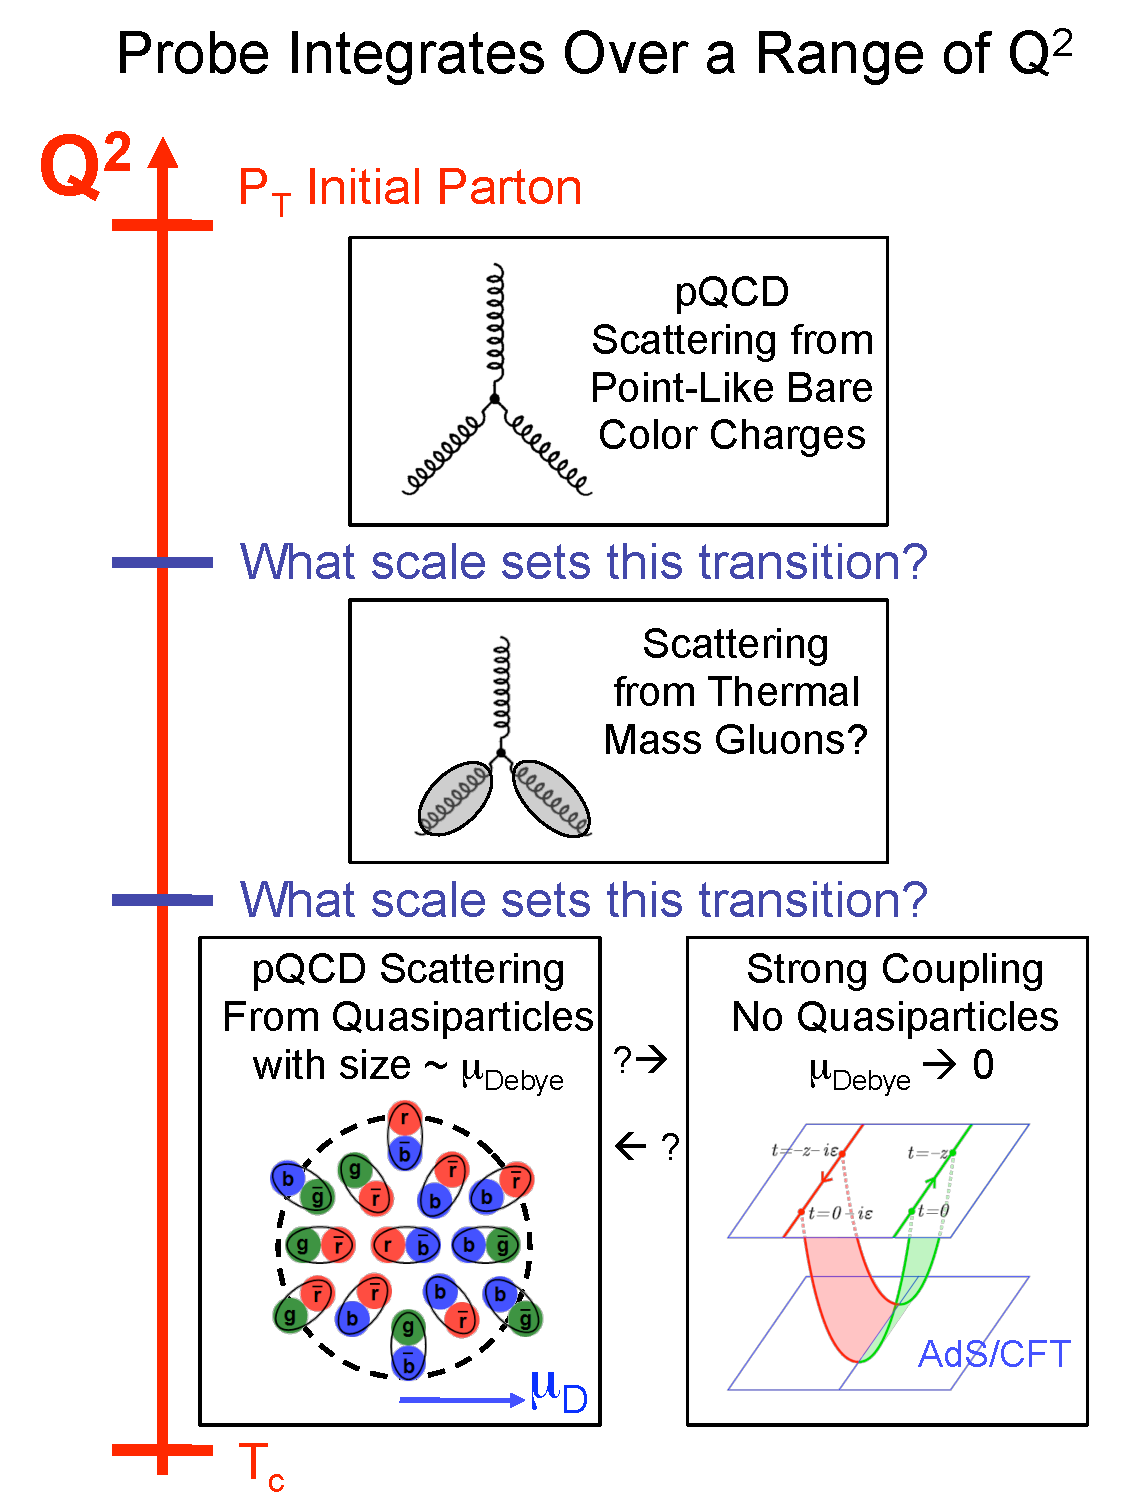
\includegraphics[trim = 2 2 2 50, clip,width=0.4\linewidth]{figs/figure_physicscase_probescale2}
    \caption[Interaction scale for the interaction of partons with the
    \qgp and possibilities for the recoil objects]{(left) Diagram of a
      quark exchanging a virtual gluon with an unknown object in the
      QGP.  This highlights the uncertainty for what sets the scale of
      the interaction and what objects or quasiparticles are
      recoiling.  (right) Diagram as a function of the $Q^{2}$ for the
      net interaction of the parton with the medium and the range of
      possibilities for the recoil objects.\label{fig:probescale}}
 \end{center}
\end{figure}

Figure~\ref{fig:probescale} (right panel) shows that if the length
scale probed is very small then one expects scattering directly from
point-like bare color charges, most likely without any influence from
quasiparticles or deconfinement.  As one probes longer length
scales, the scattering may be from thermal mass gluons and eventually
from possible quasiparticles with size of order the Debye screening
length.  In Ref.~\cite{krishna}, Rajagopal states that ``at some length scale, a
quasiparticulate picture of the QGP must be valid, even though on its
natural length scale it is a strongly coupled fluid.  It will be a
challenge to see and understand how the liquid QGP emerges from
short-distance quark and gluon quasiparticles.''

The extension of jet measurements over a wide range of energies and
with different medium temperatures again gives one the largest span
along this axis.  What the parton is scattering from in the medium is
tied directly to the balance between radiative energy loss and
inelastic collisional energy loss in the medium (encoded in $\hat{q}$ and $\hat{e}$). 
In the limit that the scattering centers in the medium are infinitely massive, one only
has radiative energy loss---as was assumed for nearly 10 years to be
the dominant parton energy loss effect.  In the model of Liao and
Shuryak~\cite{Liao:2008dk}, the strong coupling near the quark-gluon
plasma transition is due to the excitation of color magnetic
monopoles, and this should have a significant influence on the
collisional energy loss and equilibration of soft partons into the
medium.

In a model by Coleman-Smith~\cite{ColemanSmith:2011rw,ColemanSmith:2011wd}
consisting of parton showers propagating in a medium of deconfined
quarks and gluons, one can directly vary the mass of the effective scattering centers and extract
the resulting values for $\hat{e}$ and $\hat{q}$.
Figure~\ref{fig:ehat_qhat} shows $T\hat{e}/\hat{q}$ as a function of
the mass of the effective scattering centers in the medium in this
model.  In the limit of infinitely massive scattering centers, the
interactions are elastic and no energy is transferred to the medium.
\begin{figure}[ht]
  \centering
  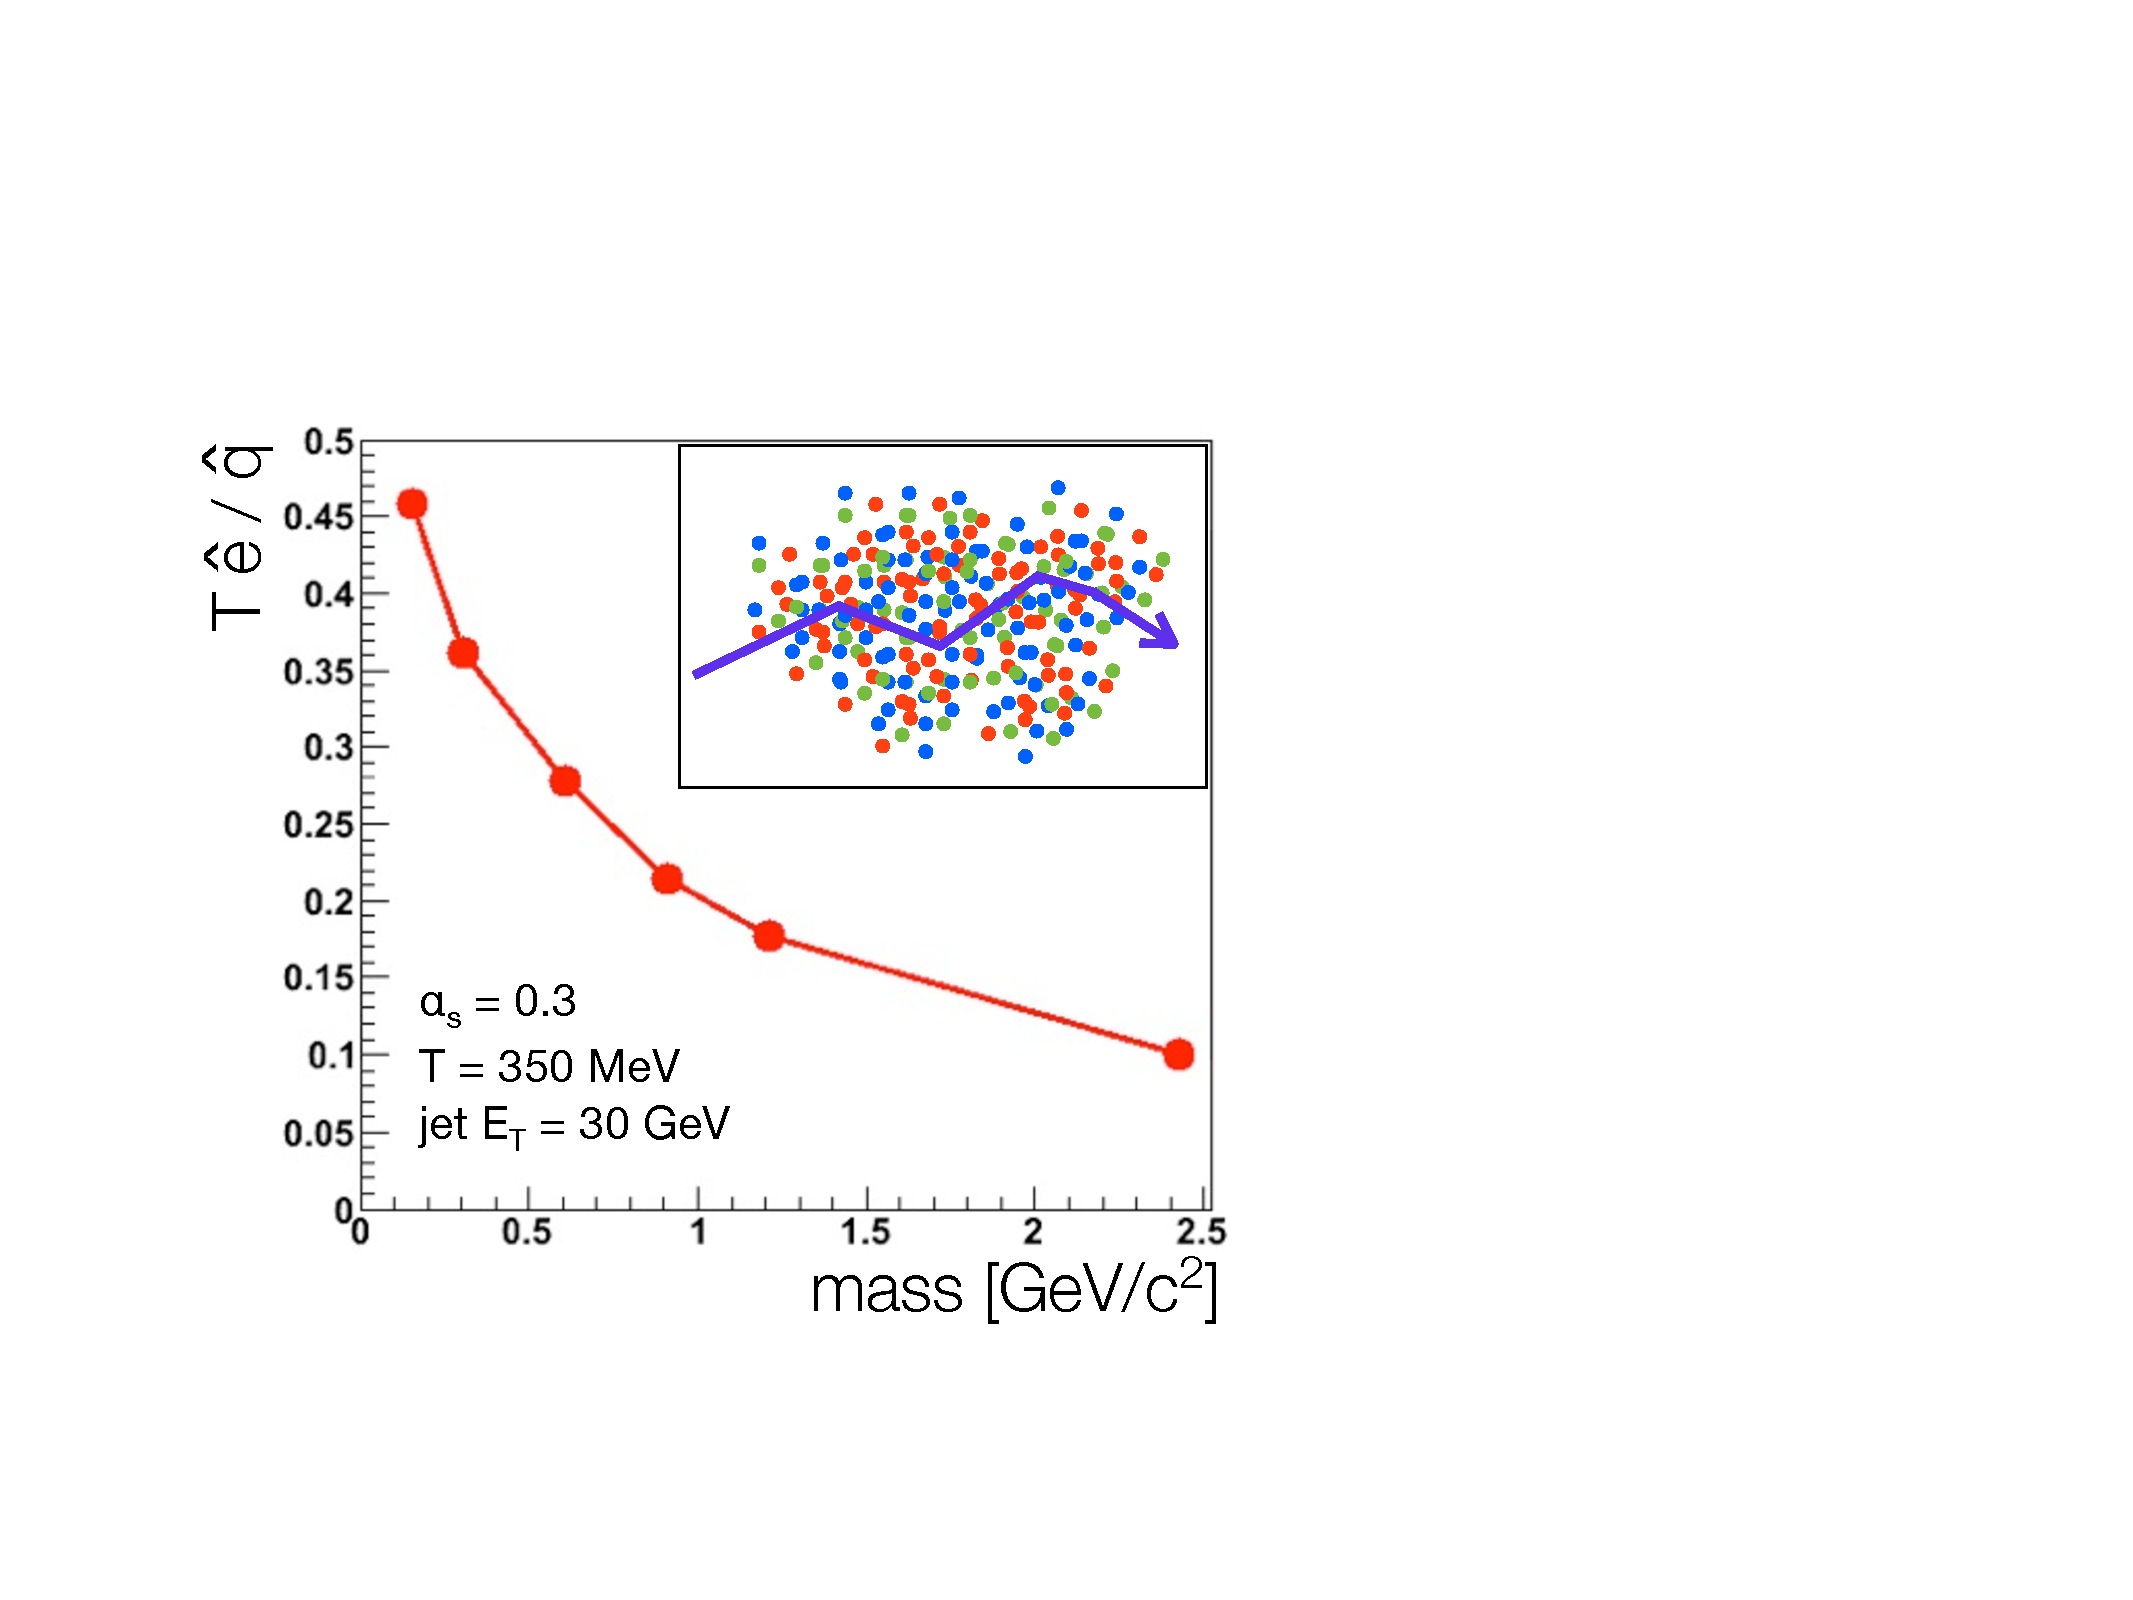
\includegraphics[width=0.6\linewidth]{figs/figure_coleman_mass}
  \caption[$T\hat{e}/\hat{q}$ as a function of the mass of the
  effective scattering centers in the medium]{$T\hat{e}/\hat{q}$ as a
    function of the mass of the effective scattering centers in the
    medium.  As the mass increases, the parton is less able to
    transfer energy to the medium and the ratio drops.}
  \label{fig:ehat_qhat}
\end{figure}

%Many observables are sensitive to the balance of $\hat{e}$ and $\hat{q}$, %and thus sensitive to what is being
%scattered from in the medium.   For example, in the same calculation by Coleman-Smith~\cite{ColemanSmith:2012vr}, 
%the transverse radial jet energy profile is significantly modified by the balance of collisional and radiative energy loss.   Shown 
%in the left panels Figure~\ref{fig:csjetprofile} are the vacuum and medium modified fractional energy distribution as a function
%of distance $R$ from the jet axis.   The upper left panel is including both elastic and inelastic processes and the 
%lower left panel with only elastic processes.    In the right panel we show the ratio of the profiles and for three different
%effective medium coupling parameters. The sub-leading jet profiles are
%dramatically modified compared to the vacuum and leading jet profiles. The elastic and radiative profiles clearly
%separate, the radiative sub-leading jets become broader and softer than the elastic only. Both sets of sub-leading jets
%become much broader and softer compared to the leading jets.

%\begin{figure}[!hbt]
% \begin{center}
%   \begin{minipage}[c]{0.27\textwidth}
%     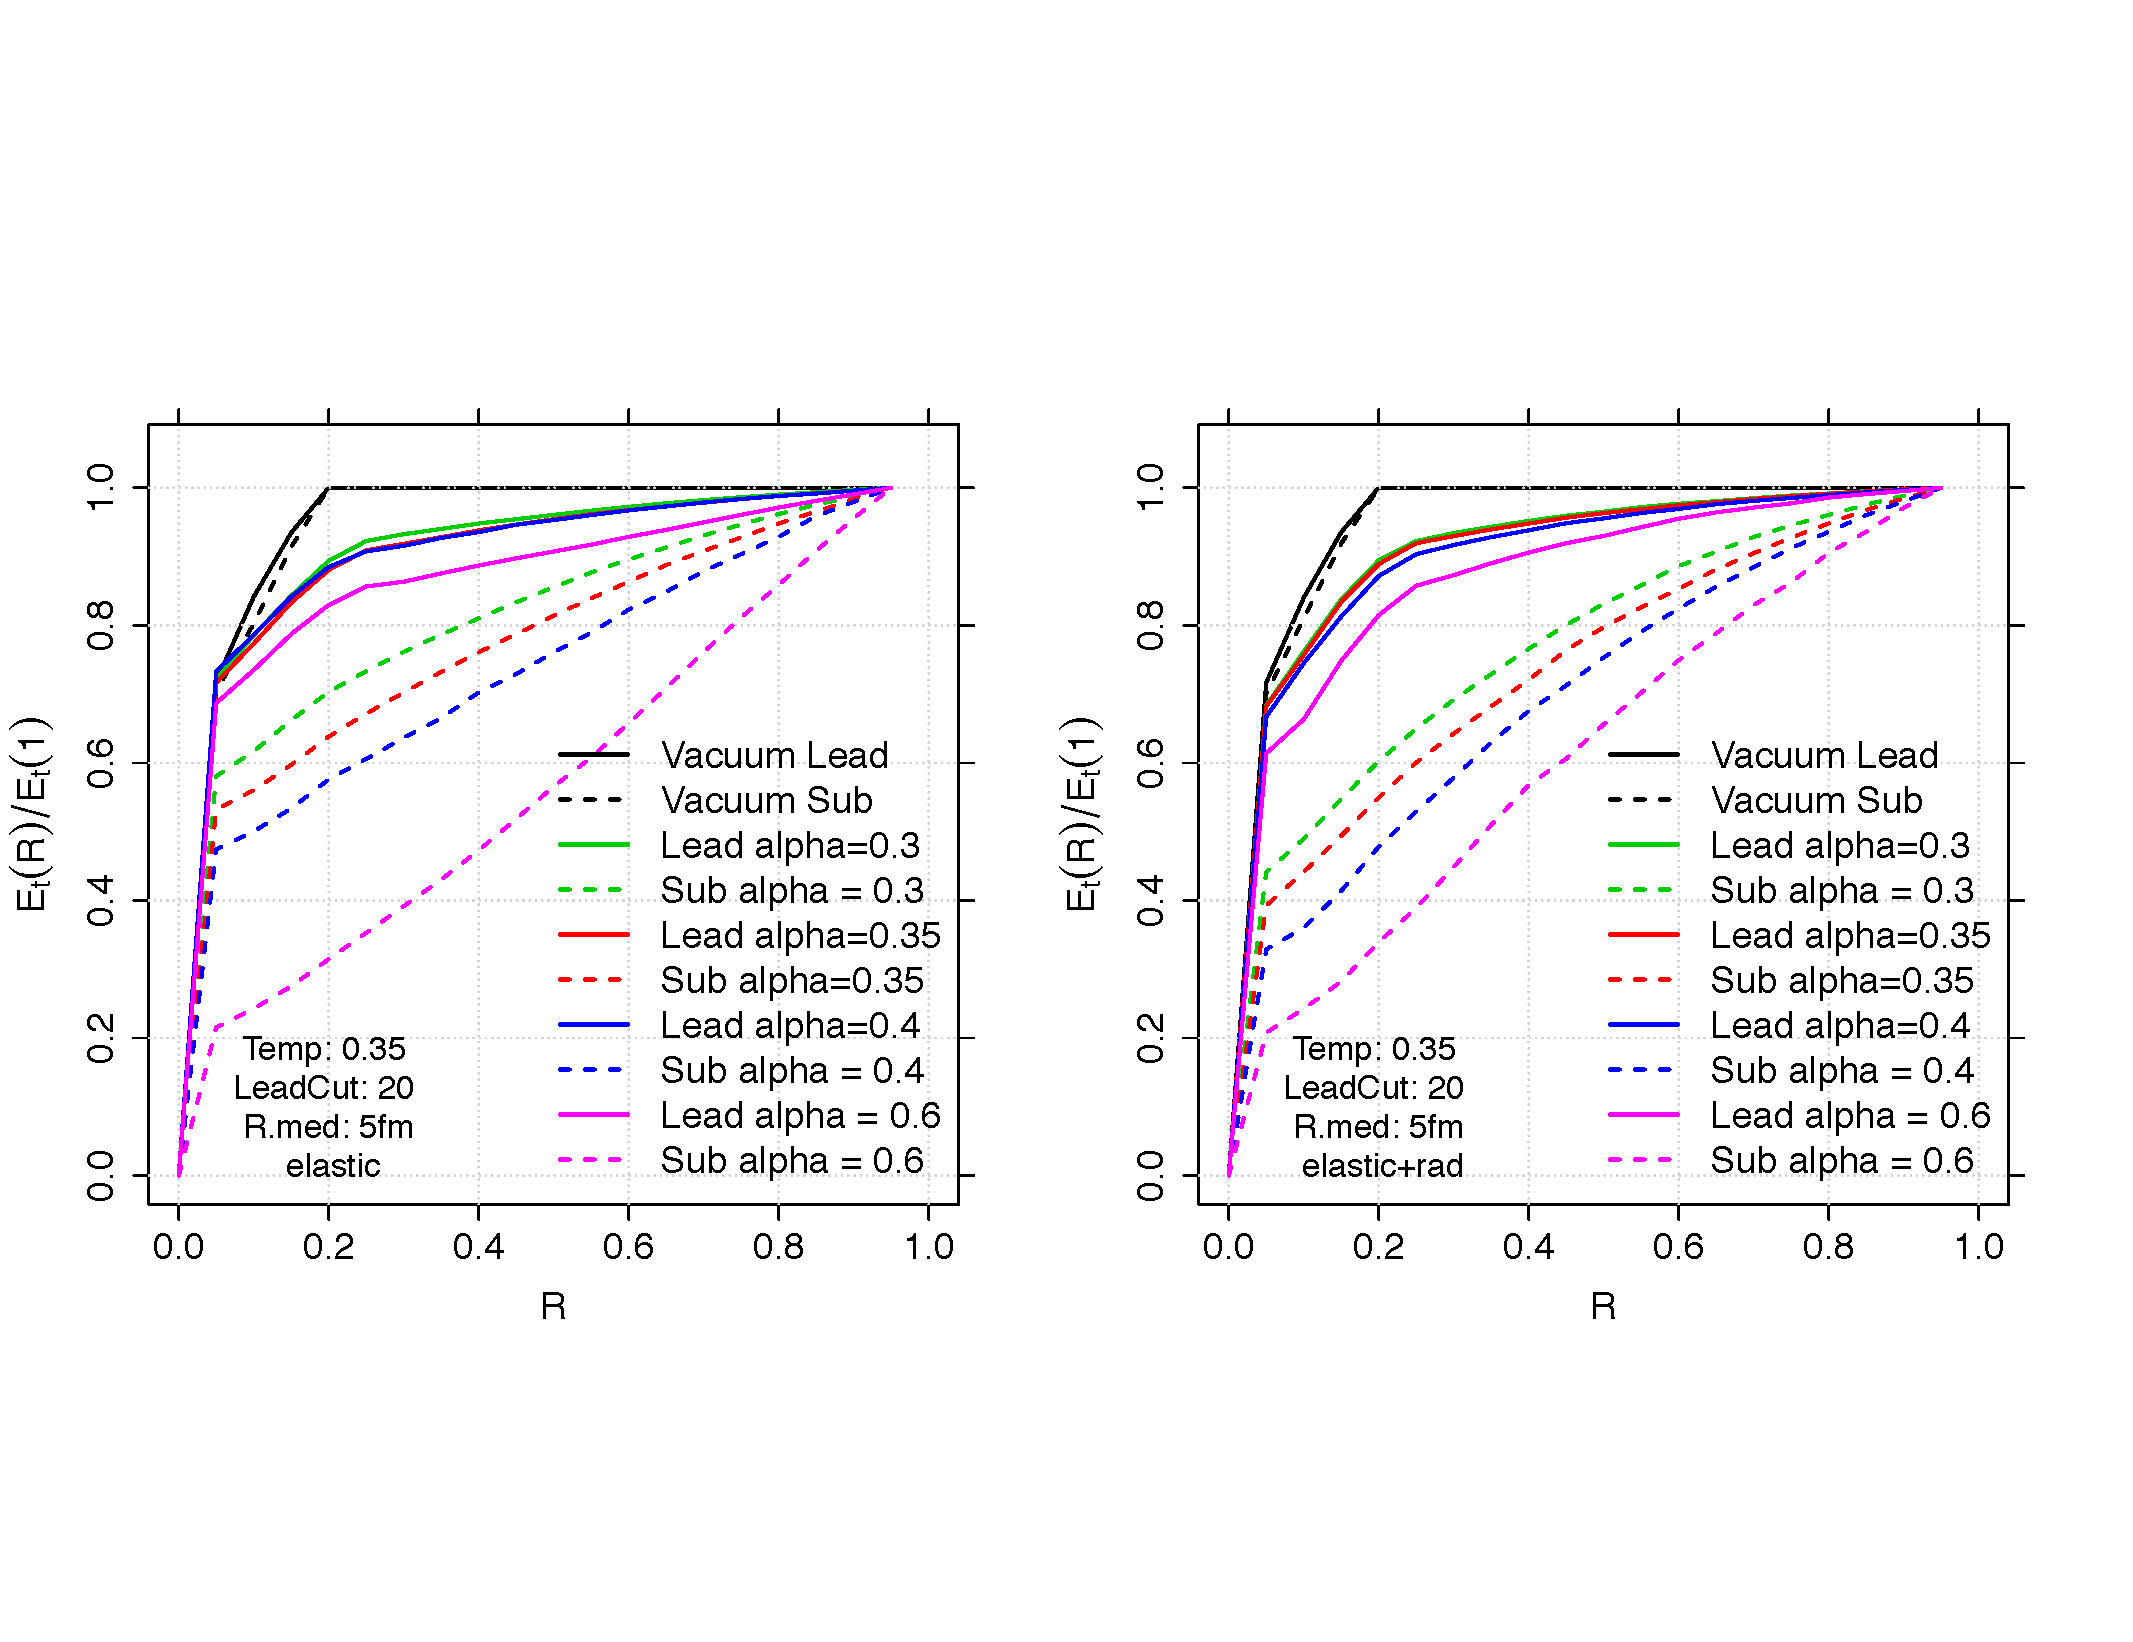
\includegraphics[trim = 505 2 15 2, clip,width=\textwidth]{figs/figure_physicscase_colemansmith_jetprofile}
%     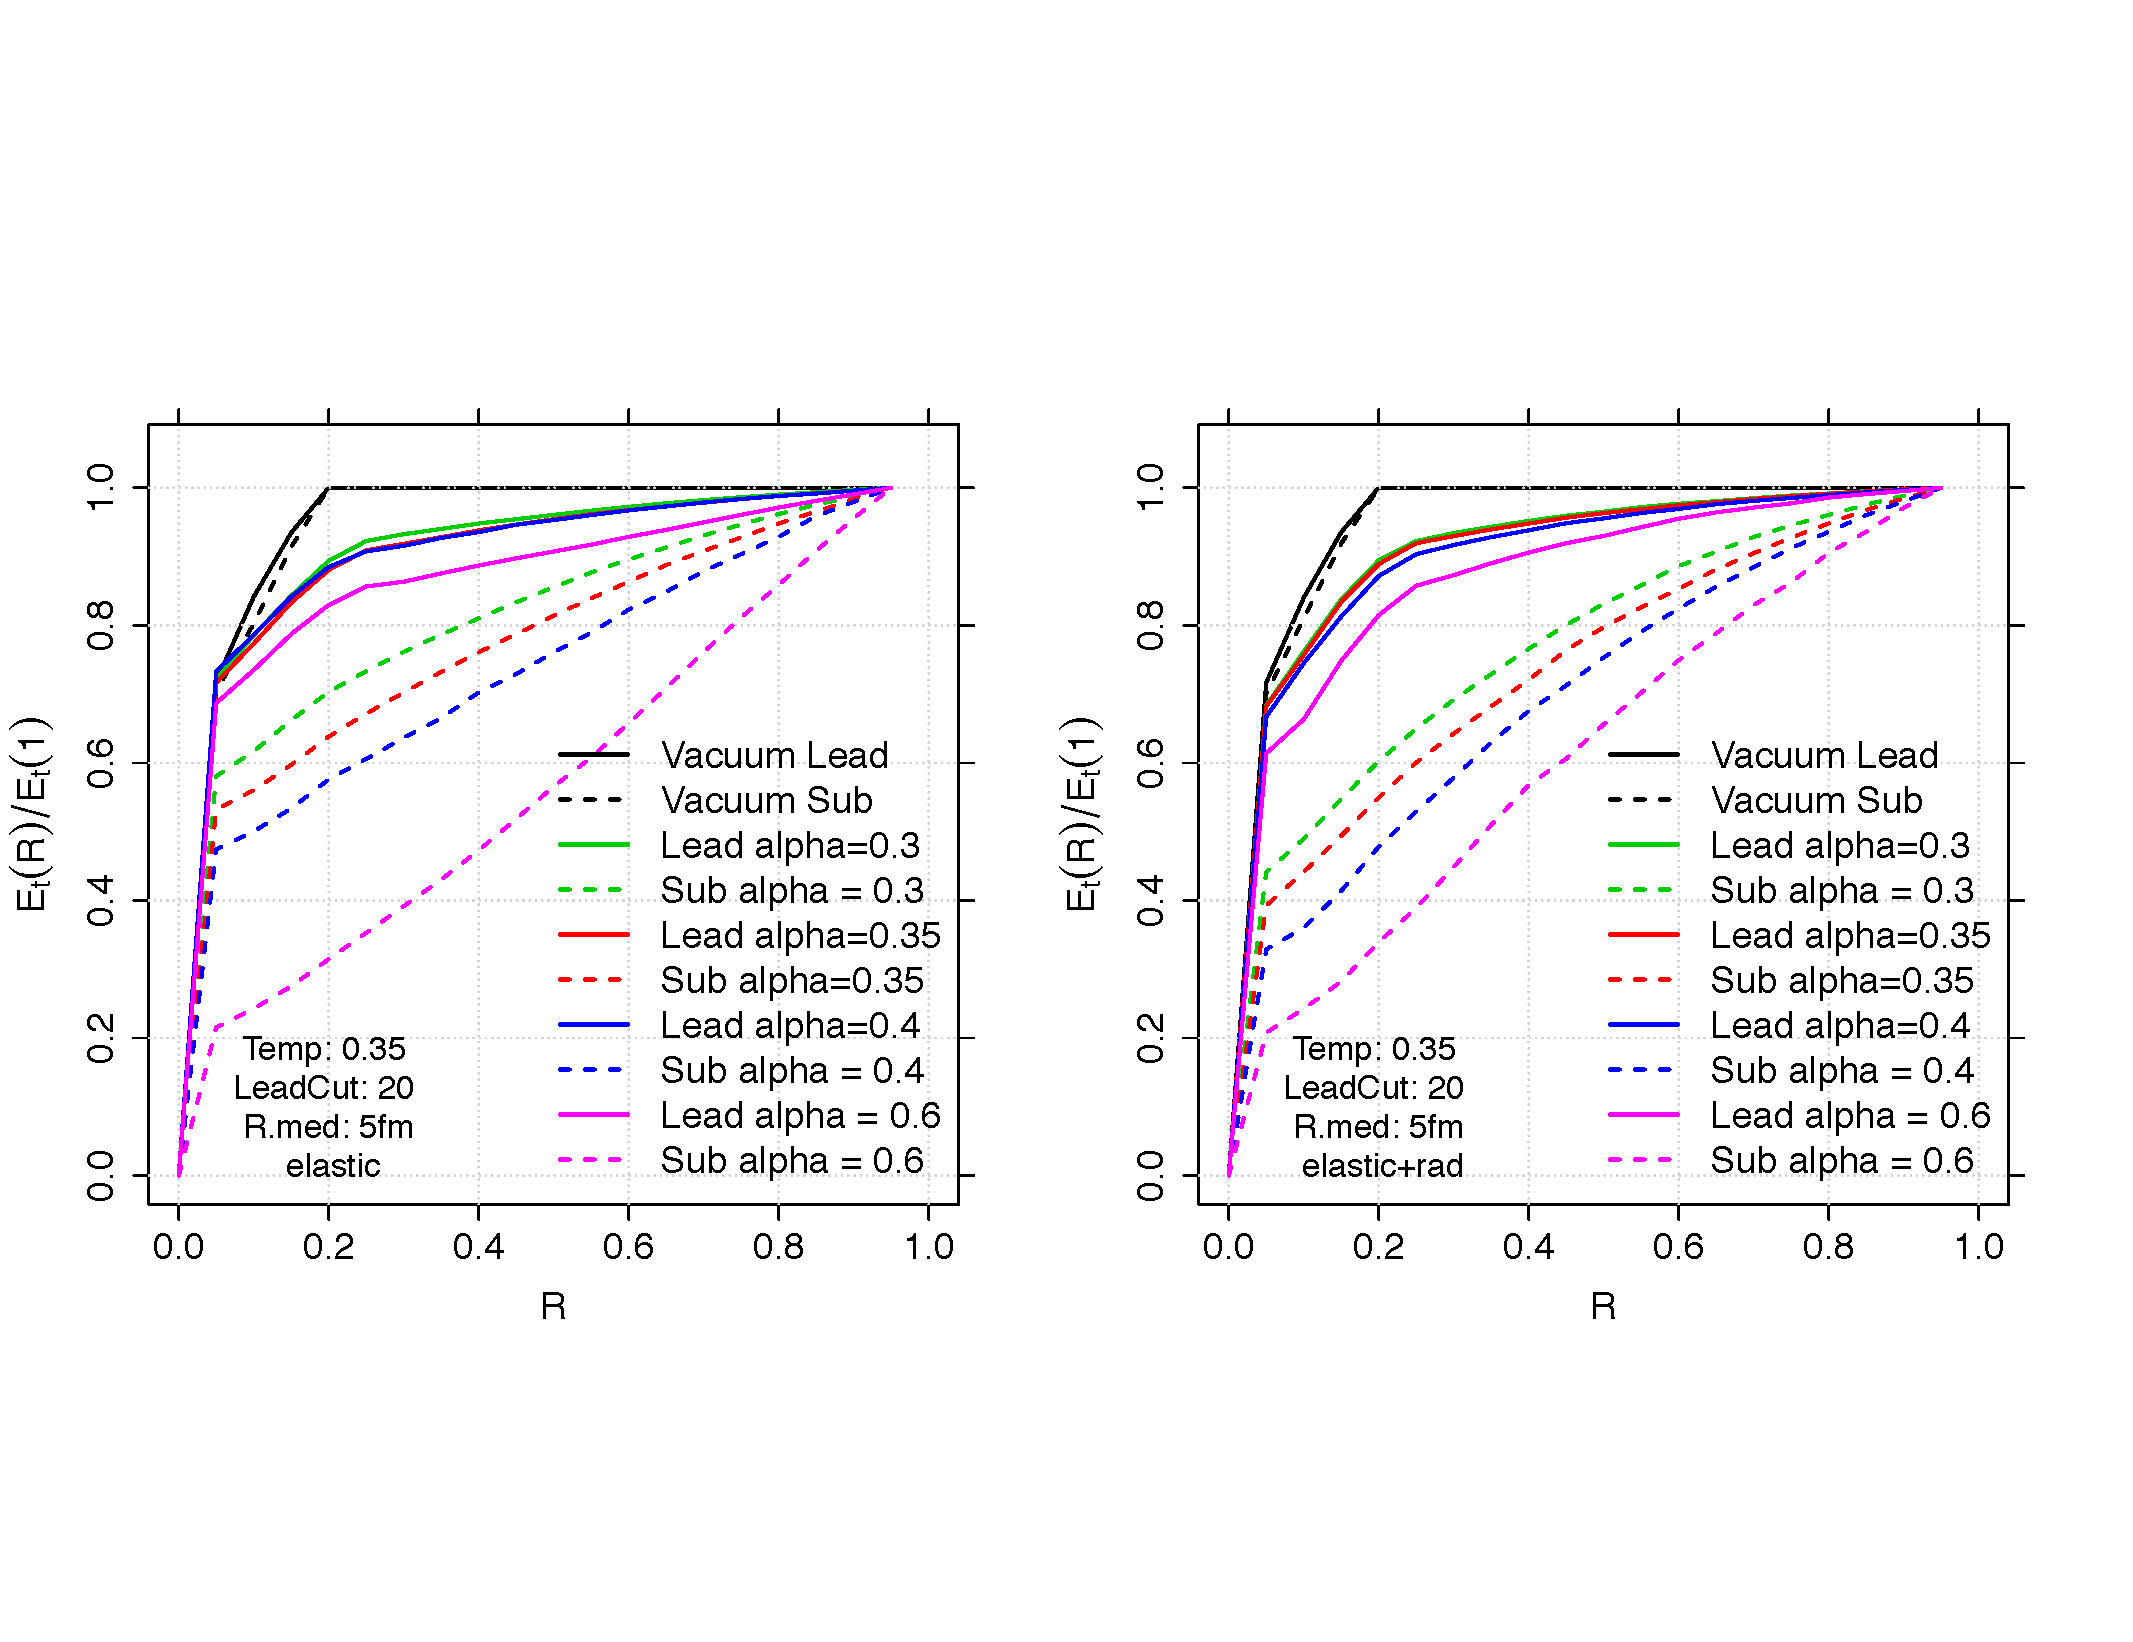
\includegraphics[trim = 2 2 520 2, clip,width=\textwidth]{figs/figure_physicscase_colemansmith_jetprofile}
%   \end{minipage}
%   \hfill
%   \raisebox{-0.3cm}{
%     \begin{minipage}[c]{0.71\textwidth}
%       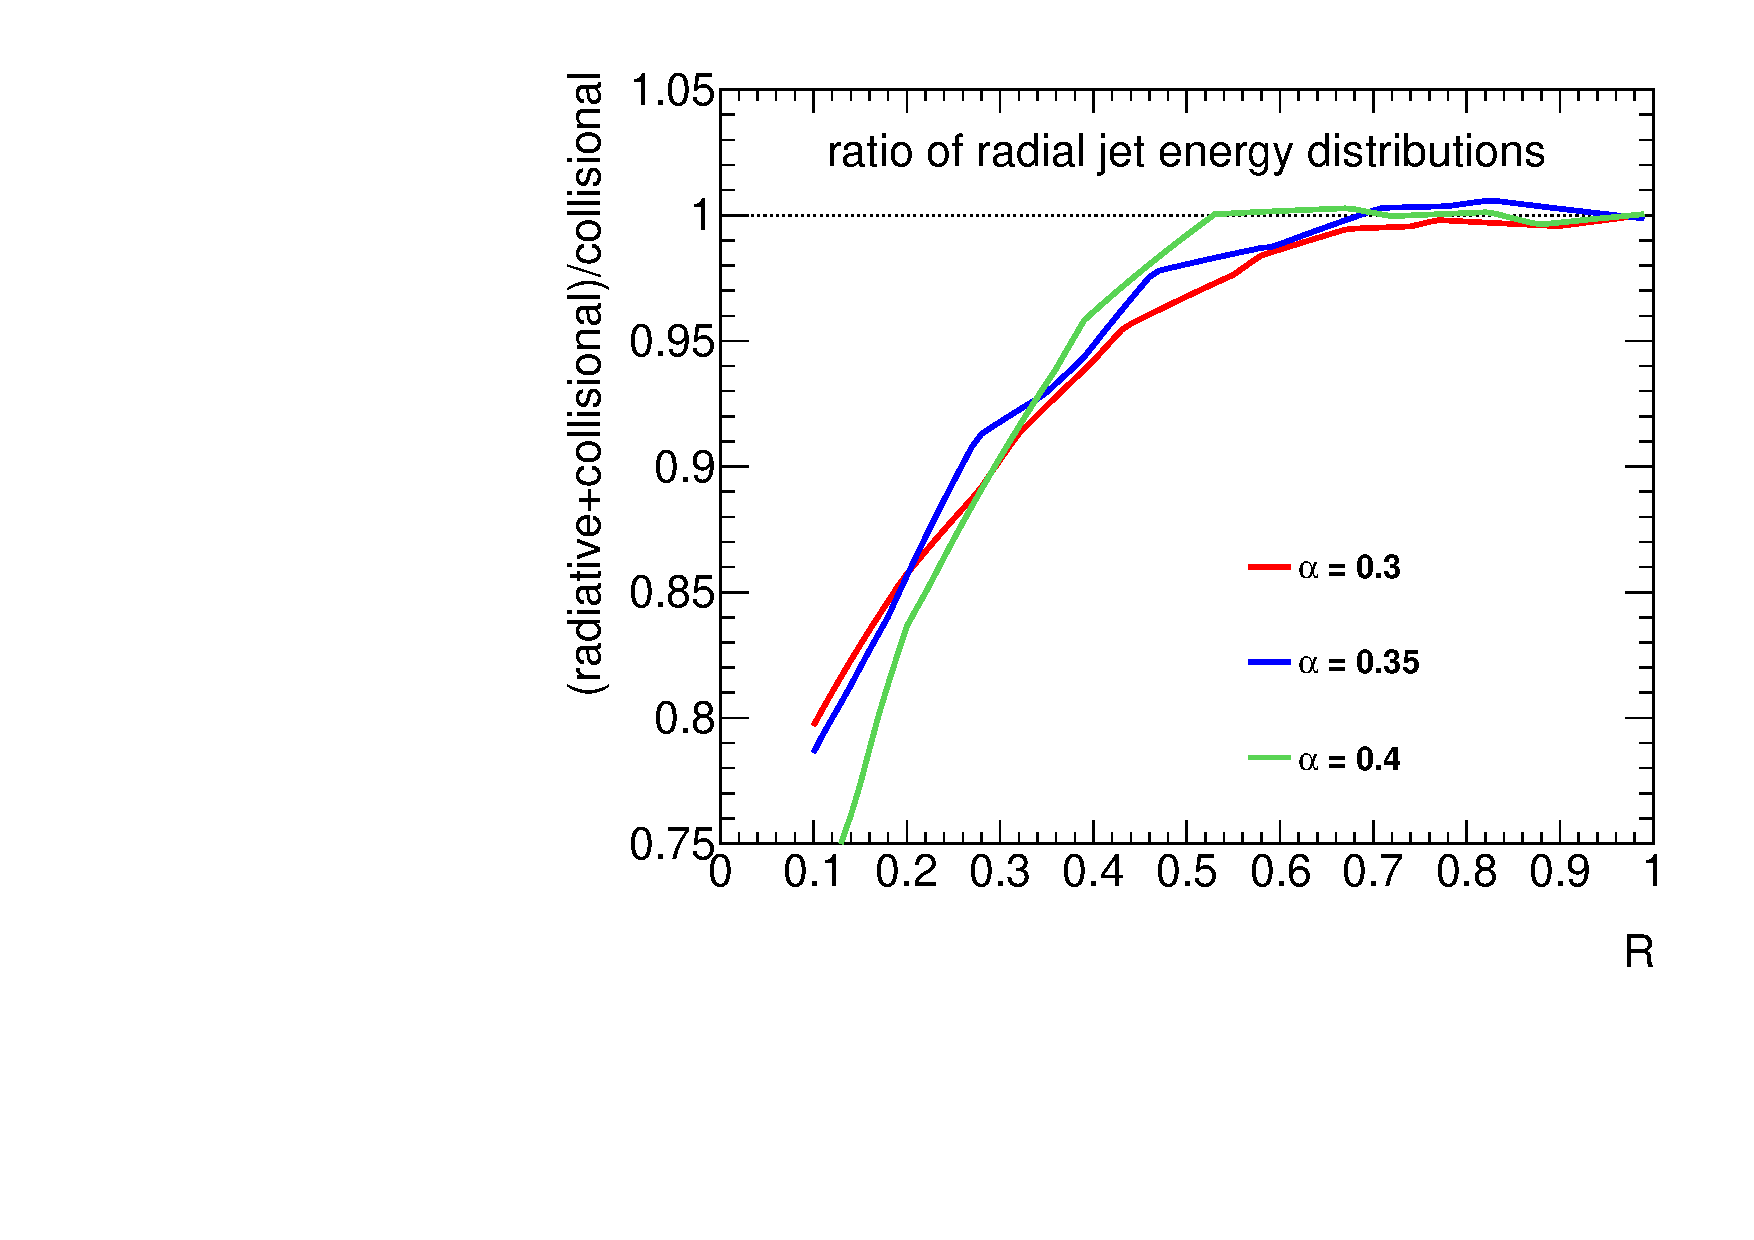
\includegraphics[width=\textwidth]{figs/colemansmith_jet_energy_ratio}
%     \end{minipage}
%   }
%   \caption[Calculations by Coleman-Smith of the jet energy profile as
%   a function of radius for leading and sub-leading
%   jets]{\label{fig:csjetprofile} (left) Calculations from
%     Coleman-Smith~\protect\cite{ColemanSmith:2012vr}{} showing the
%     jet energy profile as a function of radius for leading (solid
%     lines) and sub-leading (dashed lines) jets.  Leading jets have
%     $E_T>20$~GeV and sub-leading jets have $E_T>5$~GeV.  The medium
%     temperature is 350~MeV. (right) Ratio the radial distribution of
%     energy in sub-leading jets in a medium with radiative and elastic
%     energy loss to the distribution in a medium with elastic energy
%     loss only.  In these calculations, $\alpha$ serves as a proxy for
%     the effective medium coupling.  }
% \end{center}
%\end{figure}

%In the calculation by Vitev et
%al.~\cite{He:2011pd,Neufeld:2011yh,Vitev:2009rd}, the inclusion of
%collisional energy loss results in a substantial shift in the dijet
%asymmetry as shown comparing the top left and the bottom left of
%Figure~\ref{fig:vitevaj}.  The right panel of Figure~\ref{fig:vitevaj}
%shows the $A_{J}$ ratio with and without collisional energy loss.
%There is a significant additional suppression of back-to-back matched
%jets at low $A_{J}$ and a much larger number of very asymmetric jet
%pairs.  Detailed measurements as a function of jet energy, jet radius,
%and collision geometry are needed to map out the magnitude of the
%collisional component, and thus $\hat{e}$ and its related effective
%mass of the scattering centers.

%\begin{figure}[!hbt]
% \begin{center}
%%    \raisebox{0.02in}{\includegraphics[trim = 2 2 2 2, clip, width=\twowidth]{figs/figure_physicscase_vitev_aj_e30_r02}}
%%    \hfill
%%    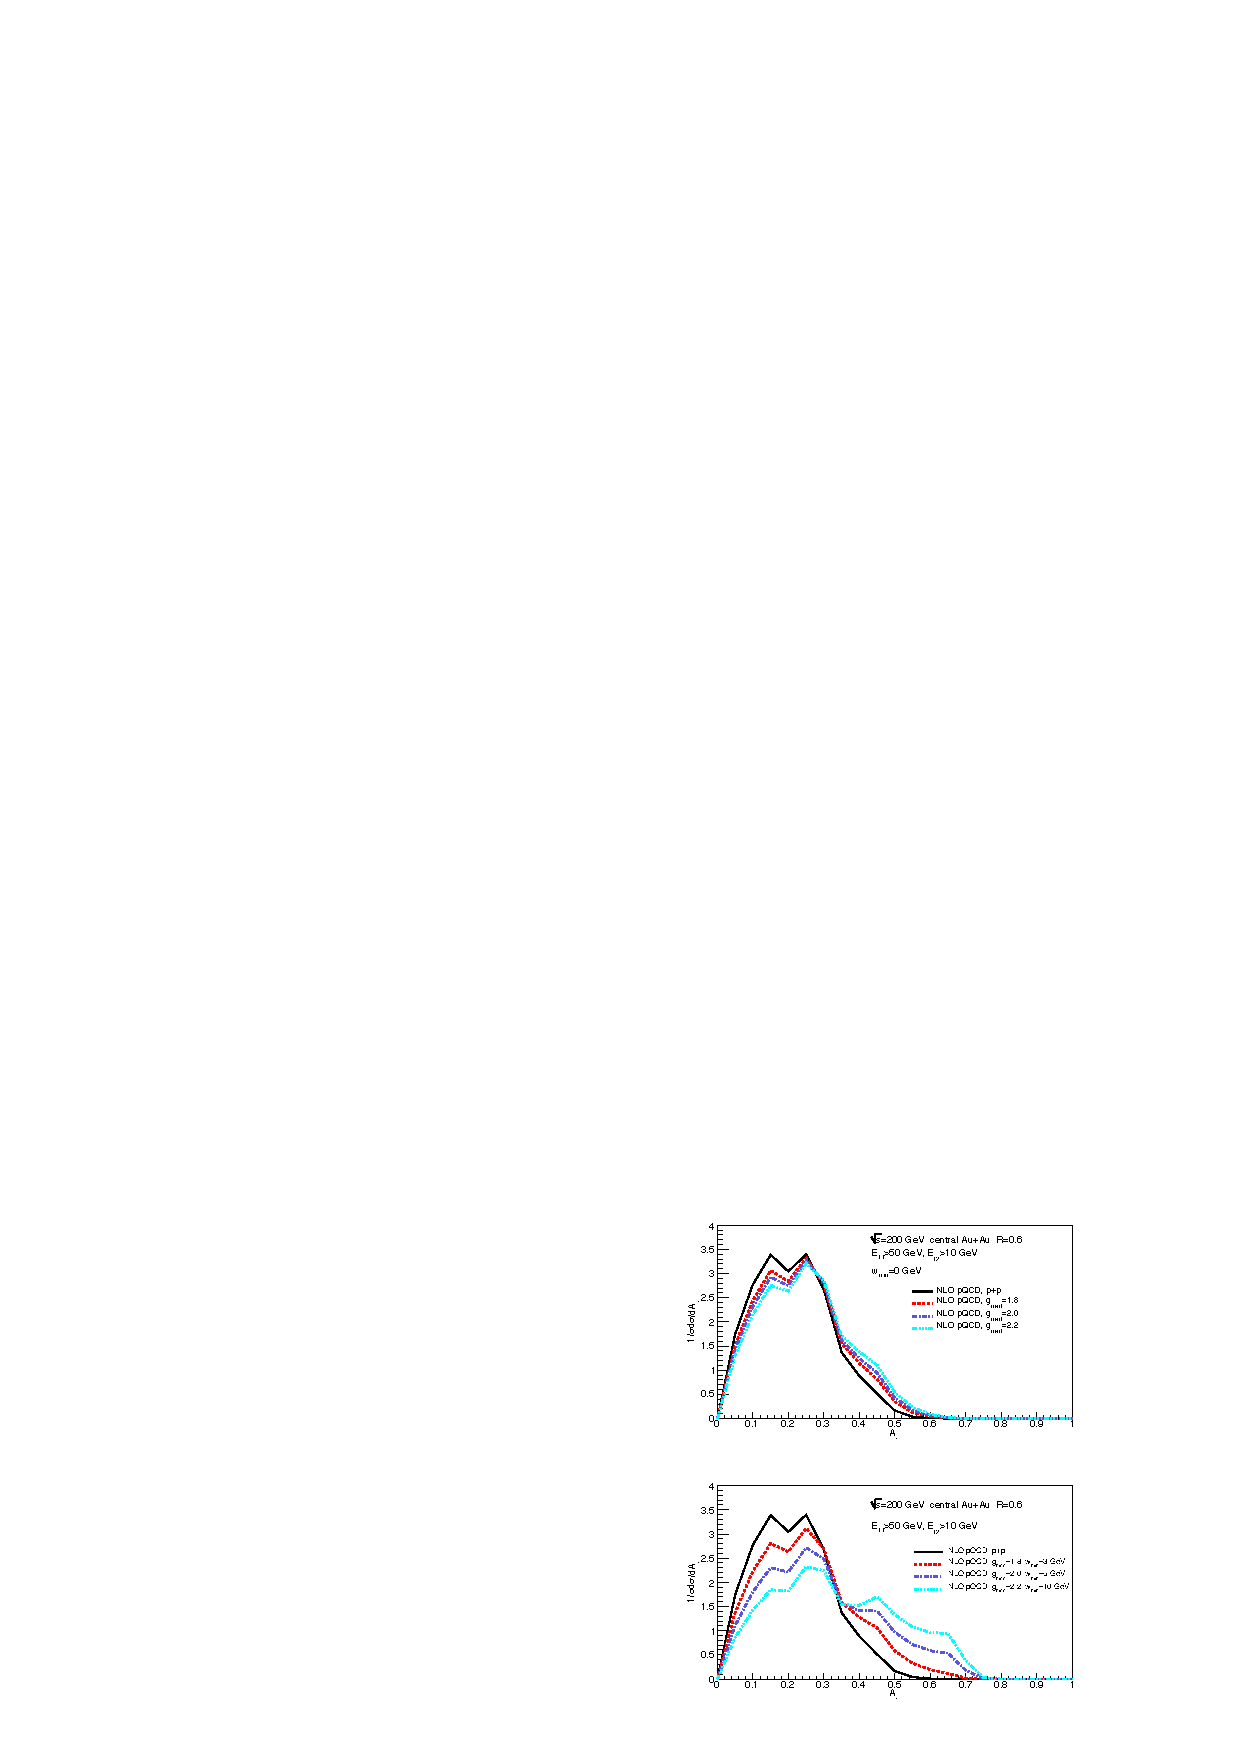
\includegraphics[trim = 2 2 2 2, clip,
%%    width=\twowidth]{figs/figure_physicscase_vitev_aj_e50}
%   \raisebox{0.55cm}{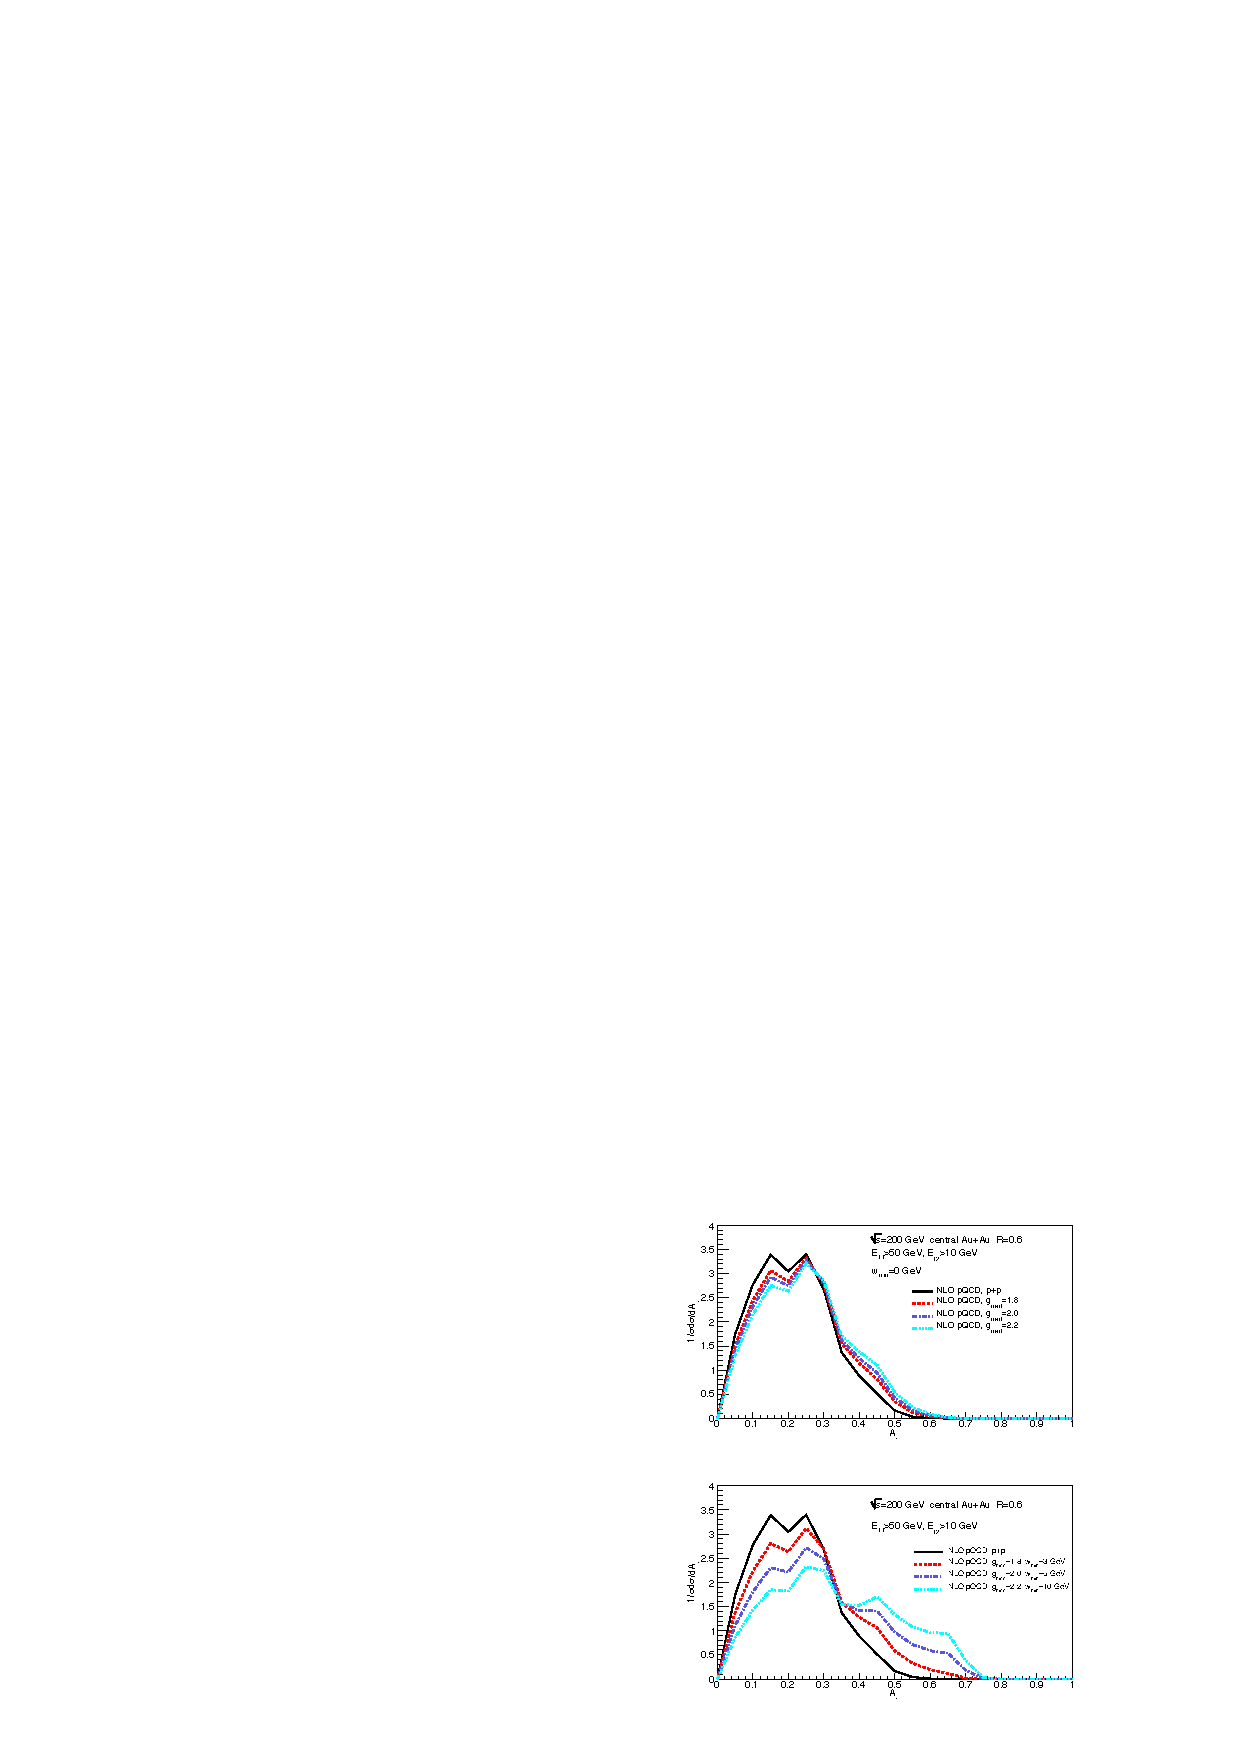
\includegraphics[trim = 2 2 2 2, clip, %width=0.35\textwidth]{figs/figure_physicscase_vitev_aj_e50}}
%   \hfill
%   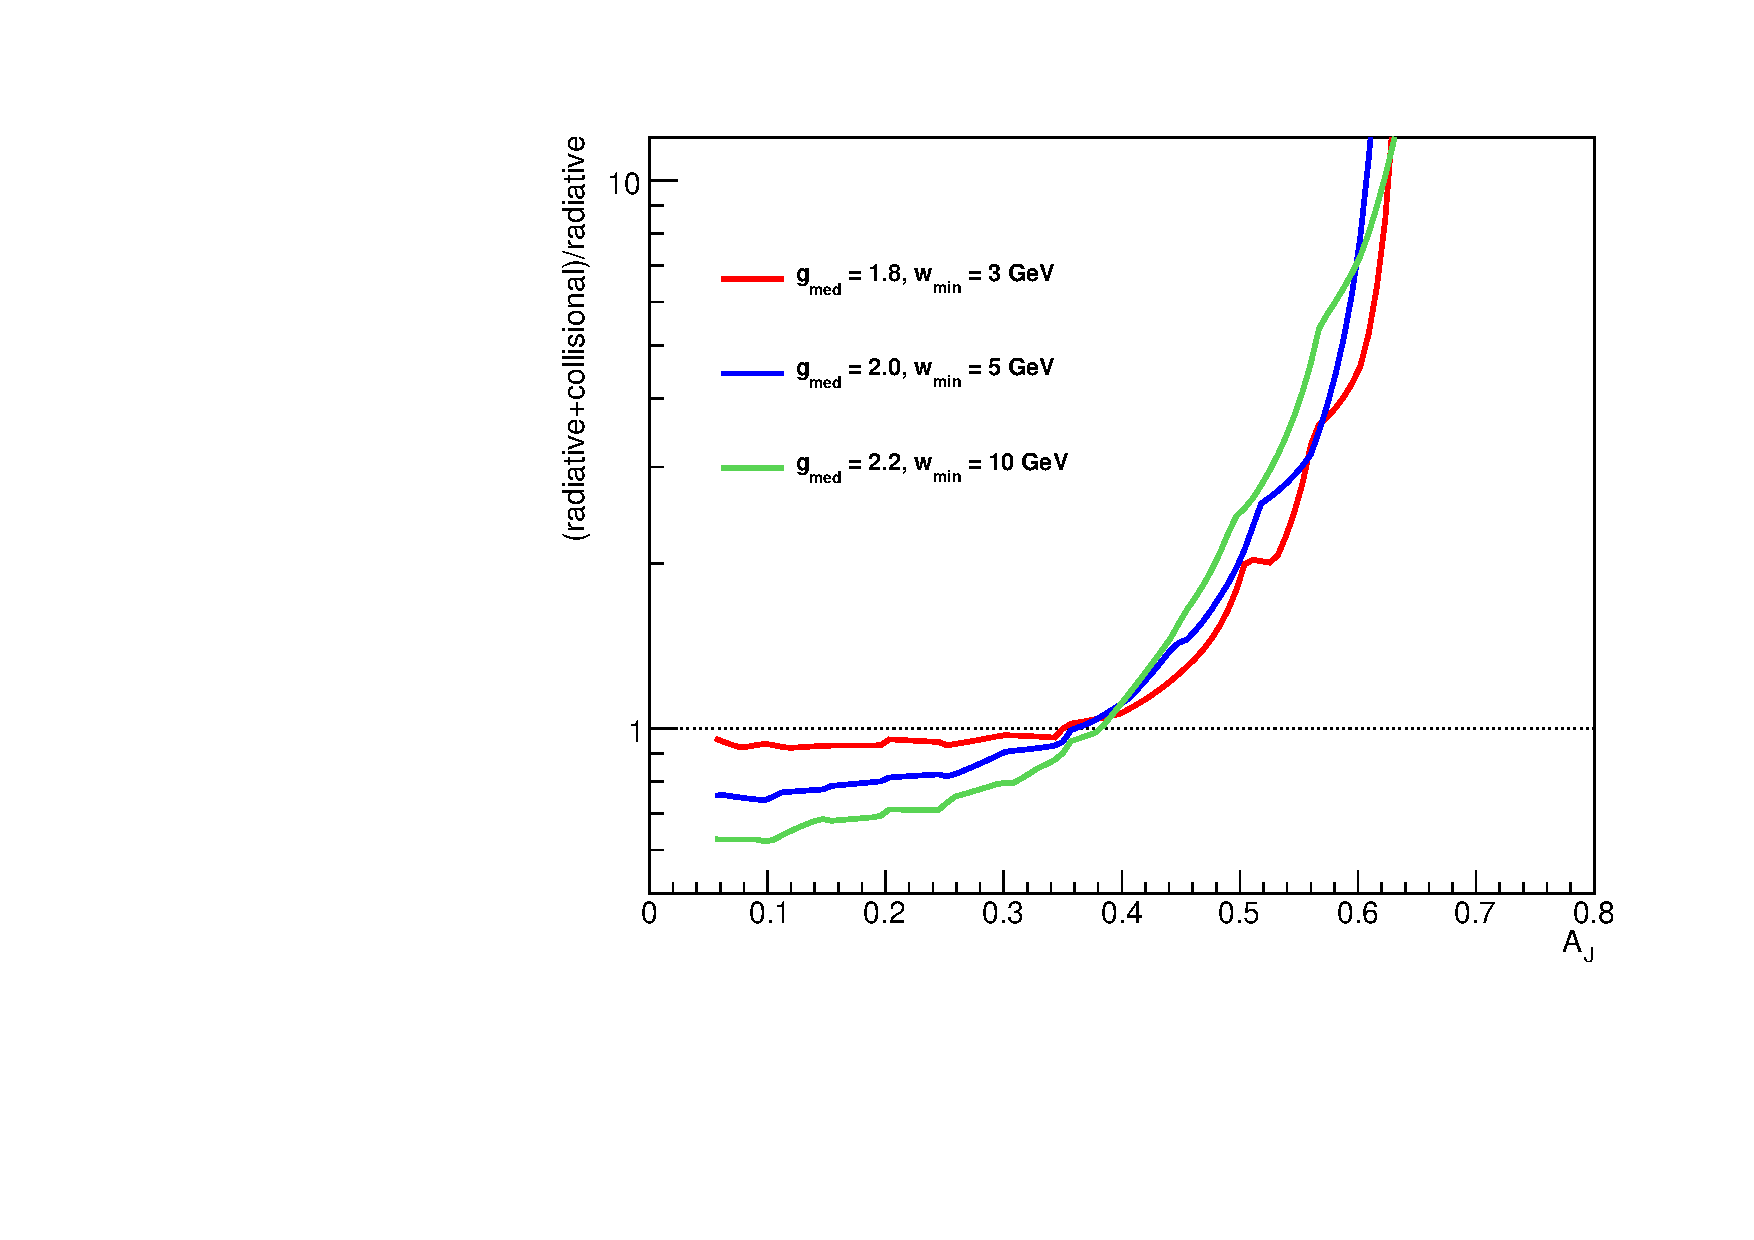
\includegraphics[width=0.62\textwidth]{figs/vitev_aj_modification.pdf}
%   \caption[$A_J$ distributions by Vitev et al. for leading jet $E_T >
%   50$~GeV, jet cone radius, $R = 0.6$, and different medium coupling
%   strengths]{\label{fig:vitevaj} (left) $A_J$ distributions
%     calculated by Vitev et
%     al.~\protect\cite{He:2011pd,Neufeld:2011yh,Vitev:2009rd}{} for
%     leading jet $E_T > 50$~GeV, jet cone radius, $R = 0.6$ and
%     different medium coupling strengths.  The upper plot shows
%     results for radiative energy loss only, and the lower plot
%     includes collisional energy loss as well. (right) Ratio of $A_J$
%     distributions with radiative and collisional energy loss to those
%     with radiative energy loss only.}
% \end{center}
%\end{figure}

%One of the most sensitive observables to collisional energy loss is the modification of high \pt charm
%and beauty heavy quarks in the medium.   We detail this physics in the later section specifically
%on heavy quarks -- Section~\ref{sec:heavyquark}.

%\clearpage

\section{How does the QGP evolve along with the parton shower?}
\label{sec:medium_evolution}

The initial hard scattered parton starts out very far off-shell and in
$e^{+}e^{-}$, \pp or \ppbar~collisions the virtuality evolves in
vacuum through gluon splitting down to the scale of hadronization.  In
heavy ion collisions, the vacuum virtuality evolution is interrupted
at some scale by scattering with the medium partons which increase the
virtuality with respect to the vacuum evolution.
Figure~\ref{fig:virtualityevolution} shows the expected evolution of
virtuality in vacuum, from medium contributions, and combined for a
quark-gluon plasma at $T_0 = 300$~MeV with the traversal of a 30~GeV
parton (left) and at $T_{0}=390$~MeV with the traversal of a 200~GeV
parton (right)~\cite{Muller:usersmeeting,Muller:2010pm}.  If this
picture is borne out, it ``means that the very energetic parton [in
the right picture] hardly notices the medium for the first 3--4 fm of
its path length~\cite{Muller:2010pm}.'' Spanning the largest possible
range of virtuality (initial hard process $Q^{2}$) is very important,
but complementary measurements at both RHIC and LHC of produced jets
at the same virtuality (around 50~GeV) will test the interplay between
the vacuum shower and medium scattering contributions.

\begin{figure}[!hb]
 \begin{center}
    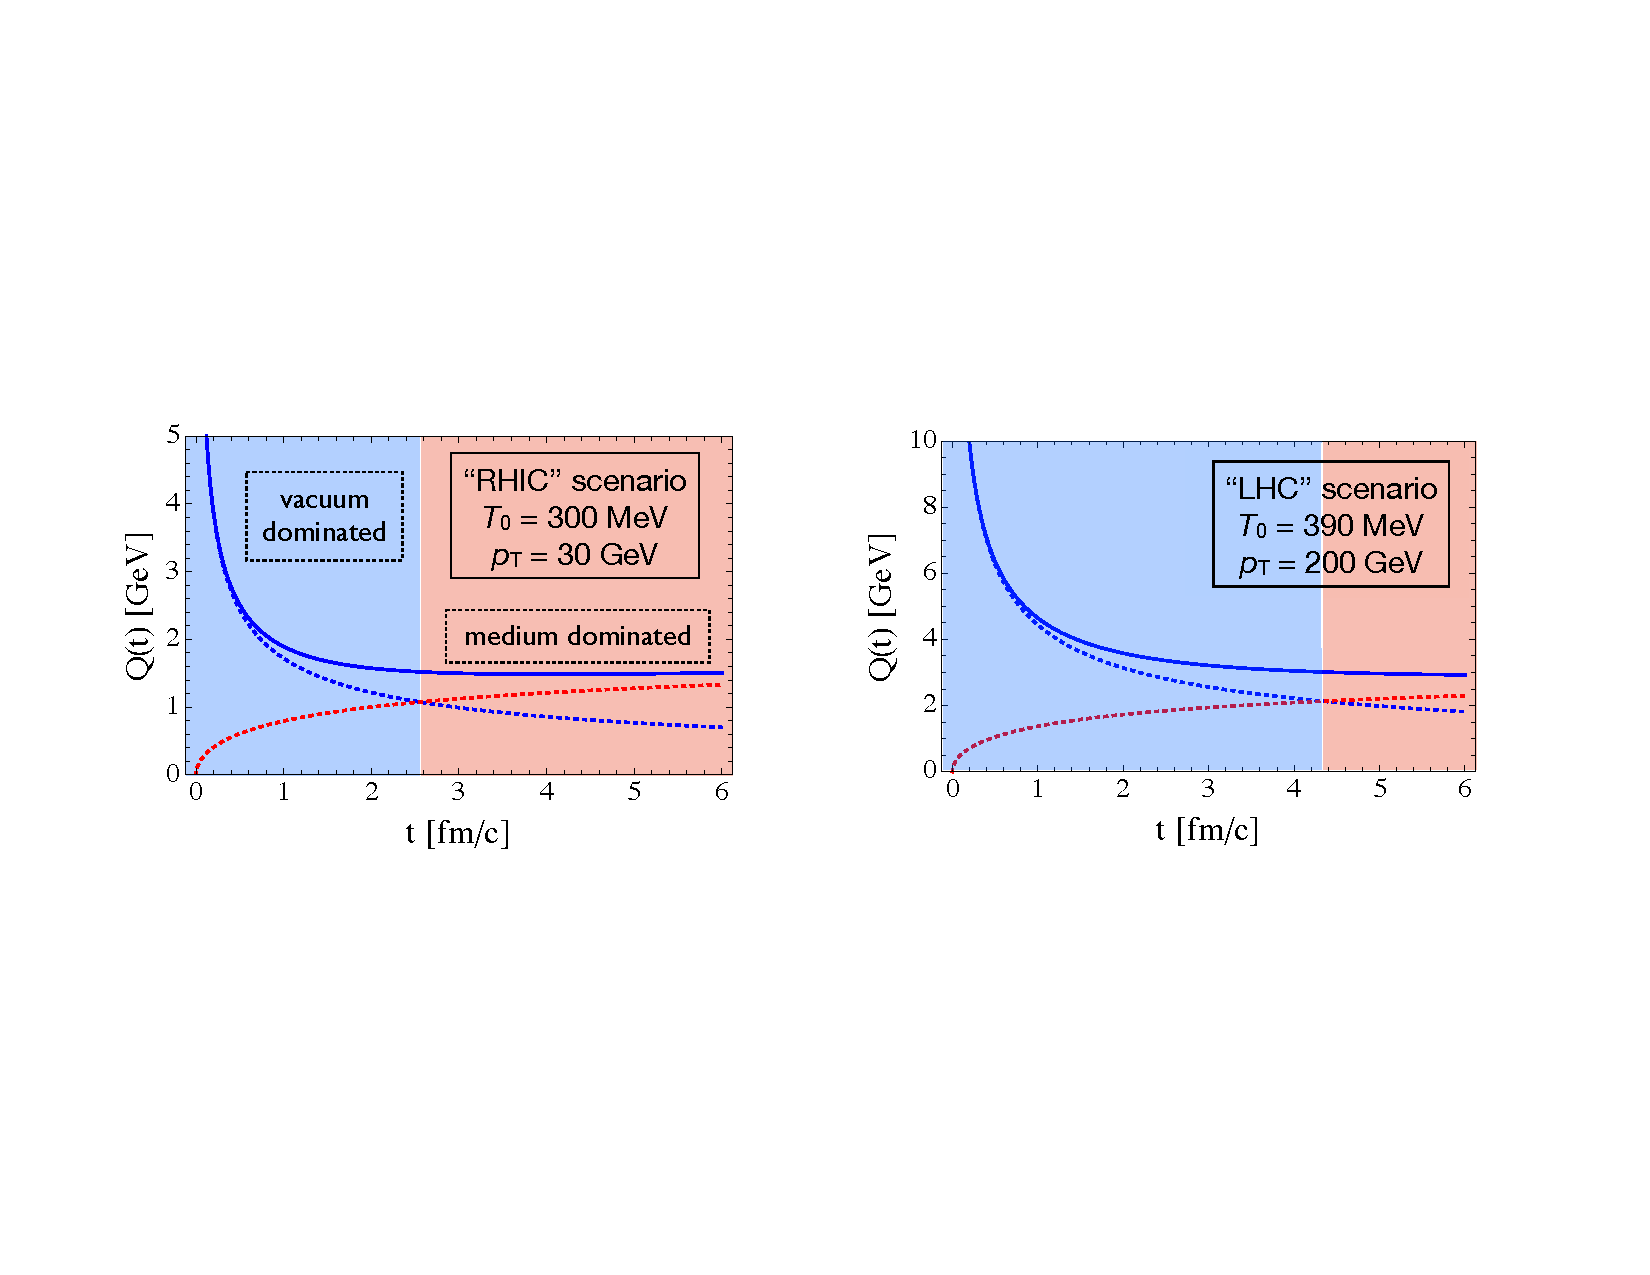
\includegraphics[trim = 2 2 2 2, clip, width=0.95\linewidth]{figs/figure_physicscase_virtualityevolution}
    \caption[Jet virtuality evolution in medium at RHIC and
    LHC]{\label{fig:virtualityevolution}Jet virtuality evolution in
      medium at RHIC (left) and LHC (right).  Vacuum contributions to
      virtuality (blue dashed lines) decrease with time and medium
      induced contributions (red dashed lines) increase as the parton
      scatters in the medium.  The total virtuality (blue solid lines)
      is the quadrature sum of the two contributions.  At RHIC the
      medium induced virtuality dominates by 2.5\,fm/c while at the
      LHC the medium term does not dominate until 4.5\,fm/c.  From
      Ref.~\protect\cite{Muller:usersmeeting}{}.}
 \end{center}
\end{figure}

In some theoretical frameworks --- for example
Refs~\cite{Renk:2013rla,Majumder:2011uk,Majumder:2014gda} --- the
parton splitting is simply dictated by the virtuality and in vacuum
this evolves relatively quickly from large to small scales as shown
above.  The $Q$ evolution means that the jet starts out being
considerably off mass shell when produced, and this off-shellness is
reduced by successive splits to less virtual partons.  In these
calculations, the scattering with the medium modifies this process of
parton splitting.  The scale of the medium as it relates to a
particular parton is $\hat{q}$ times the parton lifetime (this is the
mean transverse momentum that the medium may impart to the parent and
daughter partons during the splitting process). When the parton's
off-shellness is much larger than this scale, the effect of the medium
on this splitting process is minimal. As the parton drops down to a
lower scale, the medium begins to affect the parton splitting more
strongly.

Shown in Figure~\ref{fig:virtualityevolution_singlehadron} is the
single hadron \raa in central \auau collisions at 200~GeV along
side measurements at other beam energies.  One specifically notes that
for the YAJEM calculation, inclusion of the virtuality evolution leads
to a factor of 50\% rise in \raa from 20--40~GeV/c, and in the HT-M
calculation a 100\% rise. A strong rise in \raa measured at
higher \pt at the LHC has been observed, and measurement of the
consistent effect within the same framework at RHIC is a key test of
this virtuality evolution description. It is notable that the JEWEL
calculation which describes the rising \raa at the
LHC~\cite{Zapp:2013vla}, results in a nearly flat \raa over the entire
\pt range at RHIC. sPHENIX can perform precision measurements of
charged hadrons over this \pt range.

\begin{figure}[!hbt]
 \begin{center}
   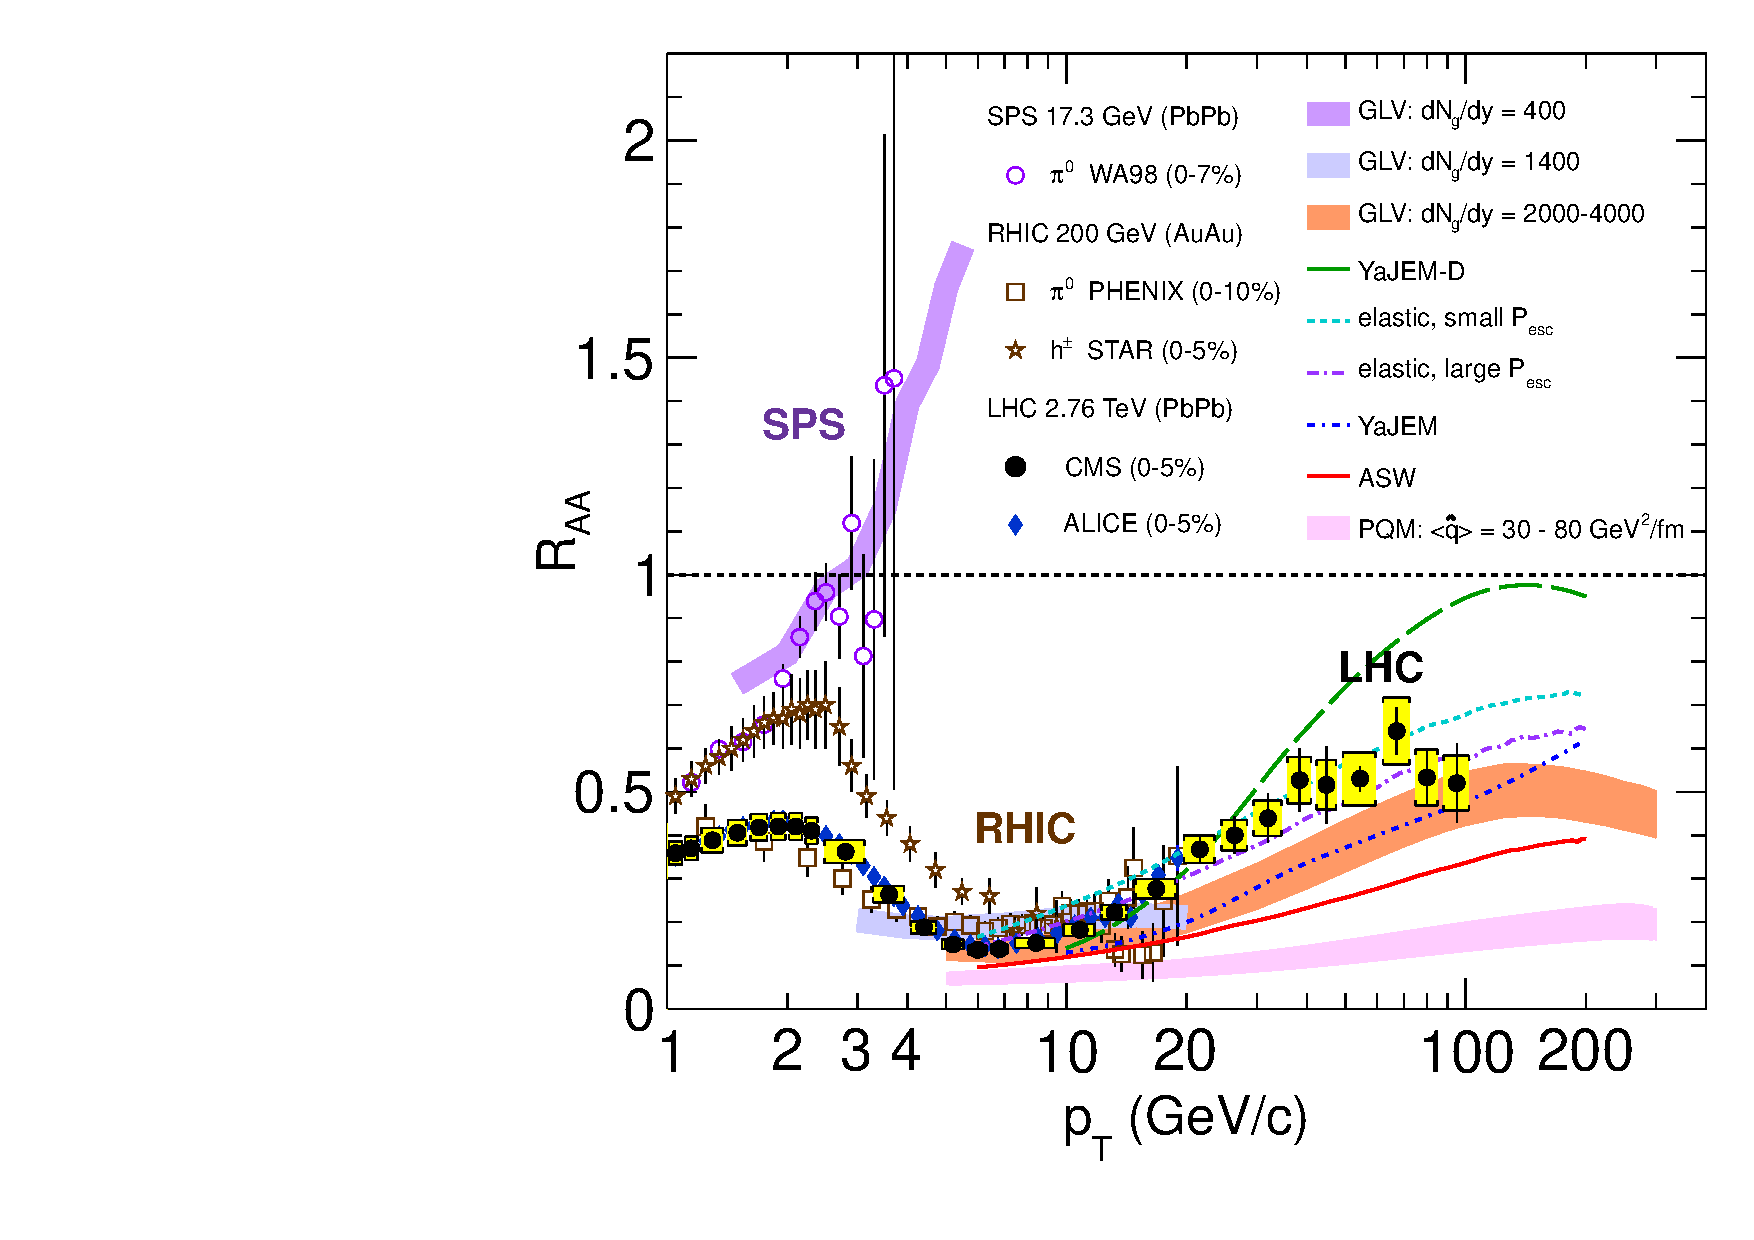
\includegraphics[width=0.43\linewidth]{figs/raa_compiled_QM11_square_hi2011}
   \raisebox{0.33cm}{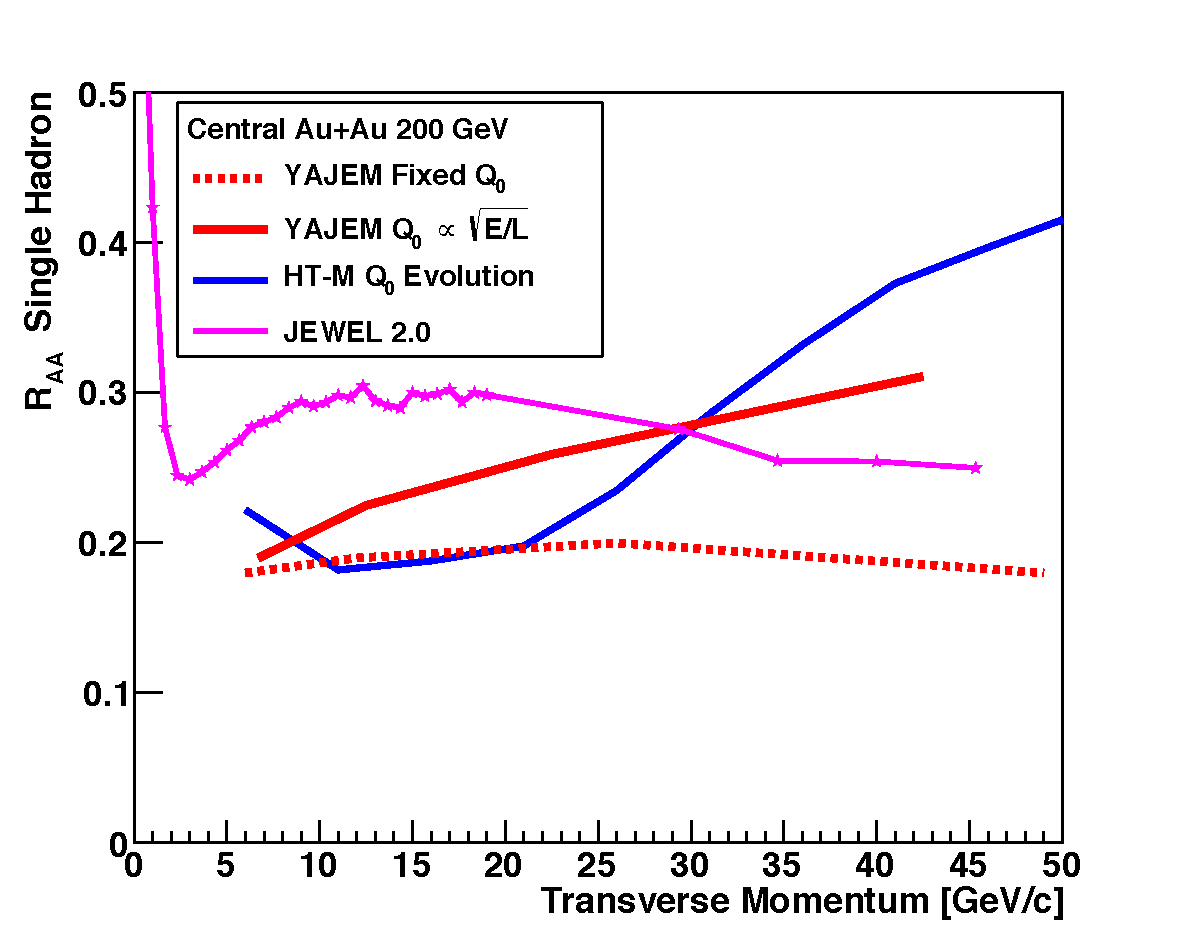
\includegraphics[width=0.55\linewidth]{figs/figure_rhic_pizeroraa_q0evol}}
   \caption[ The nuclear modification factor \raa vs transverse
   momentum at the SPS, RHIC, and LHC, compared to various jet
   quenching calculations]{(left) The nuclear modification factor \raa
     as a function of transverse momentum in A$+$A collisions at the
     SPS, RHIC, and LHC.  Comparisons with various jet quenching
     calculations as detailed in Ref.~\cite{CMS:2012aa} and references
     therein are shown.  The simultaneous constraint of RHIC and LHC
     data is a powerful discriminator. (right) Predictions for single
     hadrons \raa to $\pT\sim50$~GeV/$c$ in central \auau at 200~GeV.}
  \label{fig:virtualityevolution_singlehadron}
  \label{fig:cmsqhat}
 \end{center}
\end{figure}

%Further emphasizing the importance of having such measurements over the maximum kinematic reach at RHIC
%and the LHC are the recent jet and charged hadron $R_{pA}$ measurements shown in Figure~\ref{fig:cms_raa}.  
%It is quite striking that the flat reconstructed jet \raa and rising charged hadron \raa are mimicked already
%in proton-nucleus collisions.   This may hint that all the physics of the rising hadron \raa does not fully
%constrain the virtuality evolution and various calculations thus predict quite different effects at RHIC.

%\begin{figure}[!hbt]
% \begin{center}
%   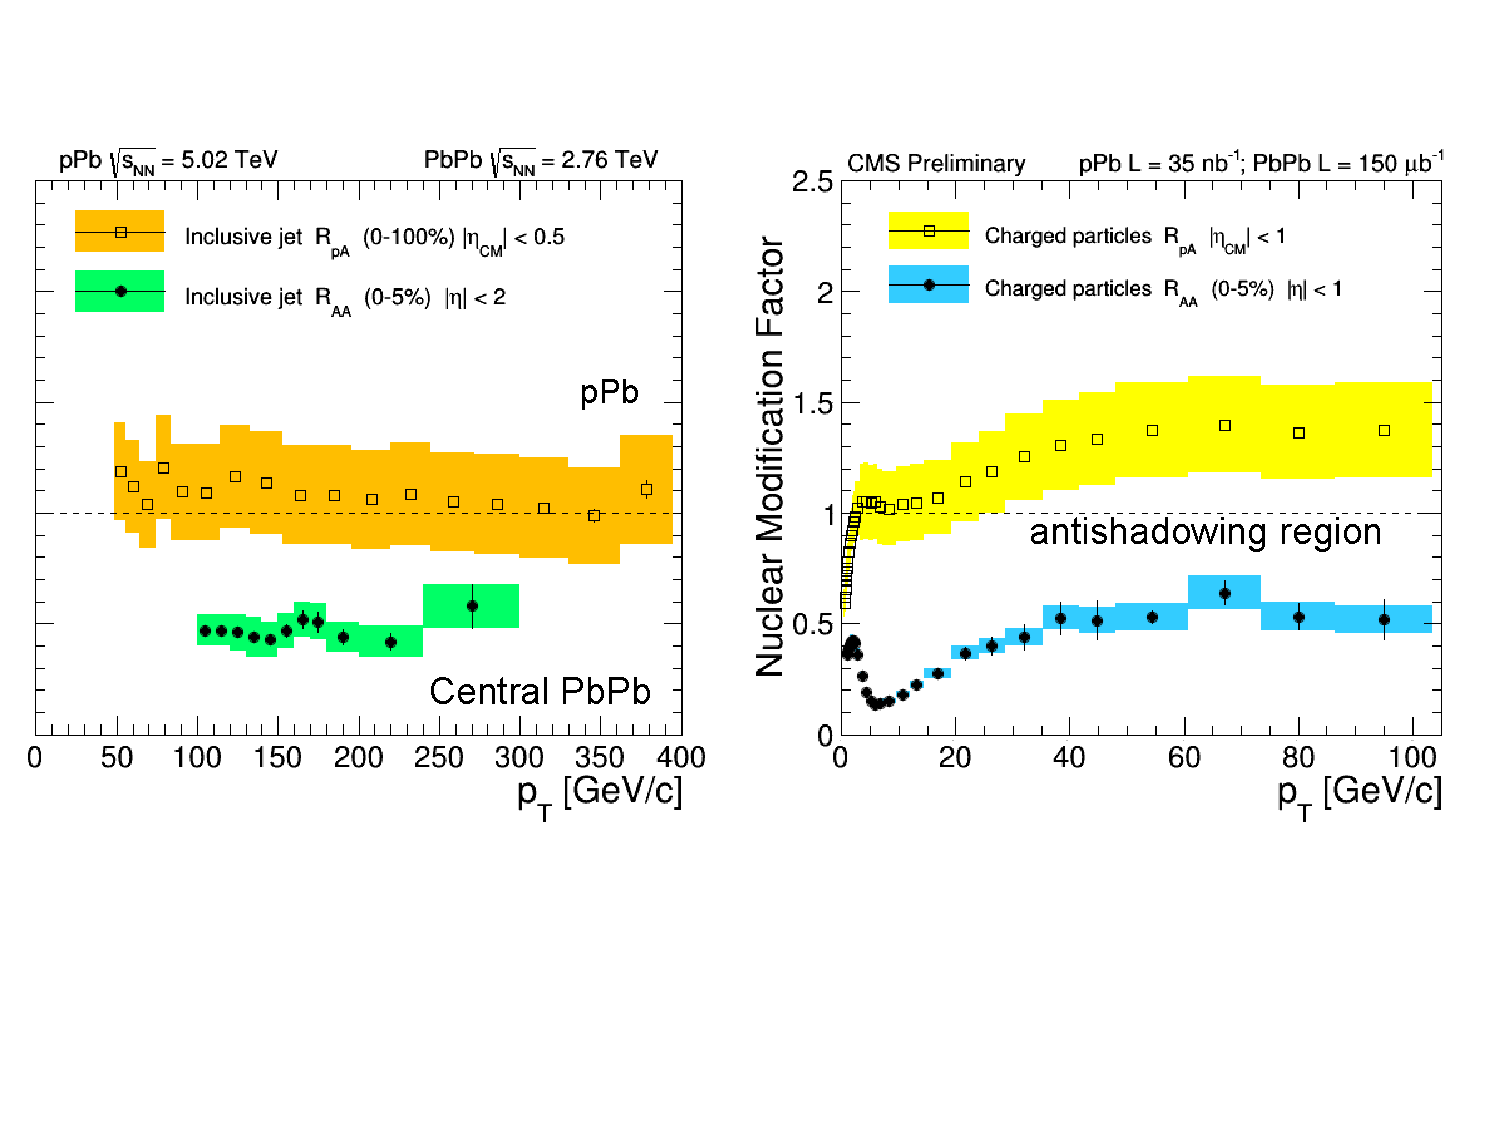
\includegraphics[width=0.95\linewidth]{figs/CMS_raa_jets_hadrons}
%   \caption[Preliminary CMS results of jet and charged particle \raa
%   in \pA and \pbpb]{(left) Preliminary results from CMS showing the
%     jet \raa in \pA near 1 and in \pbpb near 0.2. (right) Preliminary
%     results from CMS showing the charged particle \raa in \pA and in
%     \pbpb.  In contrast to the jet \raa results which are essentially
%     flat with \pT, the charged particle \raa shows a rise with \pT.}
%  \label{fig:cms_raa}
% \end{center}
%\end{figure}

To convey the scale probed and virtuality evolution differences at
RHIC and the LHC, we show the off-shellness of the initial hard
scattered parton virtuality in units of 1/fm as a function of the local temperature of
the QGP medium where the parton resides in Figure~\ref{fig:magic2}.  The calculation incorporates
the vacuum virtuality evolution which falls off quickly with time and
the medium scattering contribution that kicks the virtuality back up.
We incorporate the full time evolution of pre-equilibrium dynamics,
viscous hydrodynamics, and hadron cascade from
Ref.~\cite{Habich:2014jna} to map the time of the parton evolution to
the local temperature.  The medium virtuality contribution also scales
with the local temperature. The red (black) curves are for
different initial parton energies in the RHIC (LHC) medium.  The
thicker line regions highlight where the medium virtuality has a
substantial influence on the parton splitting.  It is notable that
highest energy partons at the LHC, of order 1 TeV, are always
dominated by the initial vacuum virtuality evolution (for more than 10
fm/c).  In contrast, the lower energy jets and the RHIC medium
evolution have the largest influence and map out a unique part of this
microscope resolving power and temperature of the \qgp.

THE FIGURE BELOW MIGHT BE REMOVED AND JUST REFER TO THE VIRTUALITY EVOLUTION FIGURE THAT WAS PART OF THE NSAC LRP SIDEBAR.

\begin{figure}[!hbt]
 \begin{center}
   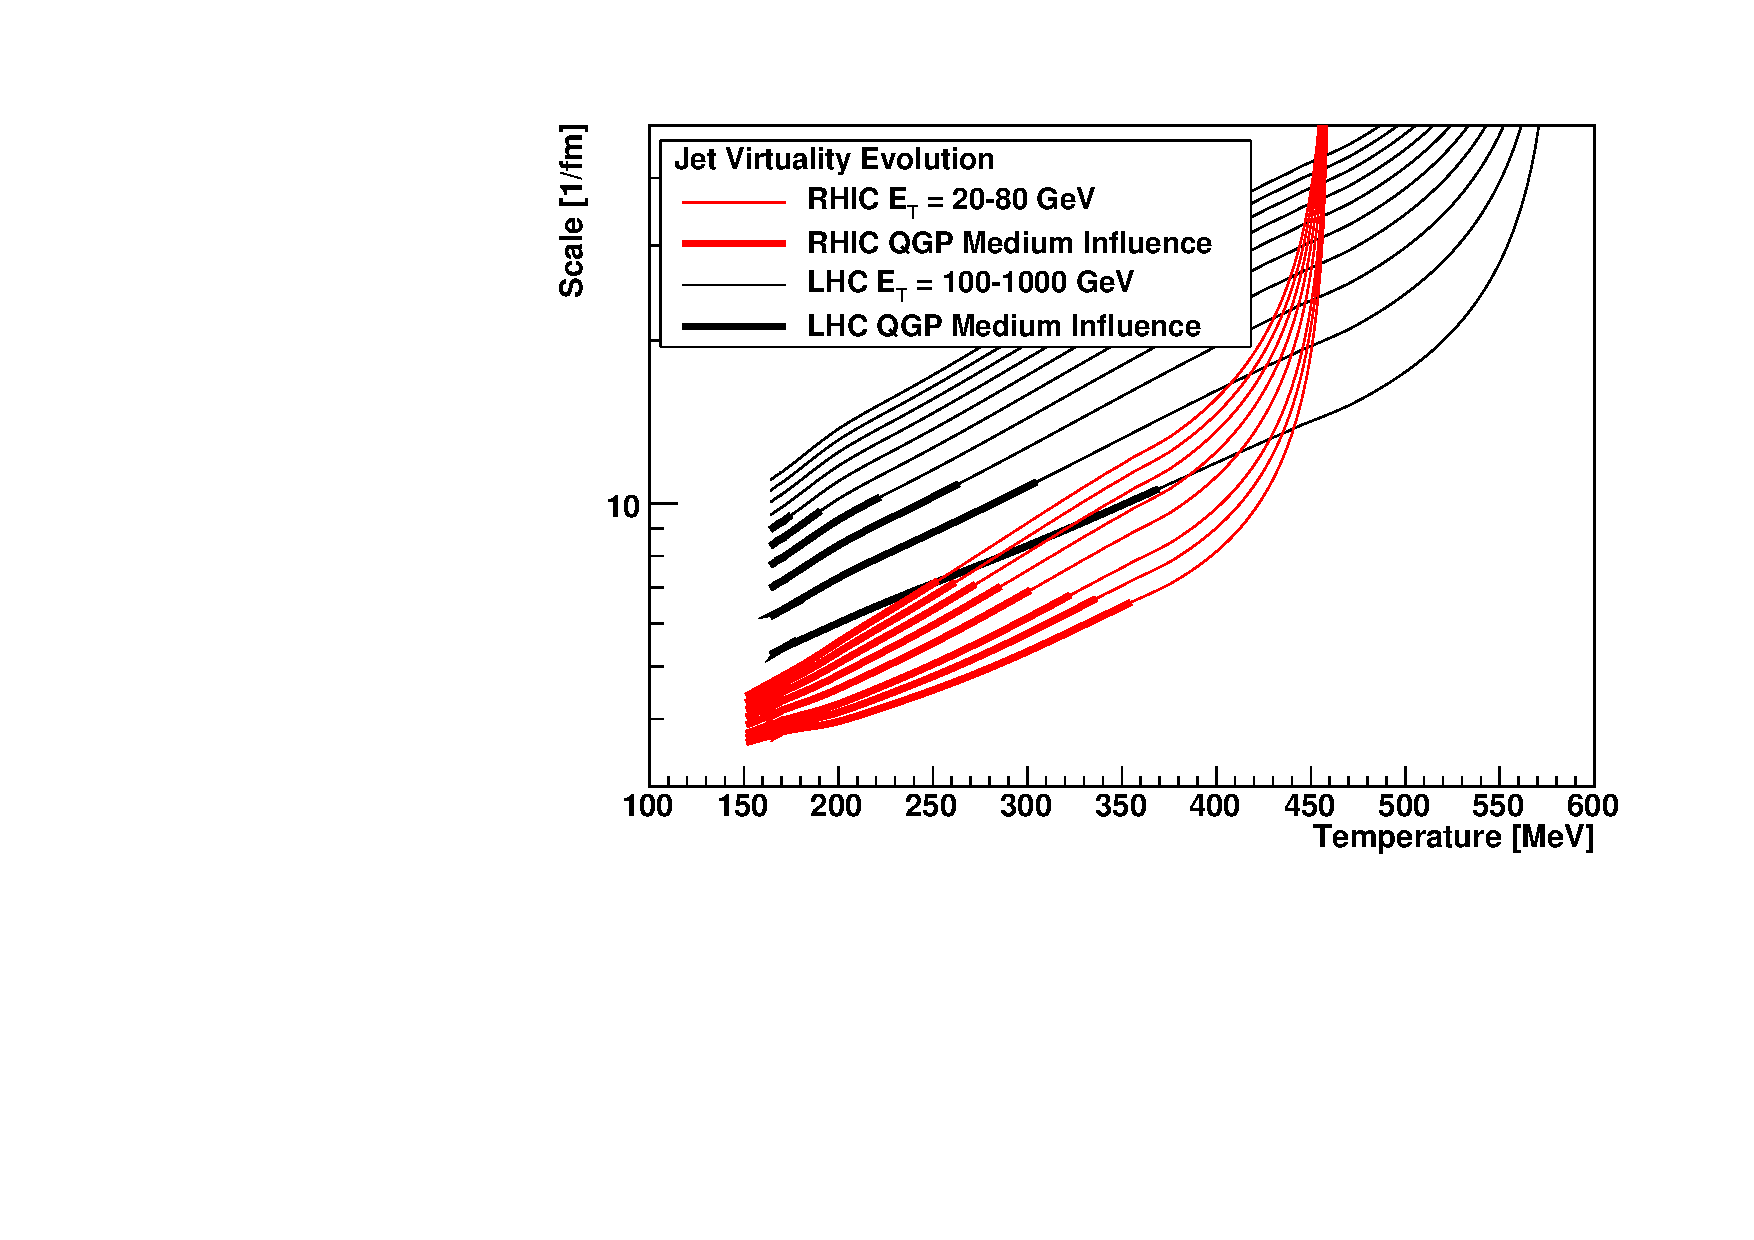
\includegraphics[width=0.95\linewidth]{figs/figure_nagle_jetvirtuality}
   \caption[Scale probed in the medium via high energy partons as a
   function of the local temperature in the medium]{Scale probed in
     the medium in [1/fm] via high energy partons as a function of the
     local temperature in the medium.  The red (black) curves are for
     different initial parton energies in the RHIC (LHC) medium.}
  \label{fig:magic2}
 \end{center}
\end{figure}

%\clearpage

\section{Current jet probe measurements}
 \label{currentjetdata}

CHECK THIS SUBSECTION IN THE ORIGINAL PROPOSAL - MAYBE NONE OF IT IS NEEDED HERE FOR THE PCDR (?)

 Jet quenching (i.e., the significant loss of energy for partons
 traversing the QGP) was discovered via measurements at RHIC of the
 suppression of single hadron yields compared to expectations from \pp
 collisions~\cite{Adcox:2001jp,Adler:2002xw}.  Since the time of that
 discovery there has been an enormous growth in jet quenching
 observables that have also pushed forward a next generation of
 analytic and Monte Carlo theoretical calculation to confront the
 data.

As detailed in Ref.~\cite{Adare:2008cg,Bass:2008rv}, many
formalisms assuming weakly coupled parton probes are able to achieve an equally
good description of the single inclusive hadron data at RHIC and the LHC.
The single high $p_T$ hadron suppression constrains
the $\hat{q}$ value within a model, but is not able to discriminate
between different energy loss mechanisms and formalisms for the
calculation.  Two-hadron correlations measure the correlated
fragmentation between hadrons from within the shower of one parton and
also between the hadrons from opposing scattered partons.  These
measurements, often quantified in terms of a nuclear modification
$I_{AA}$~\cite{Adare:2010ry,Adare:2010mq,Adams:2005ph}, are a
challenge for models to describe simultaneously~\cite{Nagle:2009wr}.

The total energy loss of the leading parton provides information on
one part of the parton-medium interaction.  Key information on the
nature of the particles in the medium being scattered from is
contained in how the soft (lower momentum) part of the parton shower
approaches equilibrium in the \qgp.  This information is 
accessible through full jet reconstruction, jet-hadron correlation,
and $\gamma$-jet correlation observables. 

The measurements of fully reconstructed jets and the particles correlated
with the jet (both inside the jet and outside) are crucial to testing
these pictures.  Not only does the strong coupling influence the
induced radiation from the hard parton (gluon bremsstrahlung)
and its inelastic collisions with the medium, but it also influences the way
soft partons are transported by the medium outside of the jet cone
as they fall into equilibrium with the medium.  Thus, the jet
observables combined with correlations get directly at the coupling of
the hard parton to the medium and the parton-parton coupling for the
medium partons themselves.

These jet observables are now available at the LHC.  The first results
based on reconstructed jets in heavy ion collisions were the
centrality dependent dijet asymmetries measured by
ATLAS~\cite{Aad:2010bu}. These results
%, shown in Figure~\ref{fig:atlasdijet}, 
indicate a substantial broadening of
dijet asymmetry $A_{J} = (E_{1}-E_{2})/(E_{1}+E_{2})$ distribution for
increasingly central \PbPb~collisions and the lack of modification to
the dijet azimuthal correlations.  The broadening of the $A_J$
distribution points to substantial energy loss for jets and the
unmodified azimuthal distribution shows that the opposing jet
$\Delta\phi$ distribution is not broadened as it traverses the matter.
%Figure~\ref{fig:cmsdijetsupp} shows CMS
%results~\cite{Chatrchyan:2011sx} quantifying the fraction of dijets
%which are balanced (with $A_J<0.15$) decreases with increasing
%centrality.

%\begin{figure}[t]
% \begin{center}
%    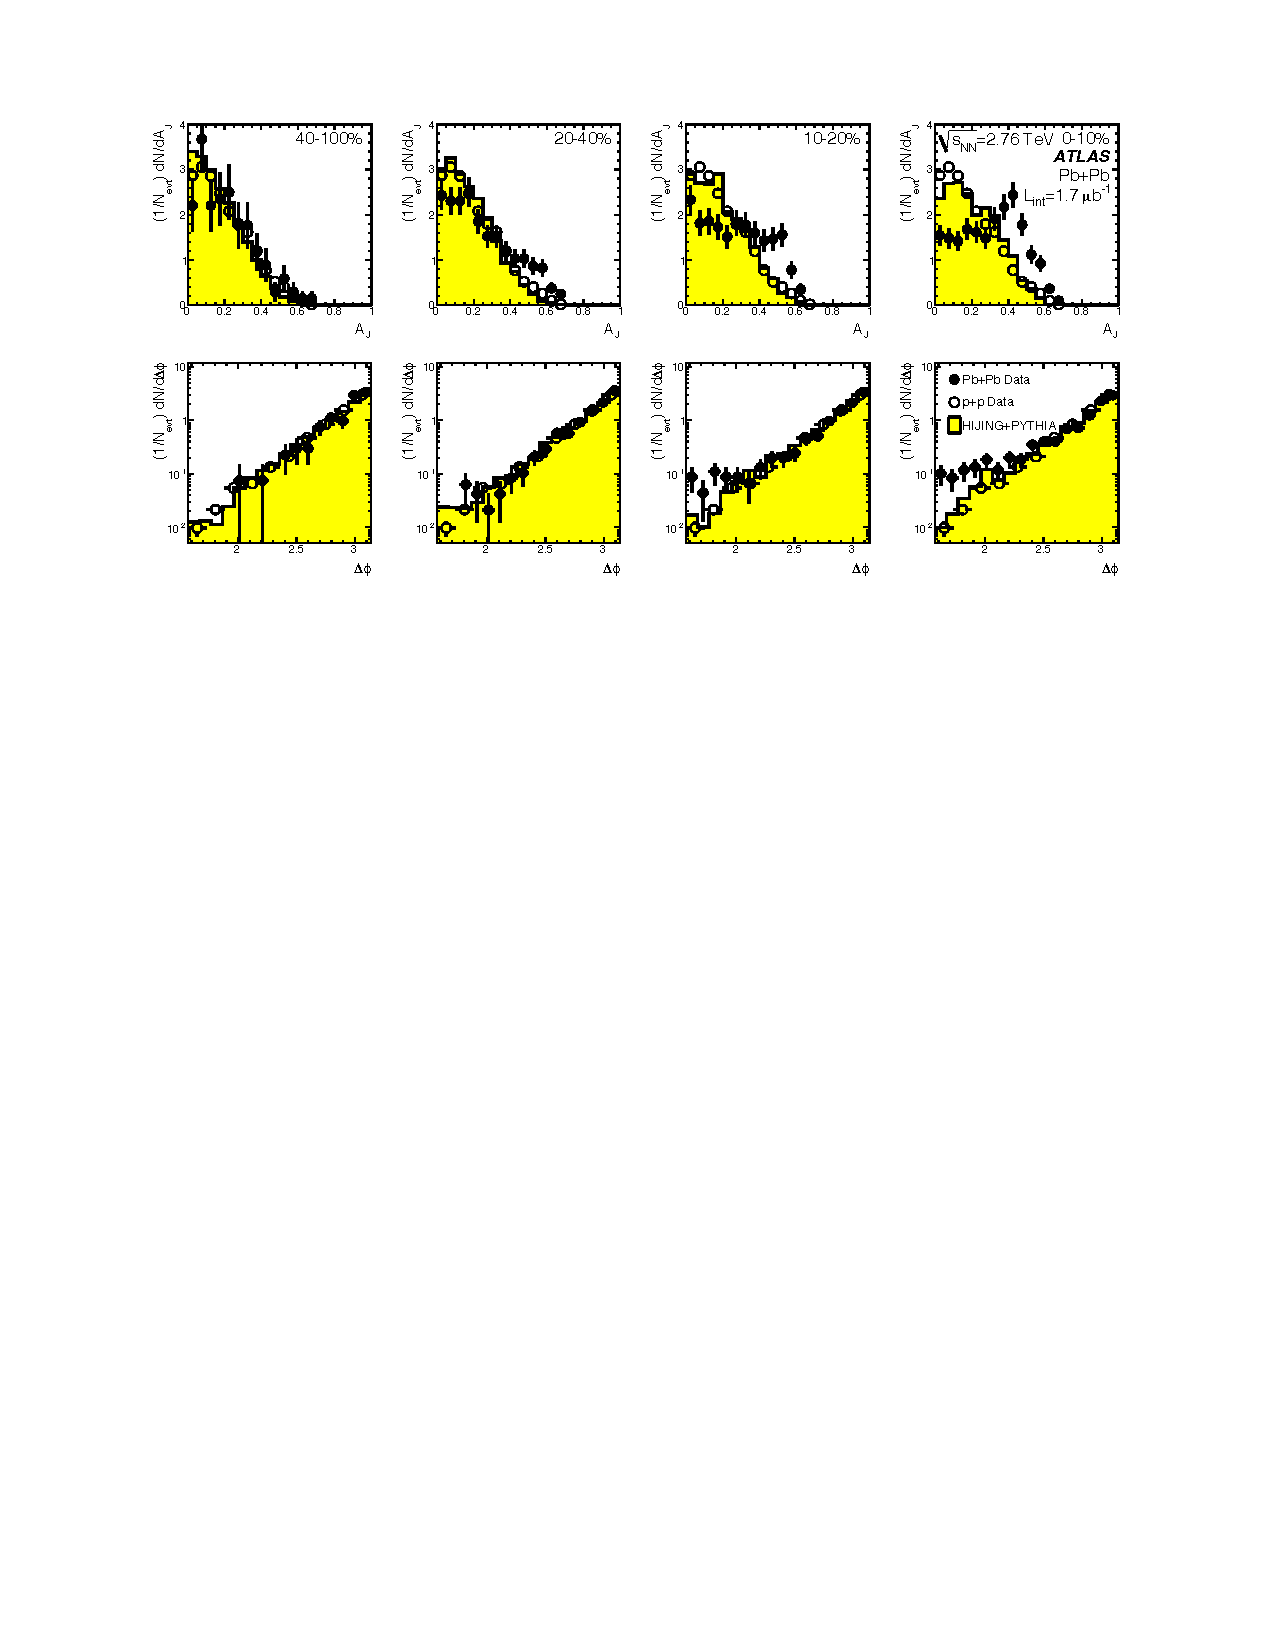
\includegraphics[trim = 2 2 2 2, clip, width=0.9\linewidth]{figs/figure_physicscase_atlasdijet}
 %   \caption[ATLAS $A_J$ and dijet $\Delta\phi$
 %   distributions]{\label{fig:atlasdijet}$A_J$ (top row) and dijet
 %     $\Delta\phi$ distribution from
 %     ATLAS~\protect\cite{Aad:2010bu}{}.  Jets are reconstructed with
 %     the anti-$k_T$ algorithm with $R=0.4$.  The leading jet has
 %     $E_T>100$~GeV and the associated jet has $E_T>25$~GeV.  \PbPb~
 %     data (solid points), \pp~data at 7~TeV (open points) and
 %     \pythia embedded in \hijing events and run through the ATLAS
 %     Monte Carlo (yellow histograms) are shown.  From
 %     Ref.~\protect\cite{Aad:2010bu}{}.}
 %\end{center}
%\end{figure}

%\begin{figure}[t]
% \begin{center}
%    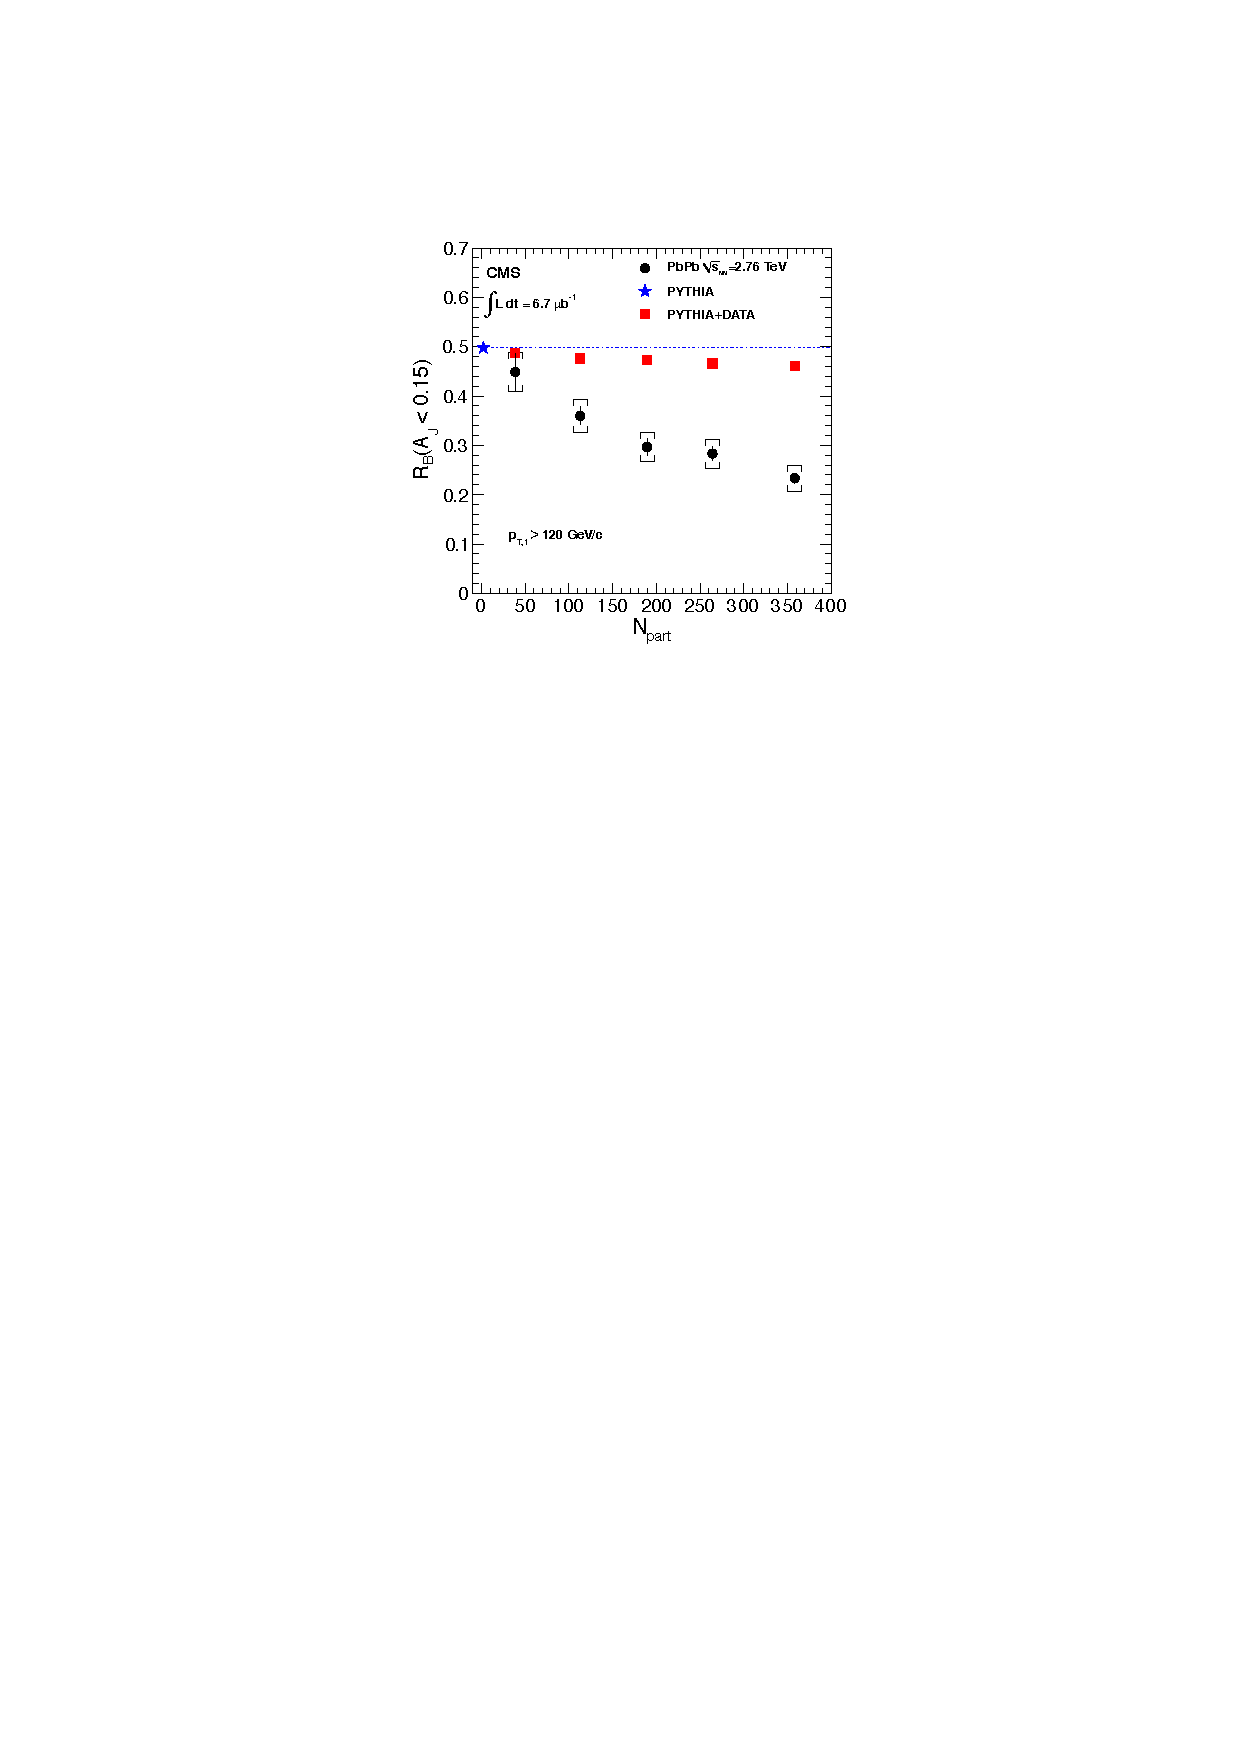
\includegraphics[trim = 2 2 2 2, clip, width=\onewidth]{figs/figure_physicscase_cmsdijet_supp}
%    \caption[Fraction of dijets with $A_J<0.15$ in \PbPb~collisions as
%    a function of centrality from CMS]{\label{fig:cmsdijetsupp}
%      Fraction of dijets which have $A_J<0.15$ in \PbPb~collisions as
%      a function of centrality.  Jets are reconstructed with an
%      iterative cone algorithm with a radius of 0.5.  The leading jet
%      is required to have an $E_T>120$~GeV and the associated jet has
%      $E_T>50$~GeV.  Results are shown for \PbPb~data (circles),
%      \pythia (star) and \pythia jets embedded into real data
%      (squares).  From Ref.~\protect\cite{Chatrchyan:2011sx}{}.}
% \end{center}
%\end{figure}

Direct photon-jet measurements are also a powerful tool to study jet
quenching. Unlike dijet measurements the photon passes through the
matter without losing energy, providing a cleaner handle on the
expected jet $p_T$~\cite{Wang:1996yh}.  CMS has results for
photons with $p_T>60$~GeV/c correlated with jets with
$p_T>30$~GeV/c~\cite{Chatrchyan:2012}.  Though with modest
statistical precision, the measurements indicate energy transported
outside the $R=0.3$ jet cone through medium interactions.  
Similar results from the ATLAS experiment 
again indicatE a shifting of energy outside the opposing jet radius.

Reconstructed jets have
significantly extended the kinematic range for jet quenching studies
at the LHC, and quenching effects are observed up to the highest
reconstructed jet energies ($>300$~GeV)~\cite{Chatrchyan:2012ni}.
They also provide constraints on the jet modification that are not
possible with particle based measurements.  For example, measurements from ATLAS
constrain jet fragmentation modification from vacuum fragmentation to
be small~\cite{Steinberg:2011qq} and  CMS results on jet-hadron
correlations have shown that the lost energy is recovered in low $p_T$
particles far from the jet cone~\cite{Chatrchyan:2011sx}.  
The lost energy is transported to very large angles
and the remaining jet fragments as it would in the vacuum.

Detector upgrades to PHENIX and STAR at RHIC with micro-vertex detectors will
allow the separate study of $c$ and $b$ quark probes of the medium, as tagged
via displaced vertex single electrons and reconstructed $D$ and $\Lambda_{c}$ hadrons.   Similar 
measurements at the LHC provide tagging of heavy flavor probes as well -- initial
results on beauty tagged jets from CMS are shown in the right panel of Figure~\ref{fig:gamma_bjet}.  
These measurements also provide insight on the different energy loss mechanisms,
in particular because initial measurements of non-photonic electrons from RHIC
challenge the radiative energy loss models.

%\begin{figure}[ht]
%  \centering
%  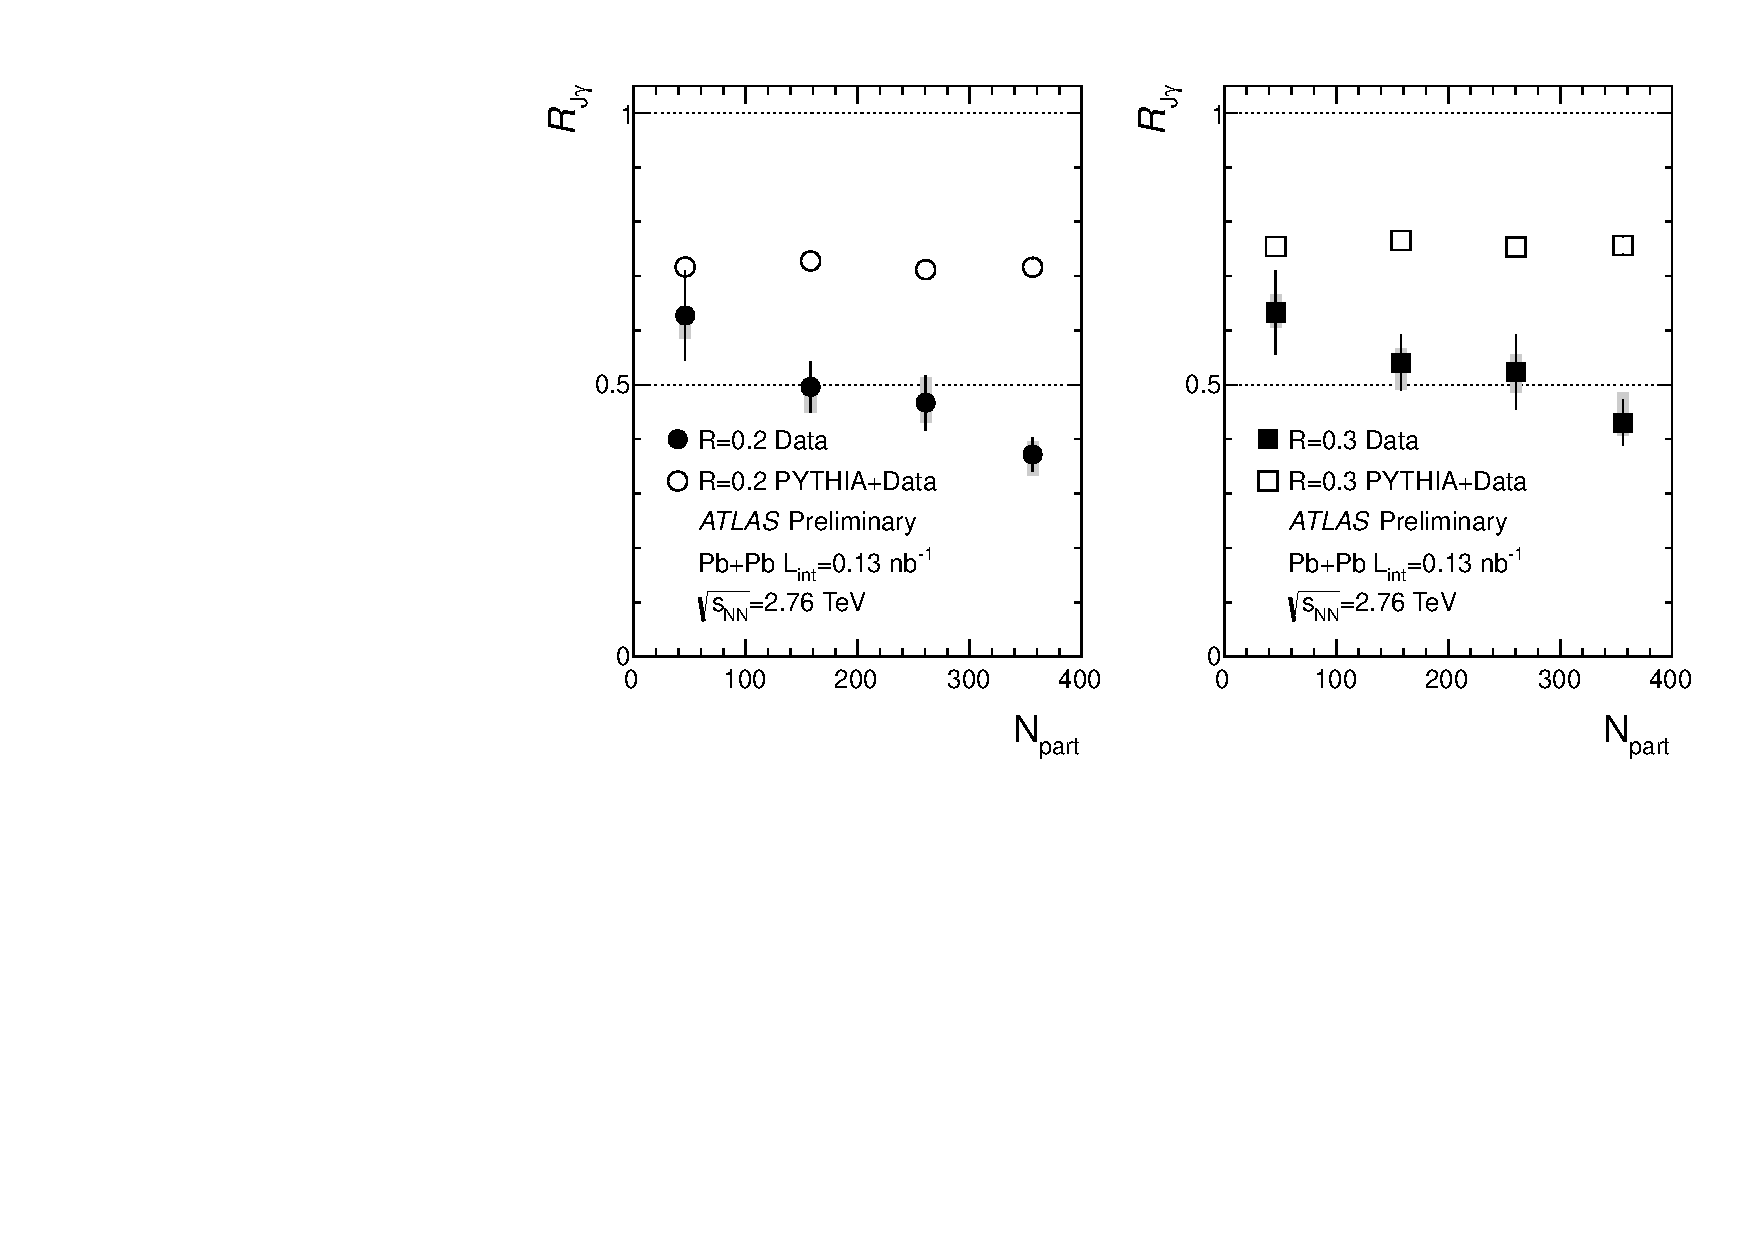
\includegraphics[width=0.50\linewidth]{figs/atlas_gammajet}
%  \hfill
%  \raisebox{0.12cm}{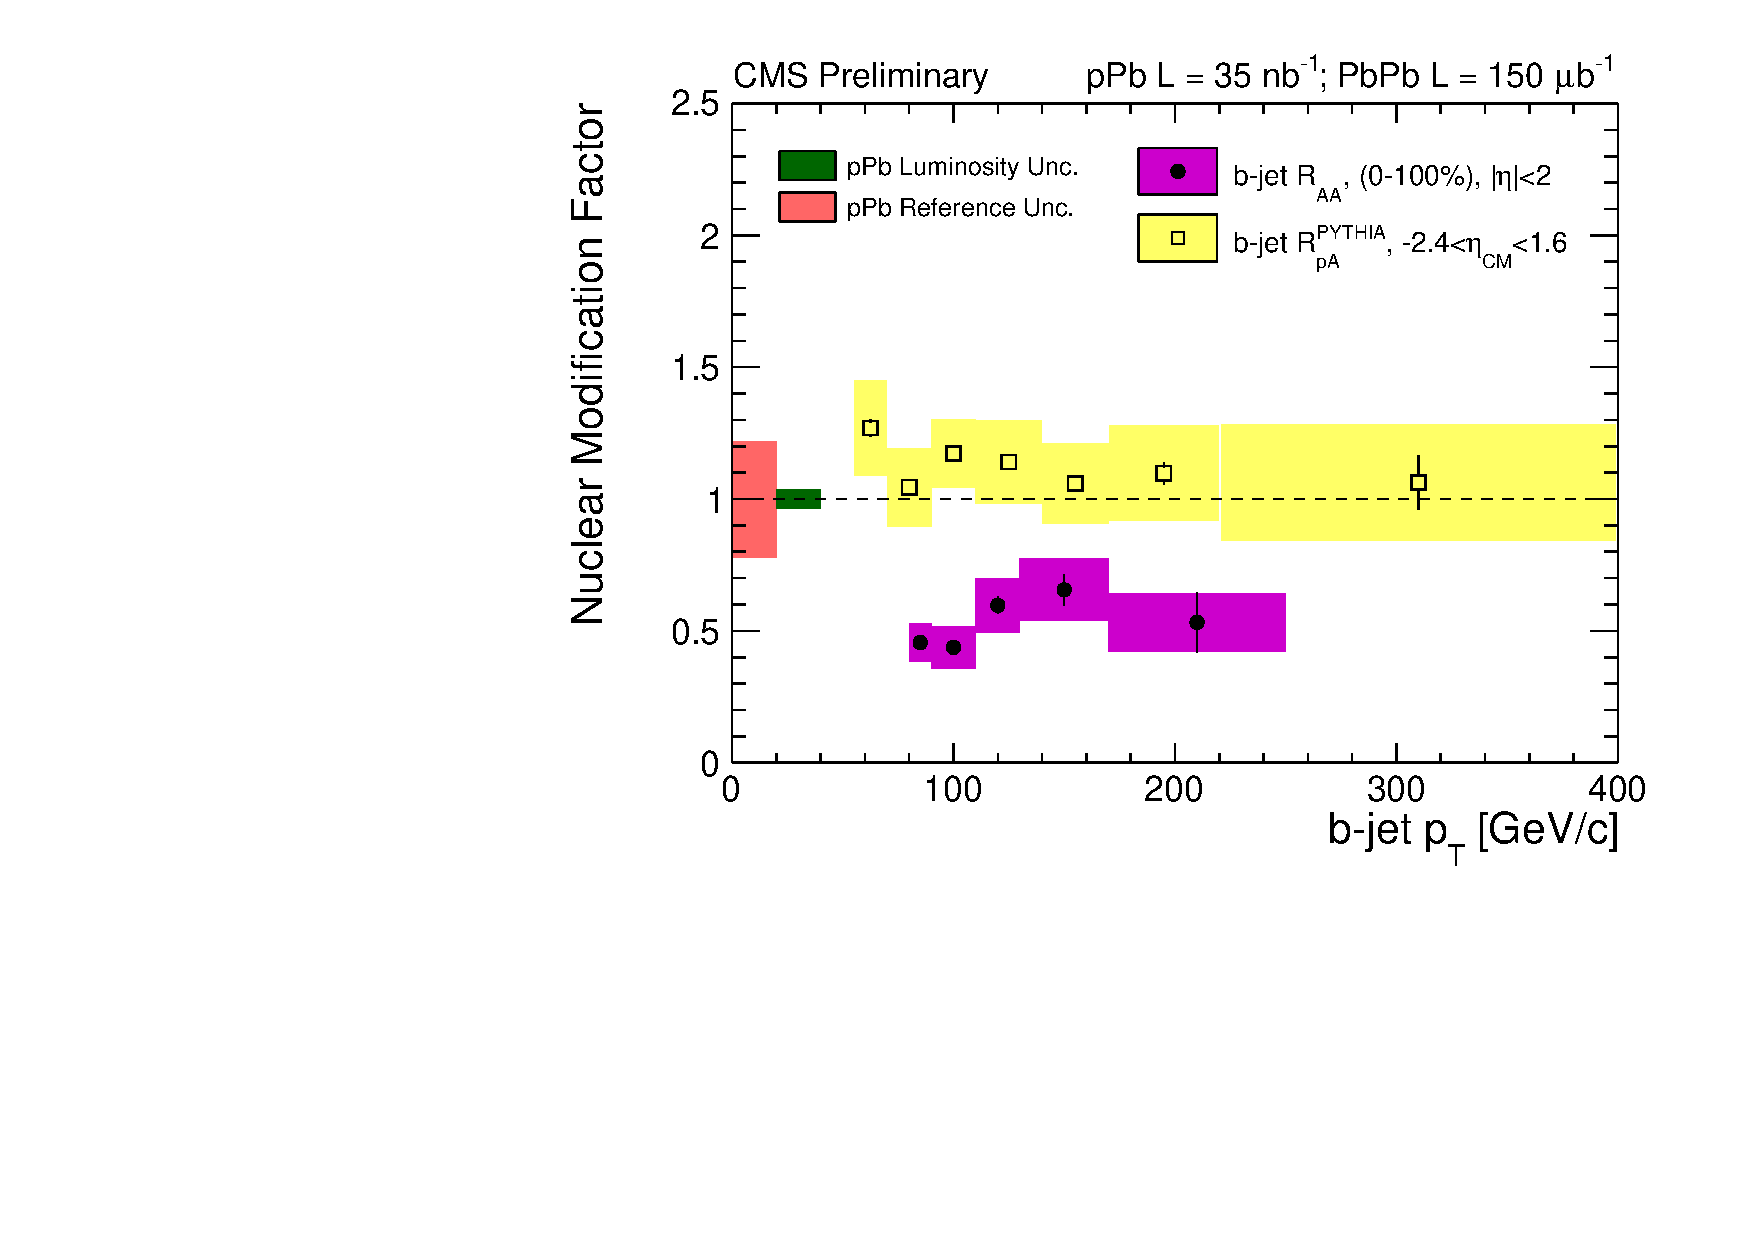
\includegraphics[width=0.43\linewidth]{figs/cms_bjet}}
%  \caption[ATLAS results on the change in balance of direct photons
%  and jets and CMS results on the \raa for beauty tagged jets in \pbpb
%  collisions at the LHC]{(left) ATLAS results on the change in balance
%    of direct photons and jets in \pbpb collisions at the LHC.
%    (right) CMS results on the \raa for beauty tagged jets in \pbpb
%    collisions at the LHC.  }
%  \label{fig:gamma_bjet}
%\end{figure}

There are other preliminary results on fully reconstructed jets from
both STAR~\cite{Caines:2011ew,Putschke:2011zz,Putschke:2008wn,Jacobs:2010wq}
and PHENIX experiments~\cite{Lai:2011zzb,Lai:2009zq}.  However, these
results have not yet proceeded to publication in part due to limitations
in the measurement capabilities.  In this proposal we demonstrate that
a comprehensive jet detector (sPHENIX) with large, uniform acceptance
and high rate capability, combined with the now completed RHIC
luminosity upgrade can perform these measurements to access this key
physics.

%Figure~\ref{fig:star_hjet}
%shows results from the STAR collaboration~\cite{Adamczyk:2013jei} on
%correlations between reconstructed trigger jets and single charged
%hadrons. The experimental results show the difference in the away-side
%momentum of hadrons between Au$+$Au and \pp events.  The extent to
%which this value differs from zero is an indication of the strength of
%the medium modification of the fragmentation process.  The figure also
%compares these results to calculations obtained using the YAJEM-DE
%model that qualitatively reproduces the data.

%\begin{figure}[ht]
%  \centering
%  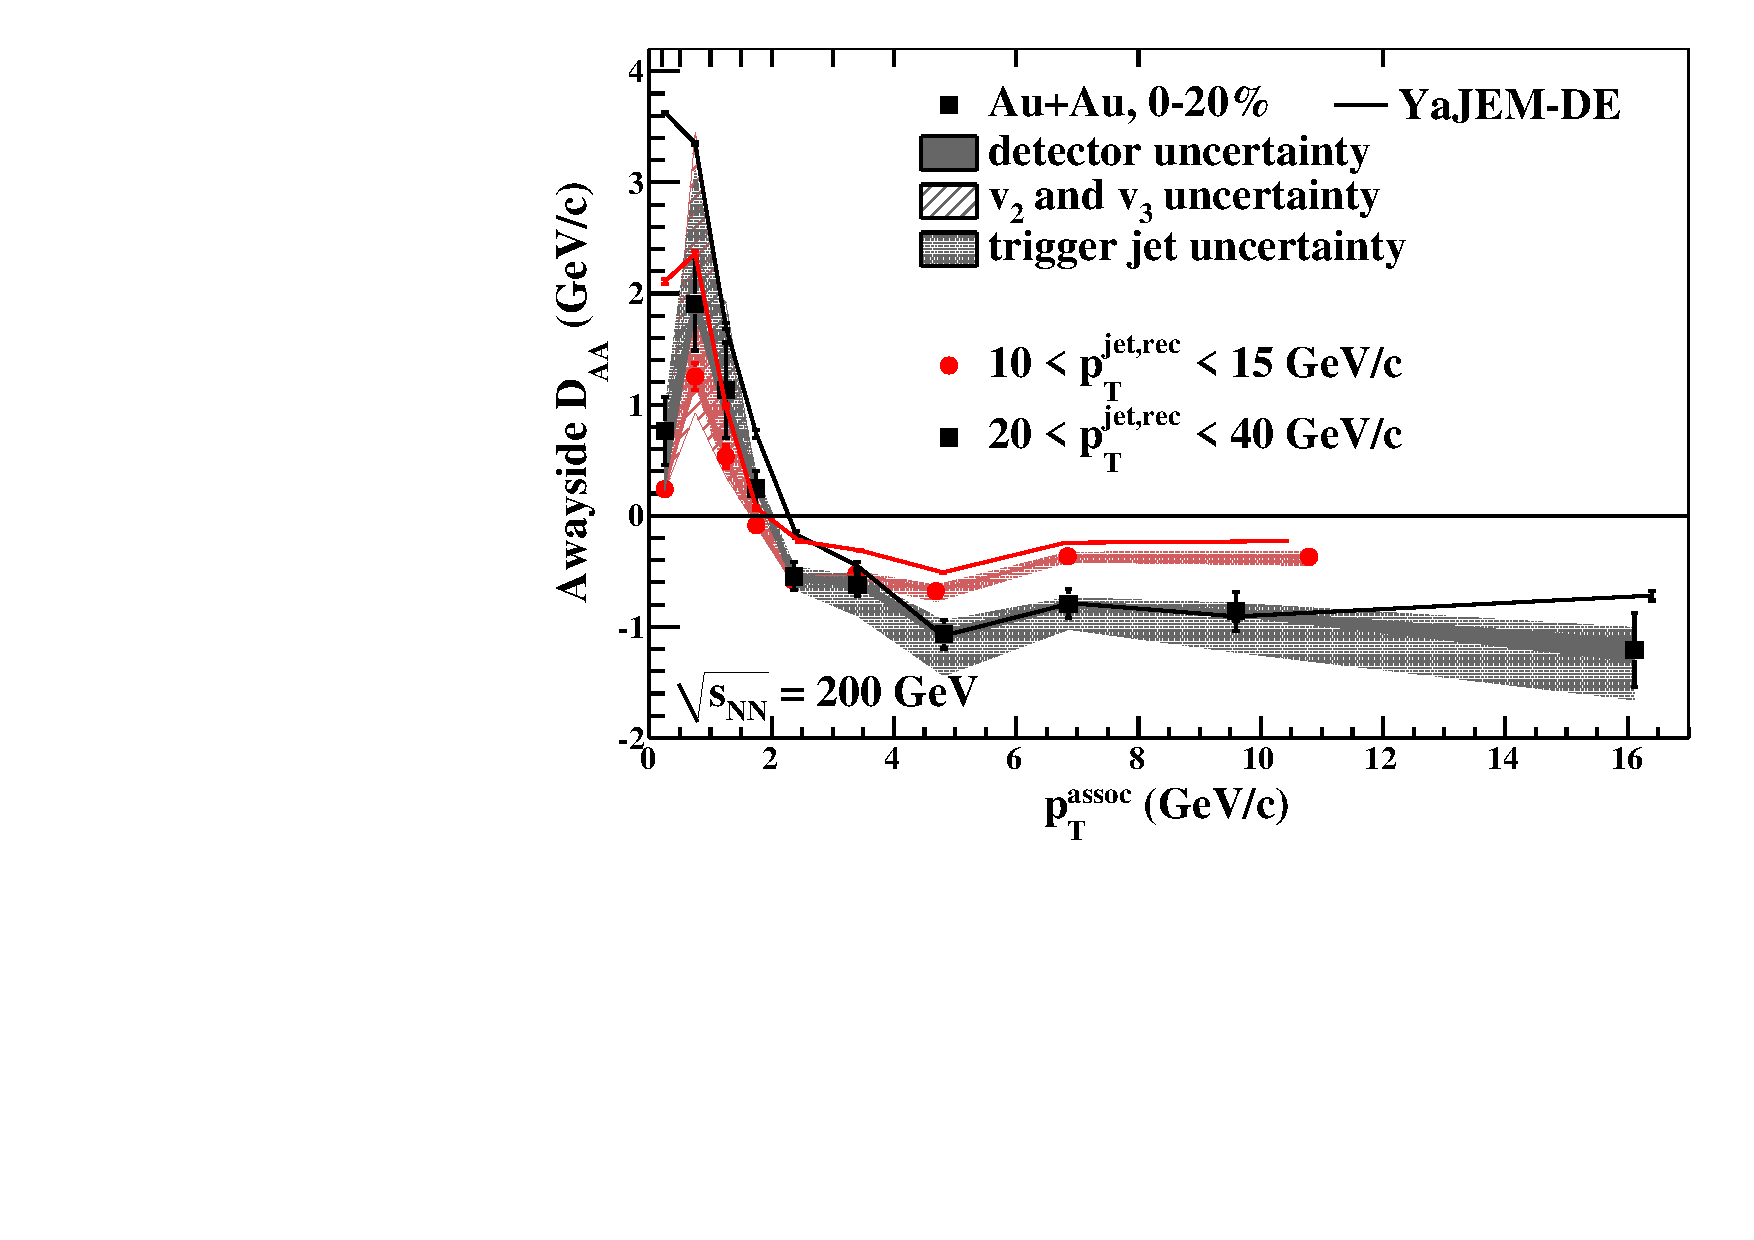
\includegraphics[width=0.7\linewidth]{figs/star_hjet_fig4}
%  \caption[The away-side momentum difference, $D_{AA}$, of hadrons
%  between \auau and \pp events, as measured by STAR]{The away-side
%    momentum difference, $D_{AA}$, of hadrons between \auau and \pp
%    events, as measured by STAR~\cite{Adamczyk:2013jei}, showing
%    medium modification of jet fragmentation.}
%  \label{fig:star_hjet}
%\end{figure}

%Figure~\ref{fig:guntheruber} shows a compilation panel with results
%from RHIC preliminary jet results and LHC jet results.  They indicate
%that with this set of observables, the behavior is quite different at
%RHIC and the LHC.  Whether the significant radius $R$ dependence of
%jet suppression \raa at RHIC, not observed at the LHC, is the result
%of engineered bias selections on the STAR results remains to be
%tested.  In addition, the recovery of most energy within $R=0.4$ is an
%exciting result from STAR which could potentially indicate a different
%redistribution of energy in the RHIC created \qgp.

%\begin{figure}[t]
% \begin{center}
%   \fbox{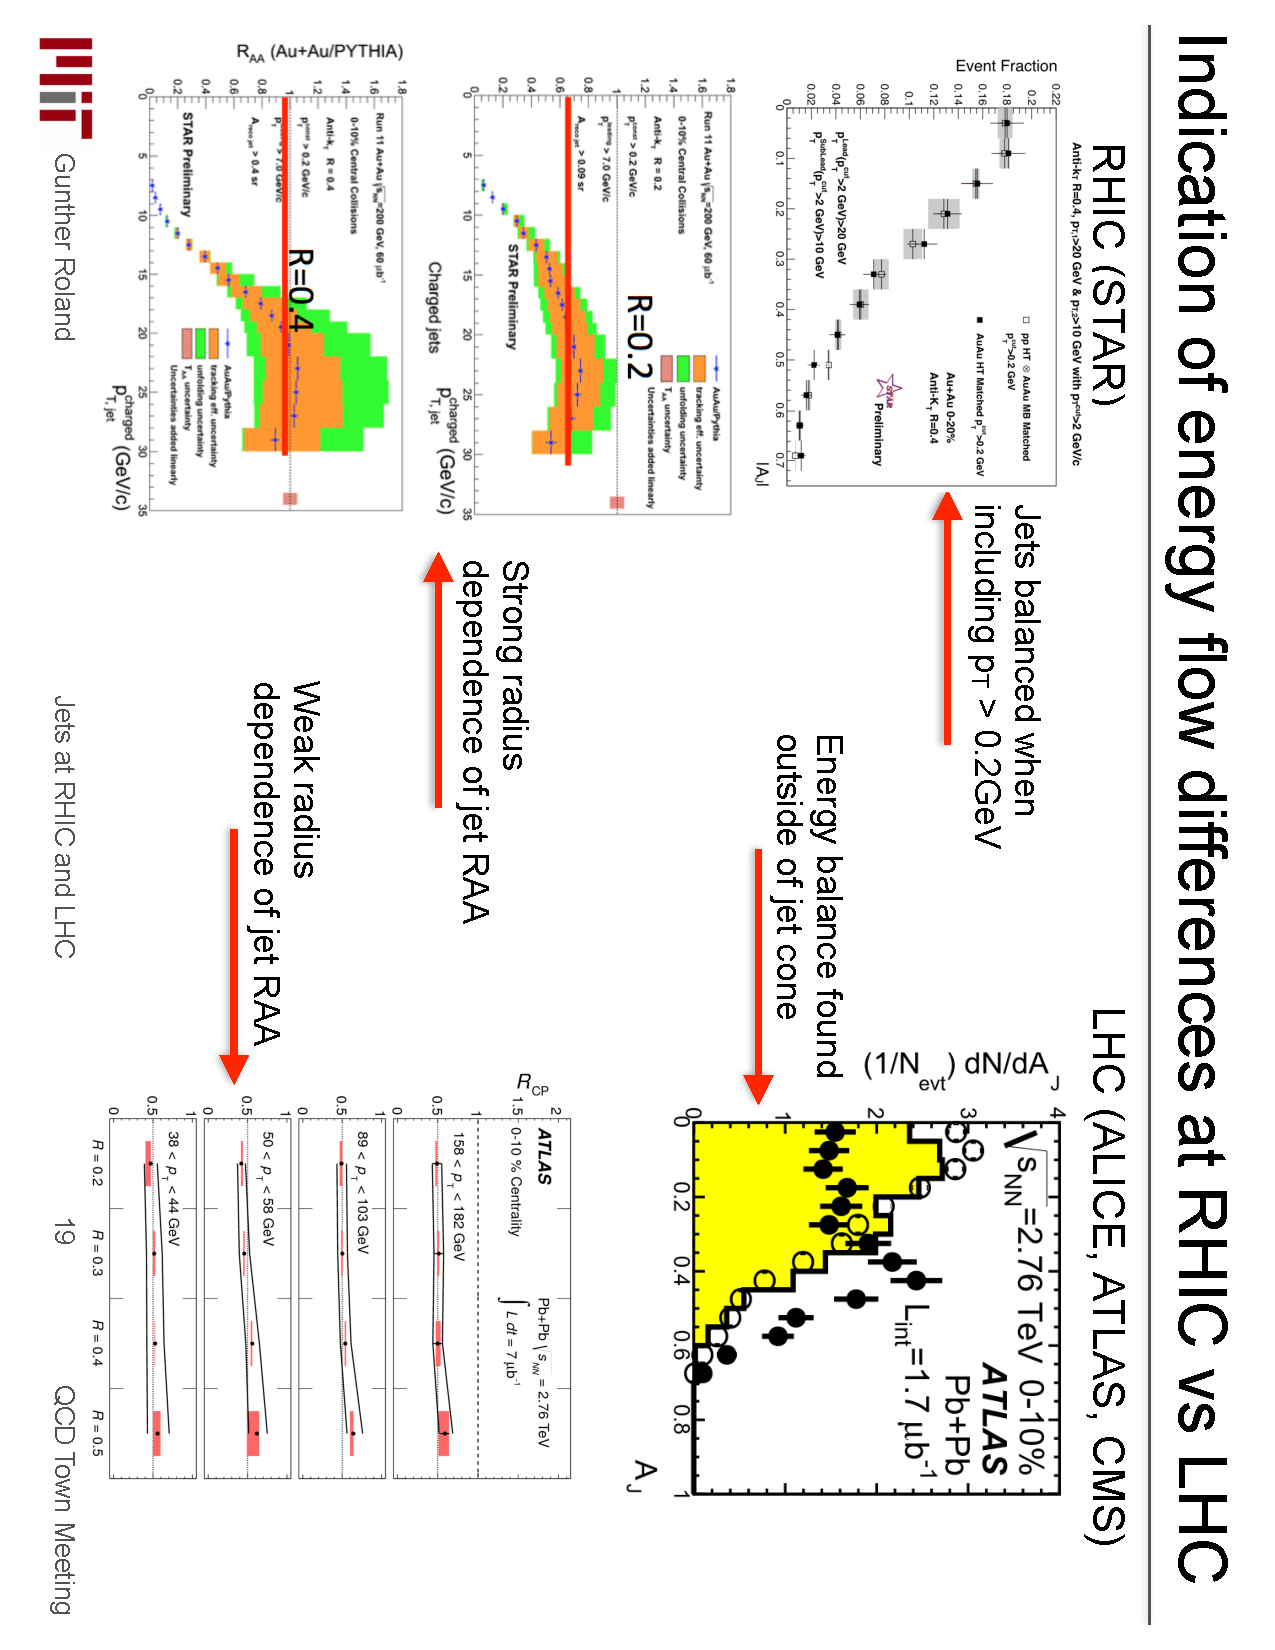
\includegraphics[angle=90,width=\linewidth]{figs/figure_gunther_compare_rhiclhc}}
%   \caption[Slide from G. Roland's talk at the QCD Town Meeting
%   (September 2014) contrasting preliminary RHIC results from STAR for
%   jet \raa and dijet asymmetry $A_J$  with LHC results]{ Slide from G. %Roland's talk at the QCD Town Meeting
%     (September 2014).  Shown are preliminary RHIC results from STAR
%     for jet \raa and dijet asymmetry $A_J$ in comparison with LHC
%     results.  The initial observation is for quite different trends.
%     Data with overlapping energy ranges and comparable jet algorithms
%     and jet bias selections from sPHENIX will shed significant light
%     on the underlying physics differences.
%    \label{fig:guntheruber}
%  }
% \end{center}
%\end{figure}

It is clear that in addition to extending the RHIC observables to
include fully reconstructed jets and $\gamma$-jet correlations,
theoretical development work is required for converging to a coherent
'standard model' of the medium coupling strength and the nature of the
probe-medium interaction.  In the next section, we detail positive
steps in this direction.

%\clearpage

\section{Theoretical calculations of jets at RHIC}
\label{sec:jetcalculations}

Motivated in part by the new information provided by LHC jet results
and the comparison of RHIC and LHC single and di-hadron results, the
theoretical community is actively working to understand the detailed
probe-medium interactions.  The challenge is to understand not only
the energy loss of the leading parton, but how the parton shower
evolves in medium and how much of the lost energy is re-distributed in
the \qgp.  Theoretical calculations attempting to describe the wealth
of new data from RHIC and the LHC have not yet reconciled some of the
basic features, with some models including large energy transfer to
the medium as heat (for example~\cite{CasalderreySolana:2011rq}) and
others with mostly radiative energy loss (for
example~\cite{Renk:2012cb,Renk:2011wb}).  None of the current
calculations available has been confronted with the full set of jet
probe observables from RHIC and the LHC.  Measurements of jets at RHIC
energies and with jets over a different kinematic range allow for
specific tests of these varying pictures.  In this section, we give a
brief review of a subset of calculations for jet observables at RHIC
enabled by the sPHENIX upgrade and highlight the sensitivity of these
observables to the underlying physics.

Much of this work has been carried out under the auspices of the
Department of Energy Topical Collaboration on Jet and Electromagnetic
Tomography of Extreme Phases of Matter in Heavy-ion Collisions
~\cite{jetcollaboration}.  Workshops held by the JET Collaboration at
Duke University in March 2012 and Wayne State University in August
2013 and 2014 have been dedicated to the topic of jet measurements at RHIC.
These workshops were attended by theorists as well as experimentalists
from both RHIC and the LHC.  This is an active collaborative effort.

In order to overcome specific theoretical hurdles regarding analytic
parton energy loss calculations and to couple these calculations with
realistic models of the QGP space-time evolution, Monte Carlo
approaches have been developed (as
examples~\cite{Zapp:2009pu,Renk:2010zx,Young:2011va,ColemanSmith:2011wd,Lokhtin:2011qq,Armesto:2009zc}).
Here we describe RHIC energy jet probe results from specific theory
groups utilizing different techniques for calculating the jet-medium
interactions.  These efforts indicate a strong theoretical interest
and the potential constraining power of a comprehensive jet physics
program at RHIC.

Jets provide a very rich spectrum of physics observables, ranging from
single jet observables such as \raa, to correlations of jets with
single particles, to correlations of trigger jets with other jets in
the event.  An example of how one can exploit this variety can be
found in recent calculations by Renk~\cite{Renk:2012ve}.
%Figure~\ref{fig:renk_jet_engineering} is based on calculations using
%the YaJEM model to illustrate what could be called ``jet surface
%engineering''.  
Triggers ranging from single hadrons on up to ideally
reconstructed jets are used to form correlations with another jet in
the event.  The different triggers demonstrate different degrees of
surface bias in the production point of the ``dijet'' and this bias
itself can be used as a lever to investigate properties of the medium.

%\begin{figure}[ht]
%  \centering
%  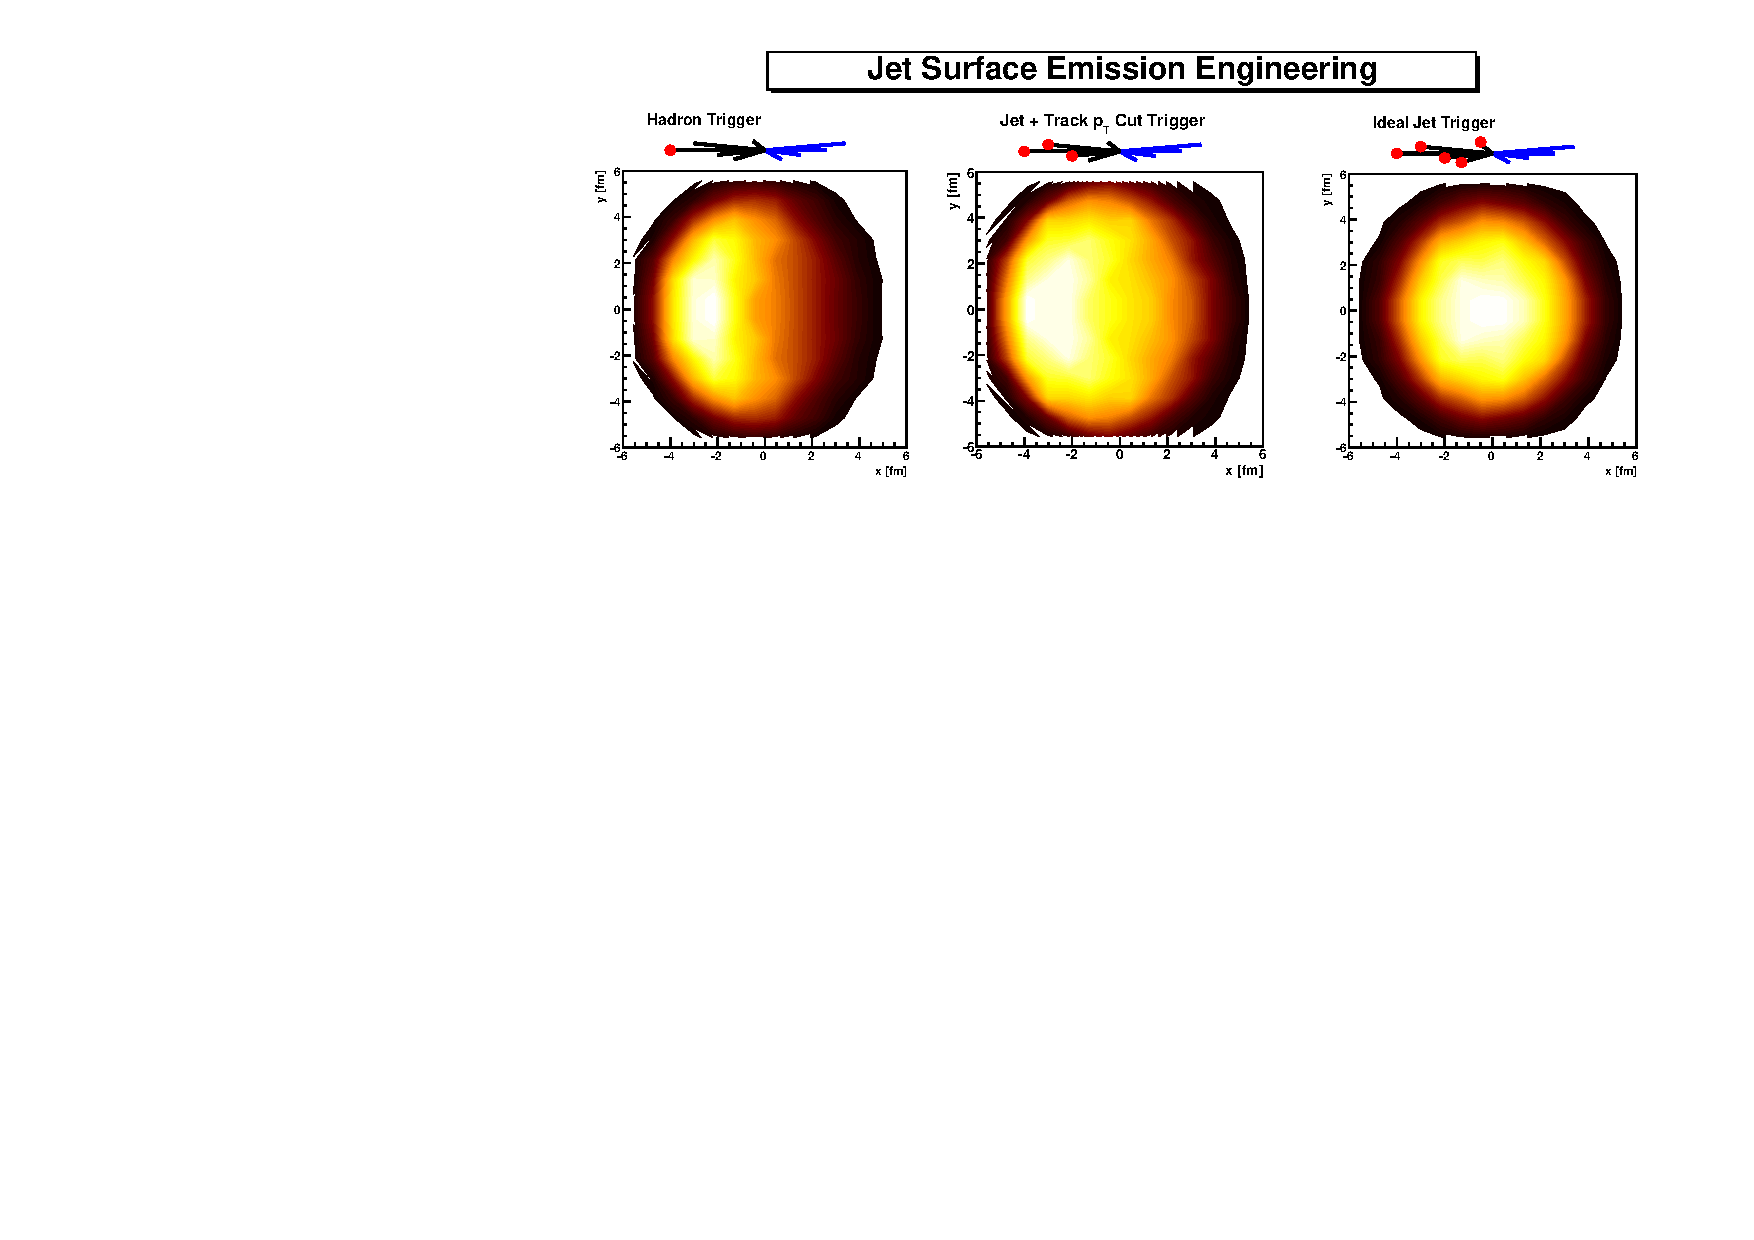
\includegraphics[trim = 30 0 30 30, clip, width=\linewidth]{figs/figure_jetsurfaceengineering}
%  \caption[Dijet surface bias in YaJEM for various trigger
%  definitions]{Dijet surface bias in YaJEM for various trigger
%    definitions. As the trigger is changed from a single hadron (left)
%    to a reconstructed jet with a minimum $p_T$ selection on charged
%    tracks and electromagnetic clusters (middle) to an ideally
%    reconstructed jet (right), the surface bias in the production
%    point becomes less pronounced. sPHENIX is capable of all three
%    types of measurements.  (Based on figure taken
%    from~\cite{Renk:2012ve}.)}
%  \label{fig:renk_jet_engineering}
%\end{figure}

\begin{figure}[ht]
 \begin{center}
    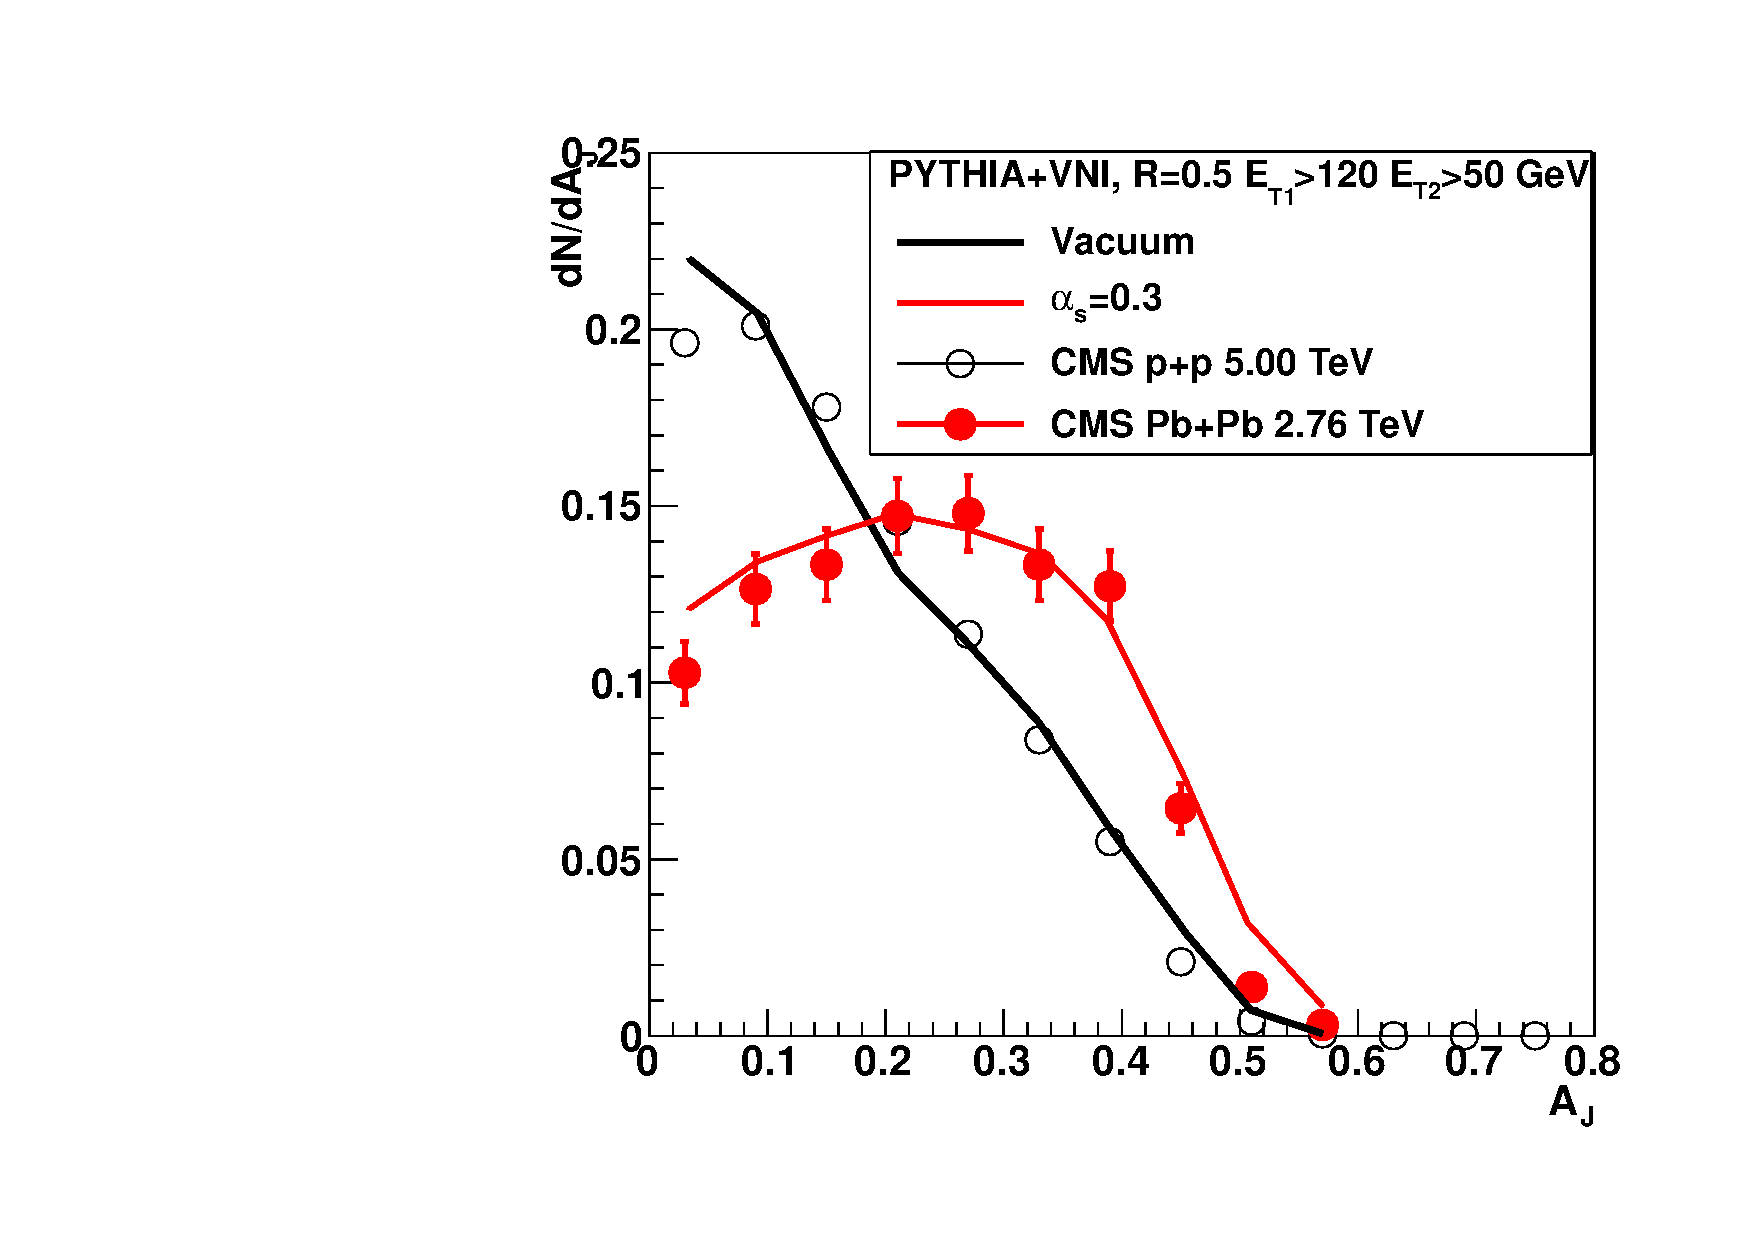
\includegraphics[trim = 2 2 2 2, clip, width=\twowidth]{figs/figure_physicscase_colemansmith_lhc_aj}
    \hfill
    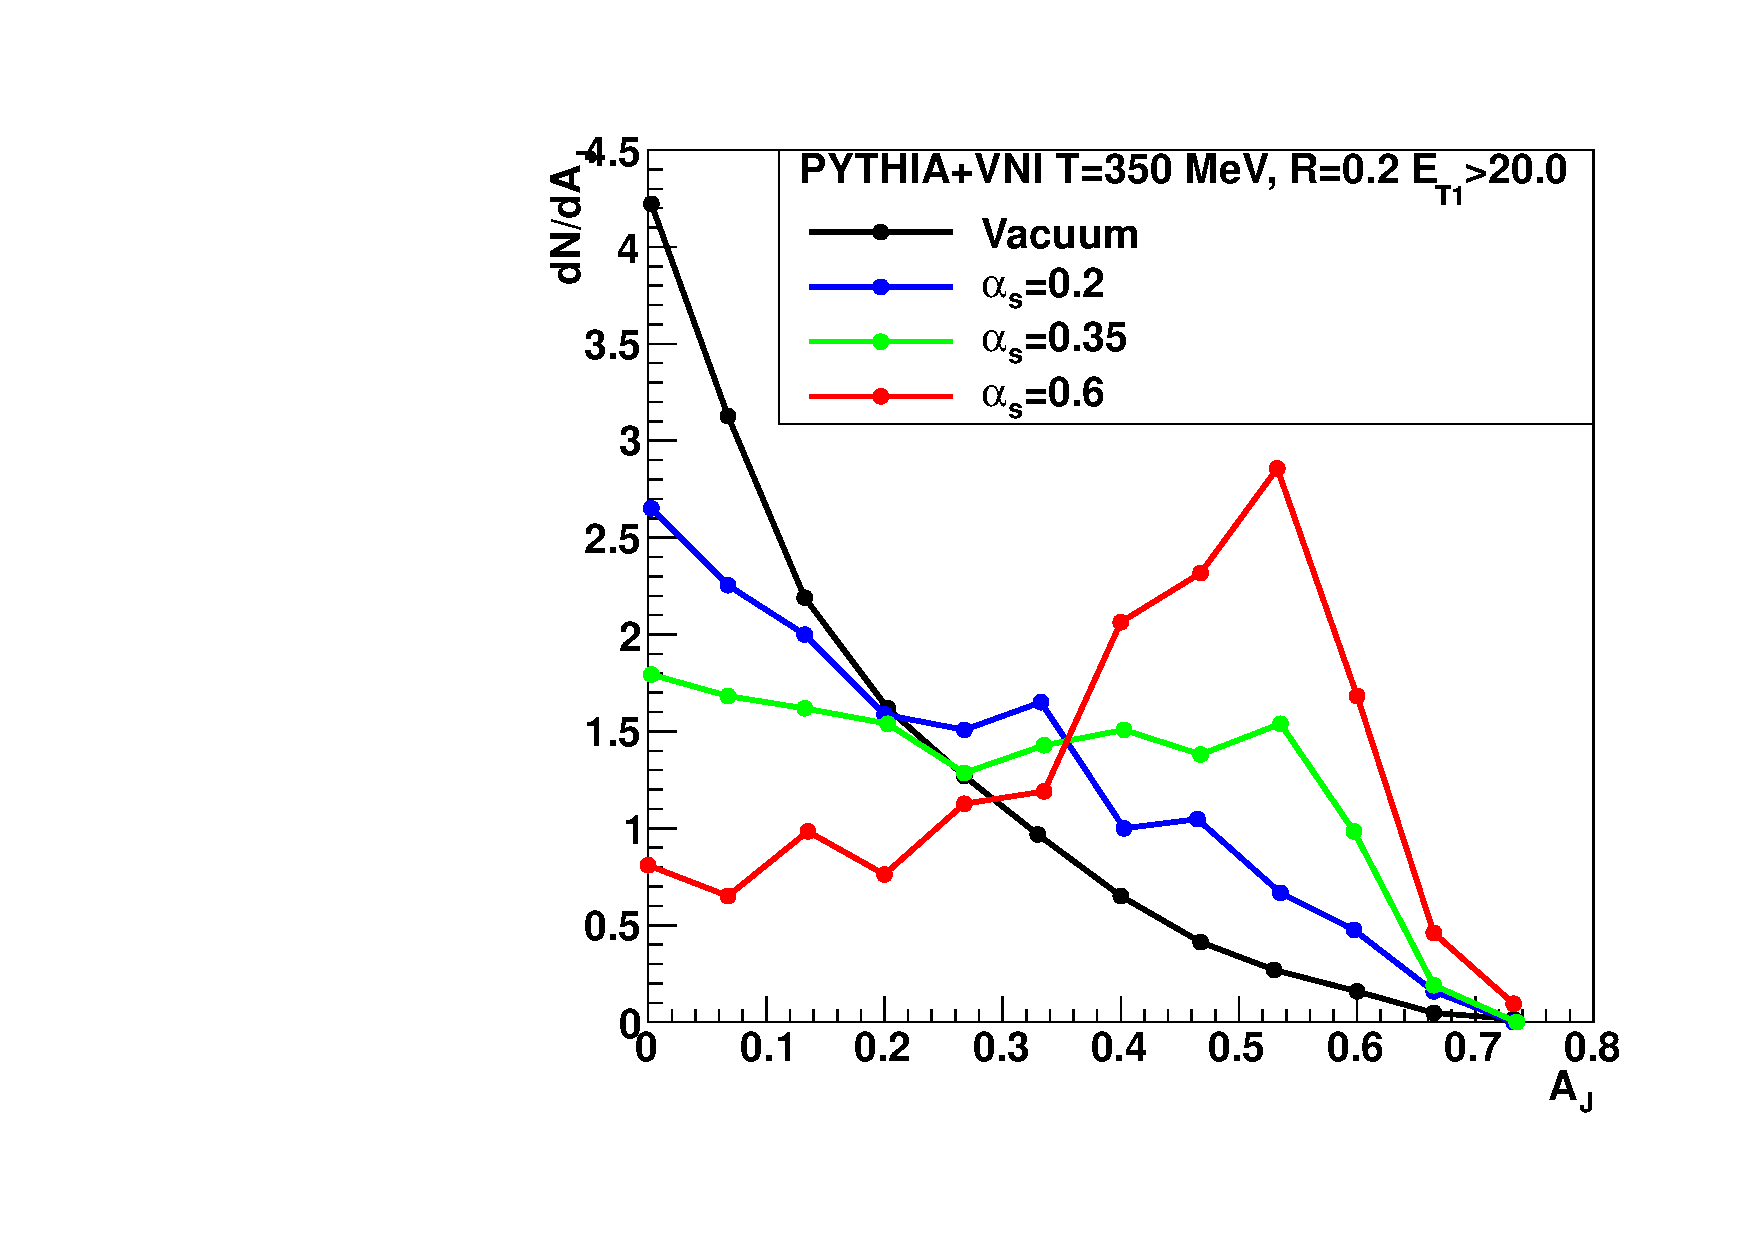
\includegraphics[trim = 2 2 2 2, clip,width=\twowidth]{figs/figure_physicscase_colemansmith_rhic_aj_alphasensitivity}
    \caption[Dijet $A_J$ in VNI parton cascade compared to the CMS
    data and calculation for RHIC energies of $A_J$ for different
    values of $\alpha_s$]{\label{fig:colemansmith1}(left) Calculation
      in VNI parton cascade of dijet $A_J$ with $T=0.35$~GeV and
      $\alpha_s=0.3$ compared to the CMS
      data~\protect\cite{ColemanSmith:2011rw}{}.  (right) Calculation
      for RHIC jet energies, $E_{T,1}>20$~GeV, for a circular
      geometry of radius 5\,fm of $A_J$ for different values of
      $\alpha_s$ increasing to $\alpha_s=0.6$ (red
      line)~\protect\cite{ColemanSmith:2012vr}{}.}
 \end{center}
\end{figure}

We show results are from Coleman-Smith and
collaborators~\cite{ColemanSmith:2011rw,ColemanSmith:2011wd} where
they extract jet parton showers from \pythia (turning off
hadronization) and then embed the partons into a deconfined \qgp,
modeled with the VNI parton cascade~\cite{Geiger:1991nj}.  For the
calculations shown here, the background medium consists of a cylinder
of deconfined quarks and gluons at a uniform temperature.  One
excellent feature of the calculation is that it provides the ability
to track each individual parton and thus not only look at the full
time evolution of scattered partons from the shower, but also medium
partons that are kicked up and can contribute particles to the
reconstructed jets.

Calculation results for the dijet asymmetry $A_{J} =
(E_{1}-E_{2})/(E_{1}+E_{2})$ in a QGP with a temperature appropriate
for LHC collisions and fixed $\alpha_{s}=0.3$ are shown in
Figure~\ref{fig:colemansmith1} (left
panel)~\cite{ColemanSmith:2011rw}.  The jets in the calculation are
reconstructed with the anti-$k_T$ algorithm with radius parameter $R =
0.5$ and then smeared by a simulated jet resolution of
100\%/$\sqrt{E}$, and with requirements of $E_{T1}>120$~GeV and
$E_{T2}>50$~GeV on the leading and sub-leading jet, respectively.
The calculated $A_J$ distributions reproduce the CMS experimental
data~\cite{Chatrchyan:2011sx}.

In Figure~\ref{fig:colemansmith1} (right panel) the calculation is
repeated with a medium temperature appropriate for RHIC collisions and
with RHIC observable jet energies, $E_{T1} > 20$~GeV and $R = 0.2$.
The calculation is carried out for different coupling strengths
$\alpha_{s}$ between partons in the medium themselves and the parton
probe and medium partons.  The variation in the value of $\alpha_{s}$
should be viewed as changing the effective coupling in the many-body
environment of the QGP.  It is interesting to note that in the parton
cascade BAMPS, the authors find a coupling of $\alpha_{s} \approx 0.6$
is required to describe the bulk medium flow~\cite{Wesp:2011yy}.
These results indicate sizable modification to the dijet asymmetry and
thus excellent sensitivity to the effective coupling to the medium at
RHIC energies.  

%\begin{figure}[!hbt]
%  \centering
%    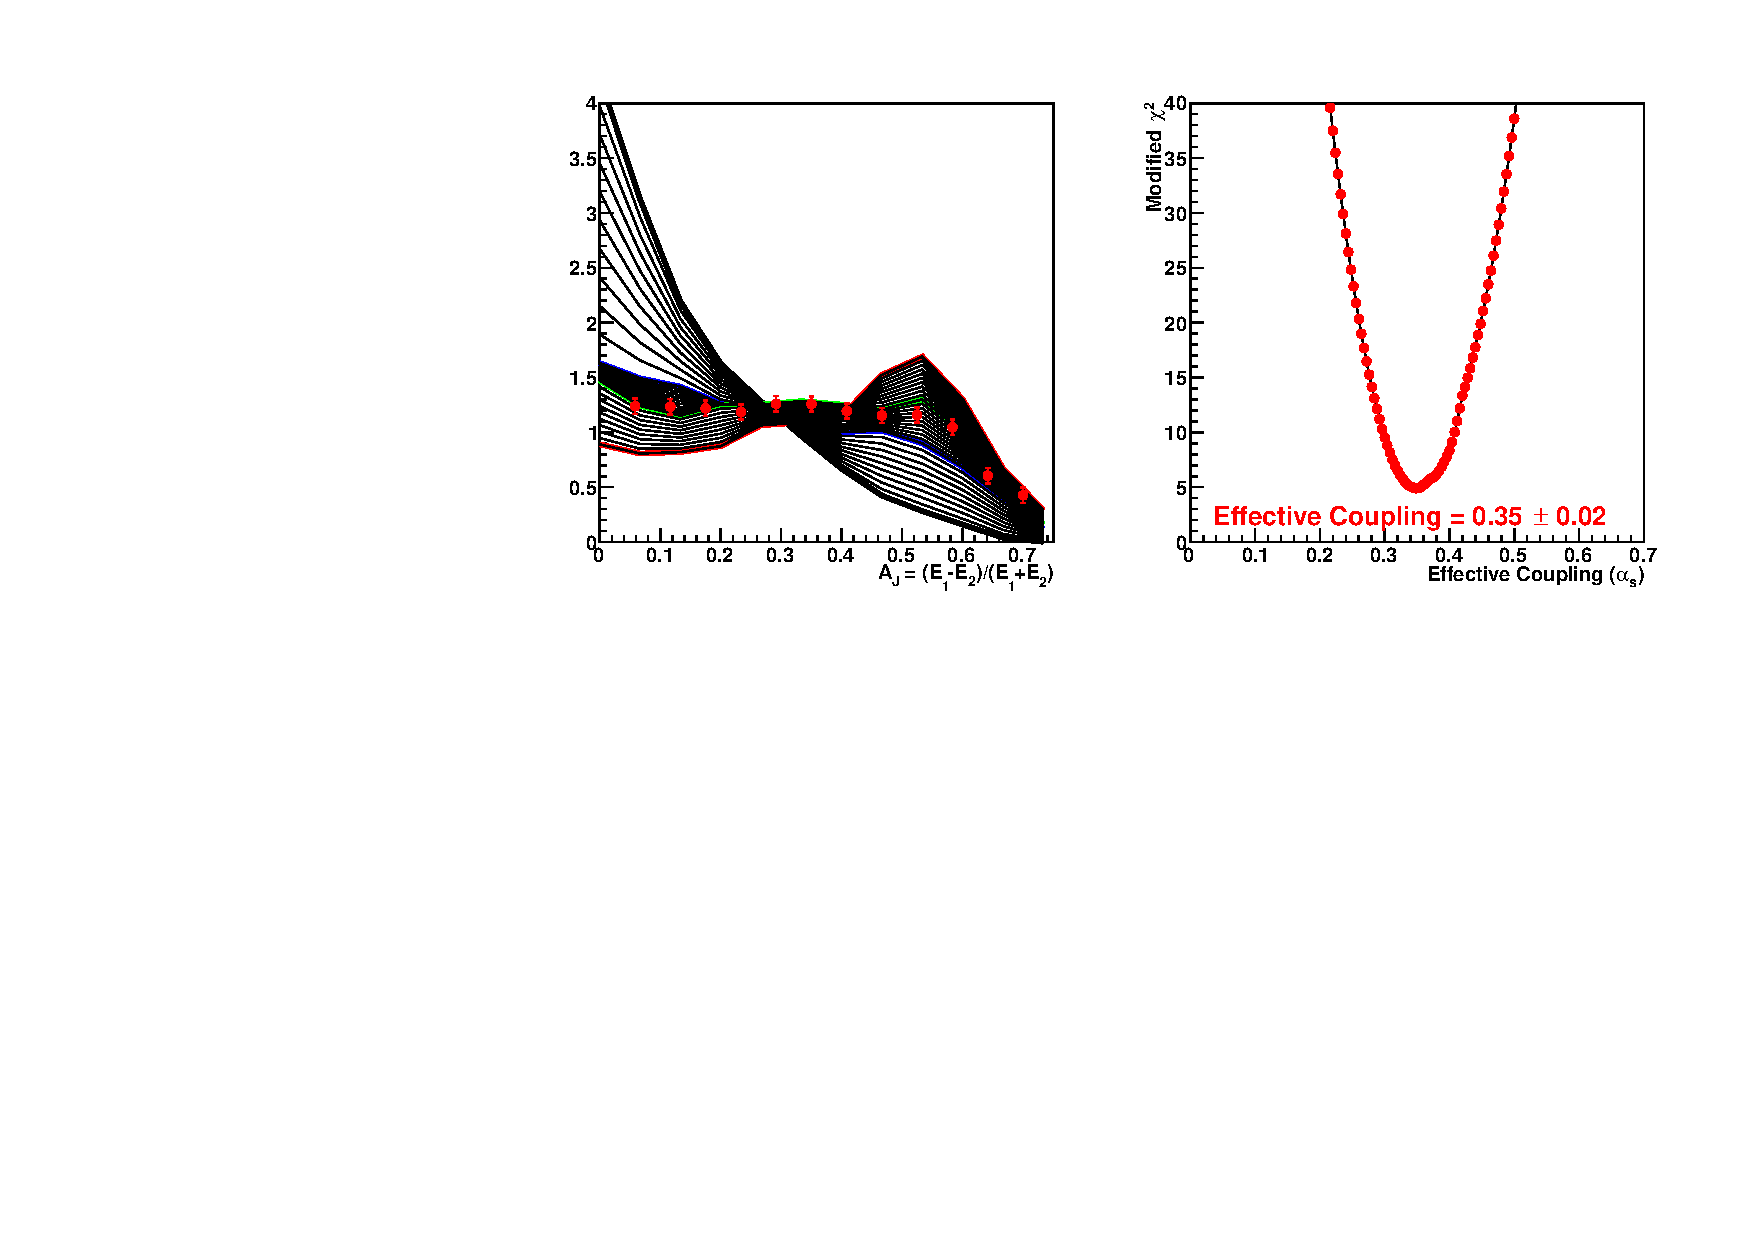
\includegraphics[trim = 10 0 10 0, clip, width=0.98\linewidth]{figs/figure_dijet_constraintalpha}
%    \caption{Determination of effective coupling strength in the model
%      of Coleman-Smith.}
%    \label{fig:coupling_determination}
%\end{figure}

%Figure~\ref{fig:coupling_determination} demonstrates the determination
%of the effective coupling in the model of Coleman-Smith.  The
%different curves in the left panel show the distribution of dijet
%asymmetry for different values of the effective coupling.  The data
%points are generated for a particular value of the coupling strength
%and the uncertainties are representative of those that sPHENIX would
%record.  By performing a modified $\chi_2$ comparison of the model to
%the data, one obtains the curve in the right panel. From that curve,
%one is able to determine the coupling with an uncertainty of about
%5\%.

%\begin{figure}[!hbt]
%  \begin{center}
%    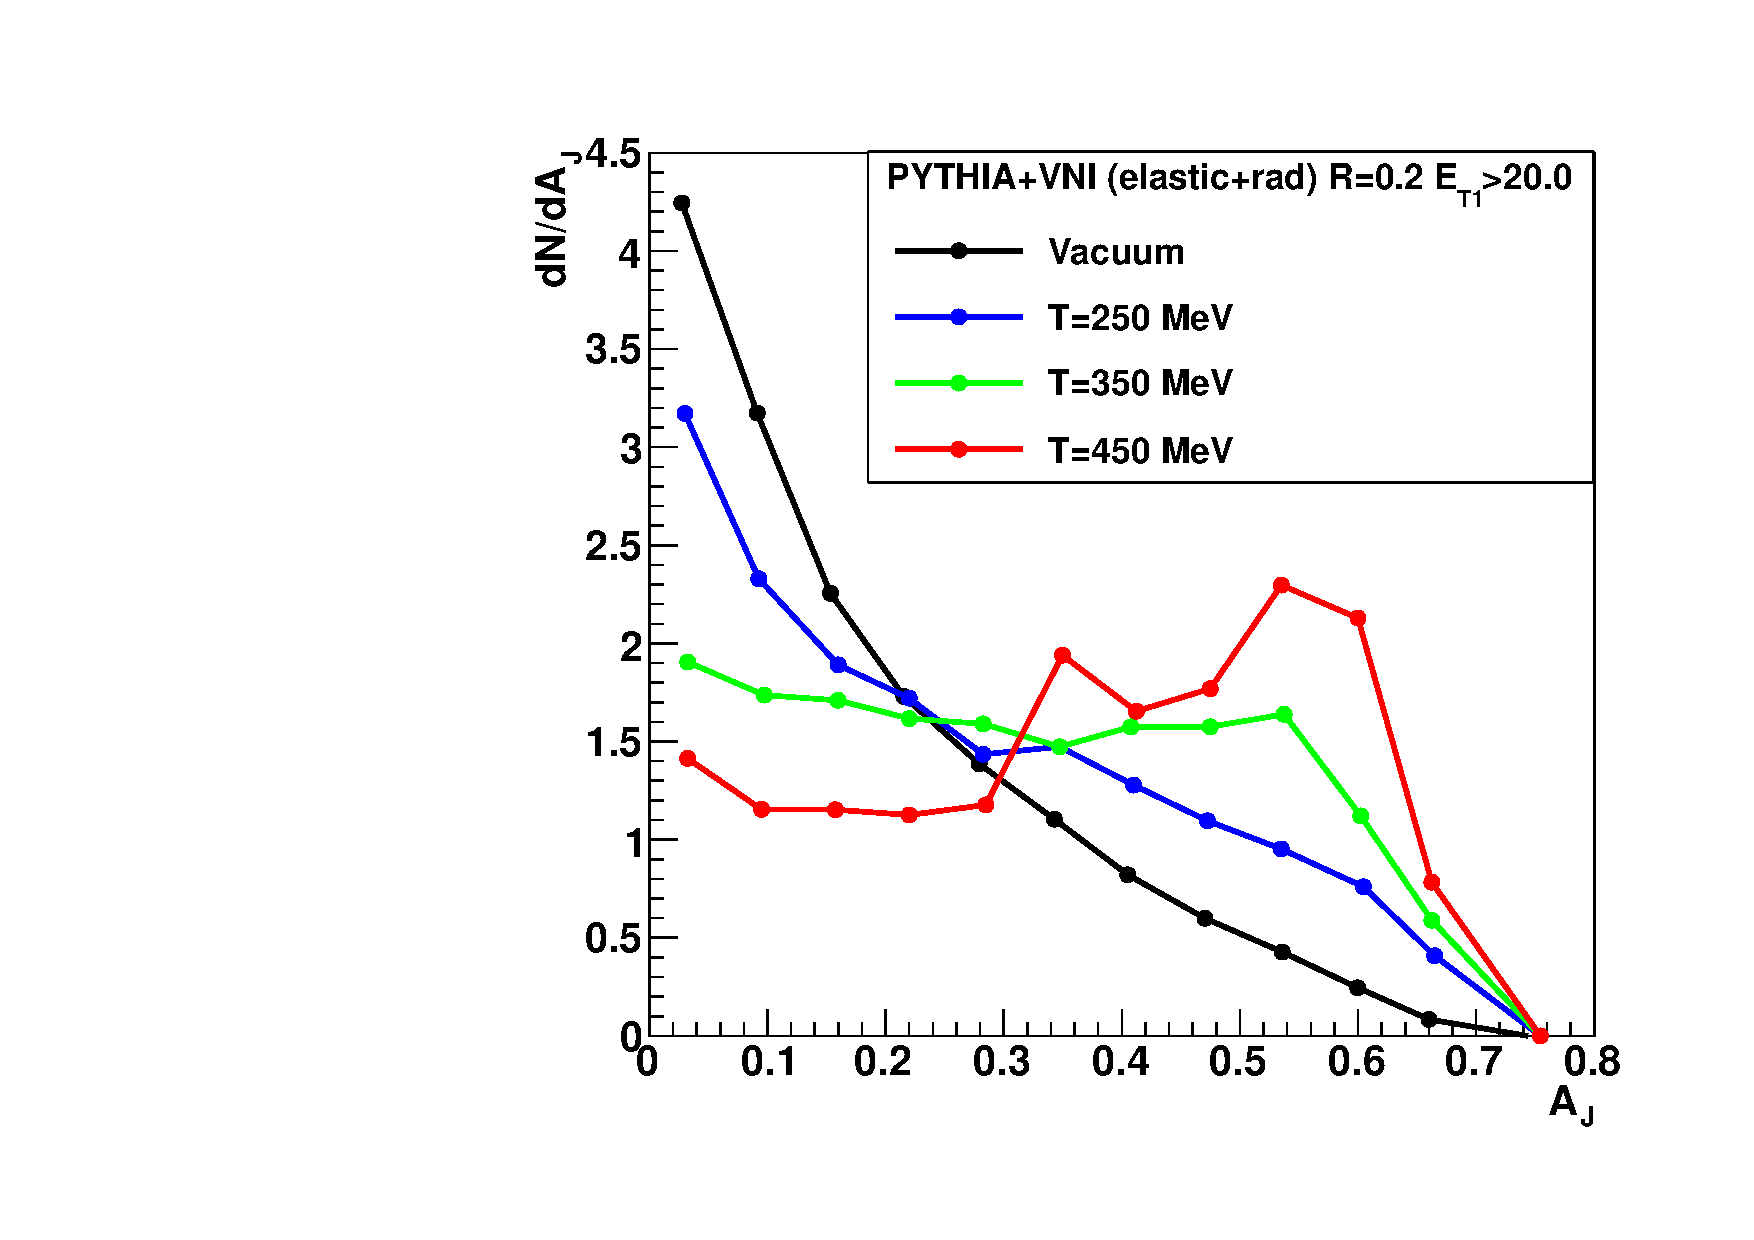
\includegraphics[trim = 2 7 2 2, clip, width=\twowidth]{figs/figure_physicscase_colemansmith_aj_tempdep}
%    \hfill
%    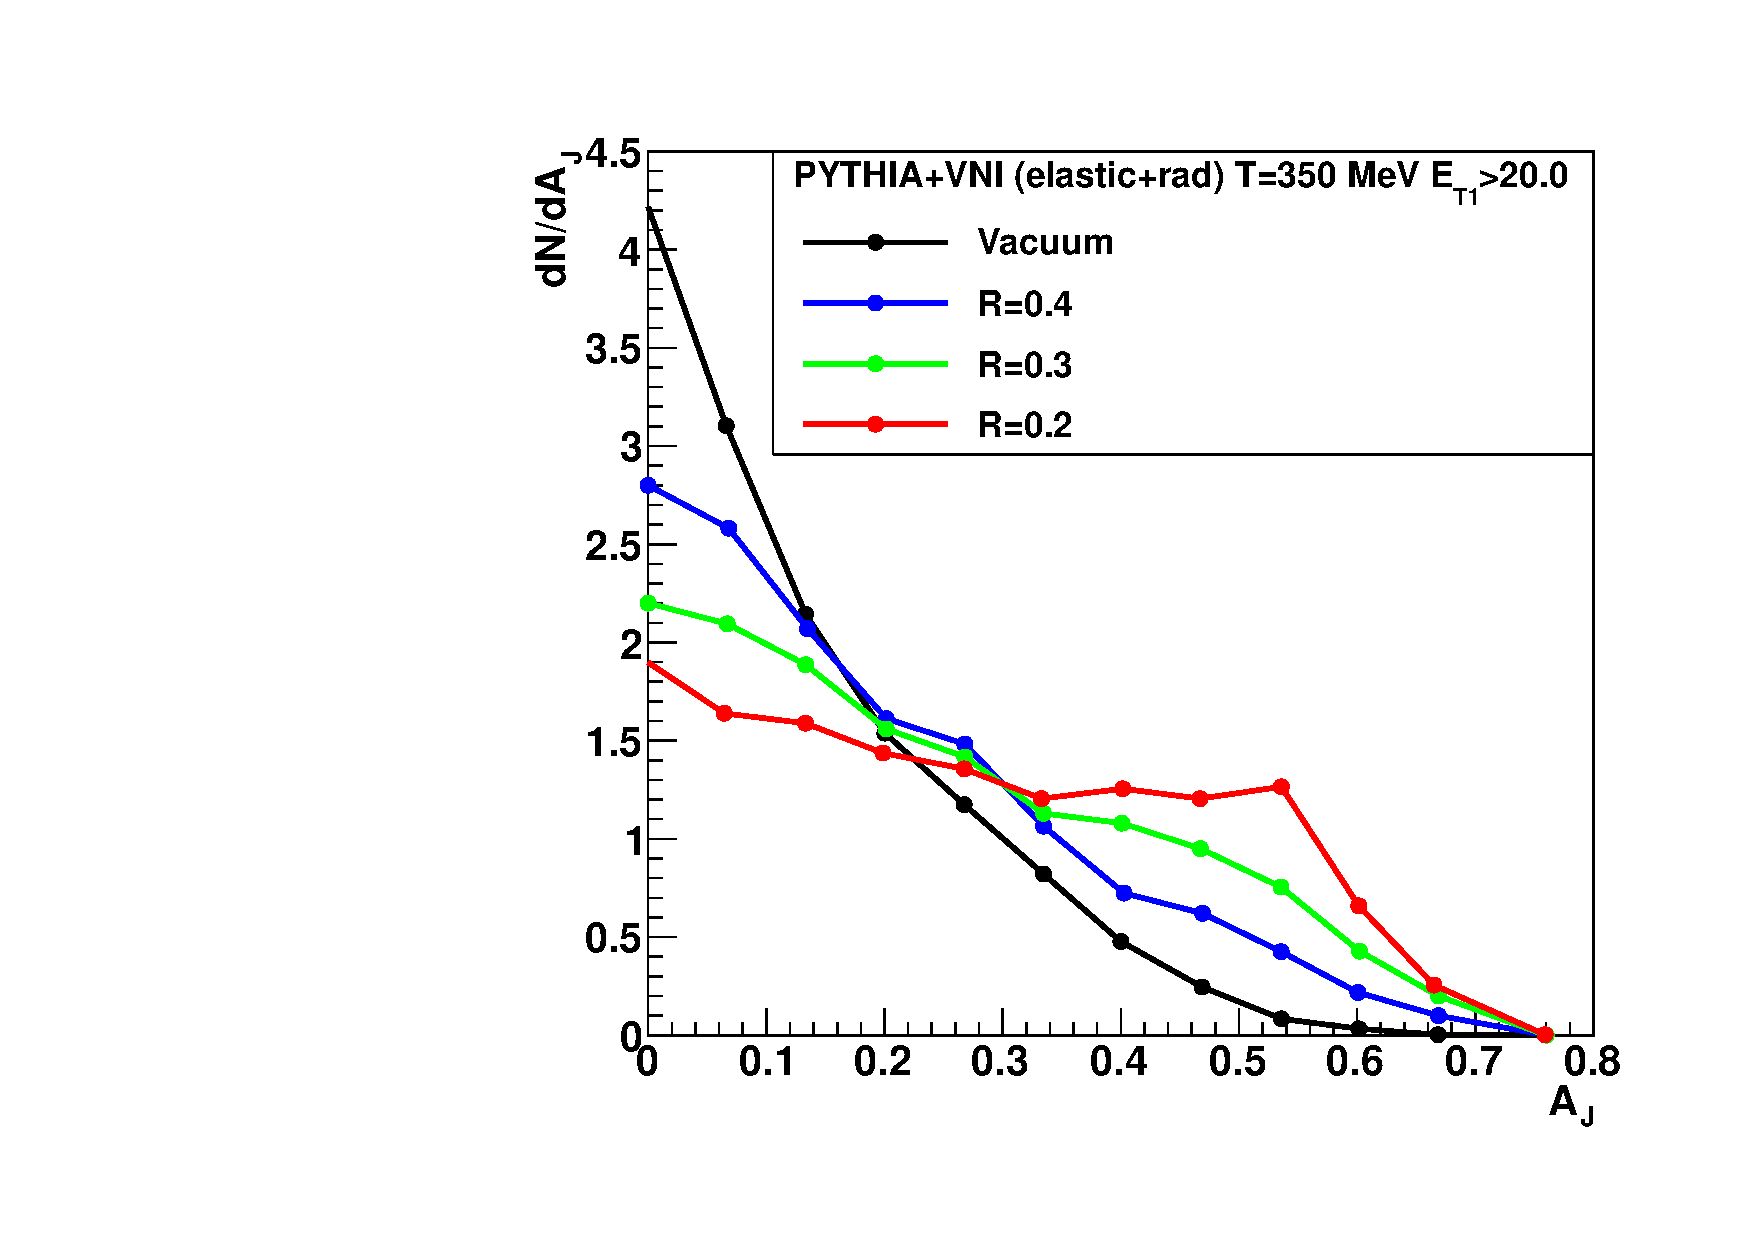
\includegraphics[trim = 2 2 2 2, clip, width=\twowidth]{figs/figure_physicscase_colemansmith_aj_rdep}

%    \caption[Calculation by Coleman-Smith of dijet asymmetry $A_J$ for
%    leading jets with $E_T>20$~GeV as the medium temperature is
%    varied and as the jet cone radius is varied at fixed
%    temperature]{\label{fig:csprobescale}Calculations from
%      Coleman-Smith~\protect\cite{ColemanSmith:2012vr}{} for dijets
%      embedded into the VNI parton cascade.  The dijet asymmetry $A_J$
%      for leading jets with $E_T>20$~GeV is shown as the medium
%      temperature is varied (left panel) and as the jet cone radius is
%      varied with fixed temperature $T=350$~MeV (right panel).}
% \end{center}
%\end{figure}

%Figure~\ref{fig:csprobescale} (left panel) shows the temperature
%dependence of the dijet asymmetry, now keeping the coupling
%$\alpha_{s}$ fixed.  One observes a similar sharp drop in the fraction
%of energy balanced dijets with increasing temperature to that seen for
%increasing the effective coupling, and so combining these observations
%with constrained hydrodynamic models and direct photon emission
%measurements is important.  Given that the initial temperatures of the
%QGP formed at RHIC and the LHC should be significantly different, this
%plot shows that if RHIC and LHC measure the $A_J$ distribution at the
%same jet energy there should still be a sensitivity to the temperature
%which will lead to an observable difference.  Thus, having overlap in
%the measured jet energy range at RHIC and the LHC is important, and
%this should be available for jet energies of 40--70~GeV.
%Figure~\ref{fig:csprobescale} (right panel) shows the jet cone size,
%$R$, dependence of $A_J$ at a fixed temperature.  The narrowest jet
%cone $R=0.2$ has the most modified $A_J$ distribution, as partons are
%being scattered away by the medium to larger angles.

%\begin{figure}[!hbt]
% \begin{center}
%    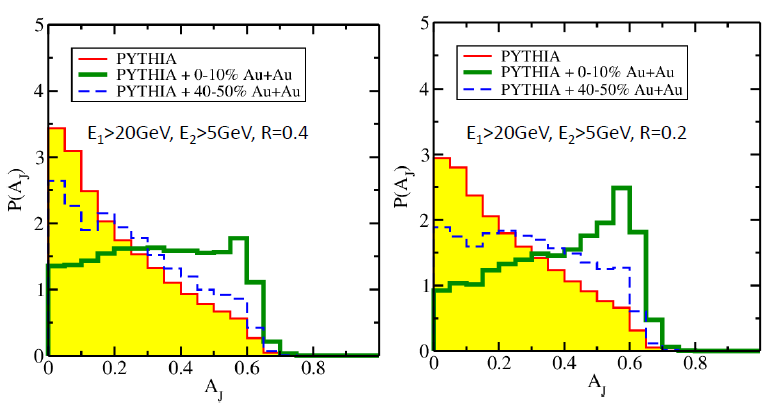
\includegraphics[trim = 2 2 2 2, clip, width=0.8\linewidth]{figs/figure_physicscase_qin_aj_rhic20_04}
%    \caption[Calculations by Qin et al. of dijet $A_{J}$ for
%    $E_{T,1}>20$~GeV and $E_{T,2}>5$~GeV for $R=0.2, 0.4$
%    jets]{\label{fig:qinaj1} Calculations from Qin et
%      al.~\protect\cite{qin_privatecomm}{} of dijet $A_{J}$ for
%      $E_{T,1}>20$~GeV and $E_{T,2}>5$~GeV for $R=0.4$ jets (left)
%      and $R=0.2$ jets (right).  Central (green) and mid-central
%      (blue) distributions are shown along with the initial \pythia
%      distributions (red).}
% \end{center}
%\end{figure}

The second results are from Qin and
collaborators~\cite{Qin:2010mn,qin_privatecomm} where they solve a
differential equation that governs the evolution of the radiated gluon
distribution as the jet propagates through the medium.  Energy
contained inside the jet cone is lost by dissipation through elastic
collisions and by scattering of shower partons to larger angles.
Their calculation is able to describe the LHC measured dijet
asymmetry~\cite{Qin:2010mn}.  

%Figure~\ref{fig:qinaj1} shows the
%predicted dijet asymmetry at RHIC for mid-central and central \auau
%collisions for leading jets $E_{T1} > 20$~GeV and jet radius
%parameter $R=0.4$ and $R=0.2$ in the left and right panels,
%respectively.  Despite the calculation including a rather modest value
%of $\hat{q}$ and $\hat{e}$, the modification for $R=0.2$ is as strong
%as the result with $\alpha_{s} = 0.6$ from Coleman-Smith and
%collaborators shown above in the right panel of
%Figure~\ref{fig:colemansmith1}.  Calculations of $\gamma$-jet
%correlations indicate similar level modifications.  It is also notable
%that Qin and collaborators have calculated the reaction plane
%dependence of the dijet $A_J$ distribution and find negligible
%differences.  This observable will be particularly interesting to
%measure at RHIC since these calculations have difficultly reproducing
%the high $p_T$ $\pi^{0}$ reaction plane dependence ($v_2$) as
%discussed in the previous section.

%Figure~\ref{fig:qinraa} shows results for the inclusive jet \raa
%as a function of $p_T$ for jet radius parameters $R=0.2$ and $R=0.4$.
%It is striking that the modification is almost independent of $p_T$ of
%the jet and there is very little jet radius dependence.  The modest
%suppression, of order 20\%, in mid-central \auau collisions is of
%great interest as previous measurements indicate modification of
%single hadrons and dihadron correlations for this centrality category.
%Measurements of jets with a broad range of radius parameters are
%easier in the lower multiplicity mid-central collisions.

%\begin{figure}[t]
% \begin{center}
%    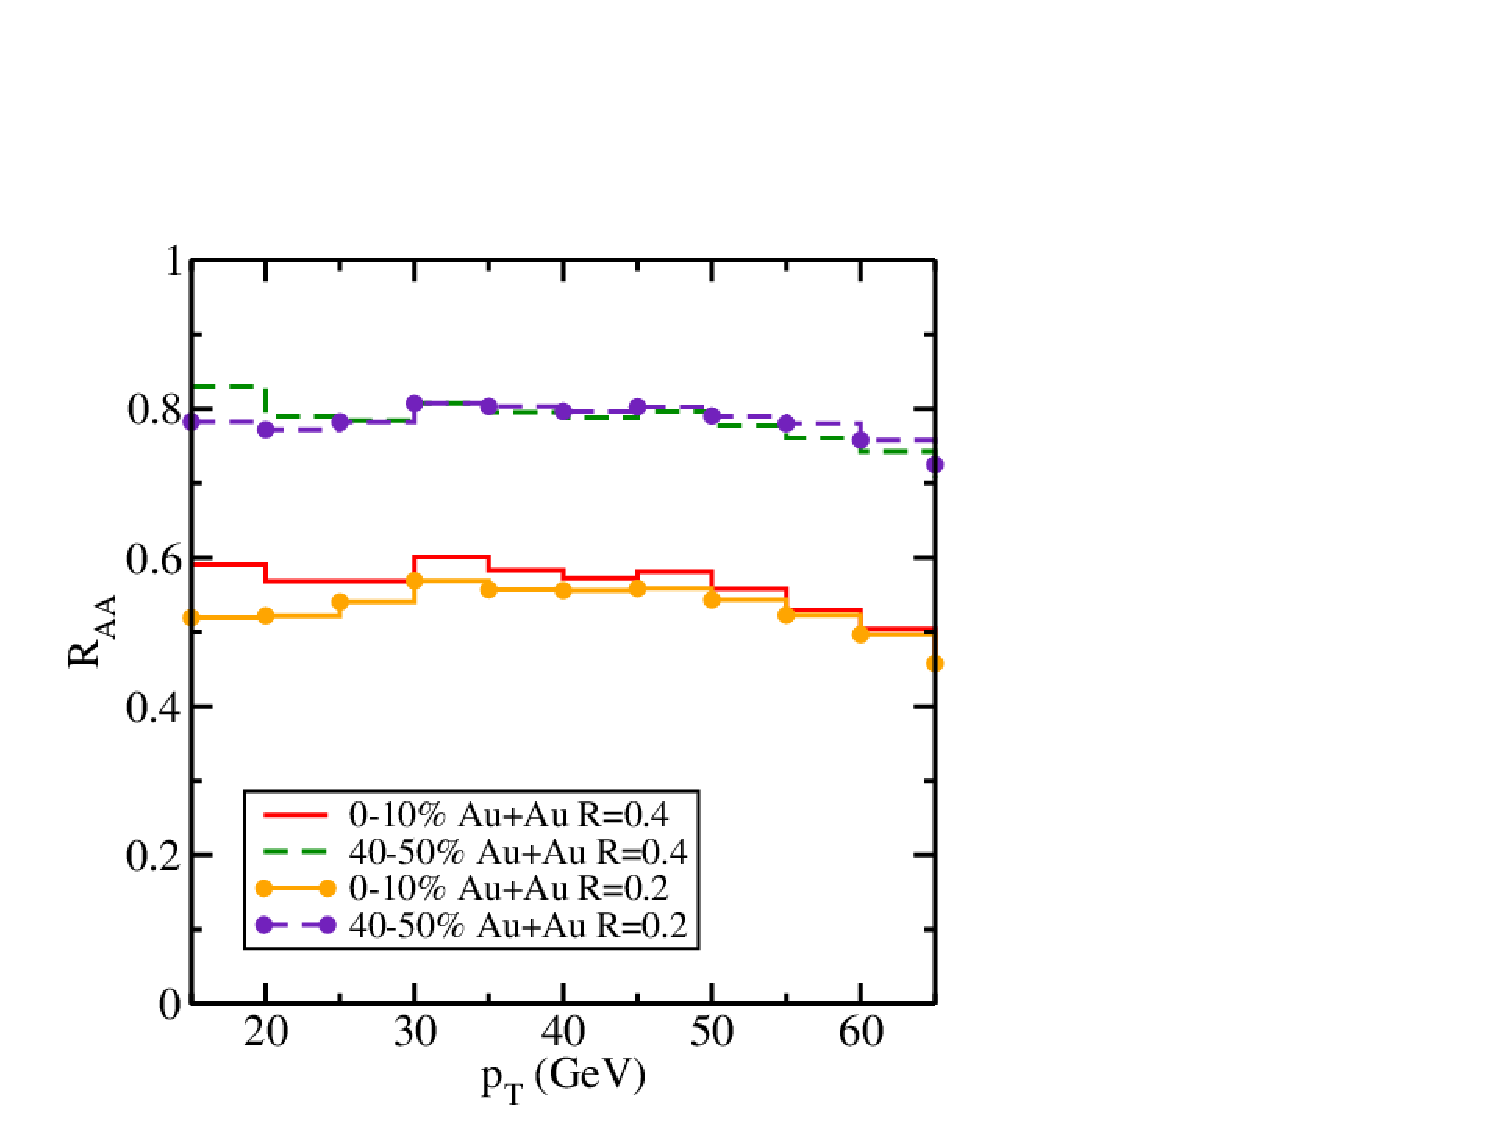
\includegraphics[trim = 2 2 2 2, clip, width=0.5\linewidth]{figs/figure_physicscase_qin_jetraa}
%    \caption[Calculations from Qin et al. of jet \raa for central
%    and mid-central collisions for $R=0.2, 0.4$
%    jets]{\label{fig:qinraa} Calculations from Qin et
%      al.~\protect\cite{qin_privatecomm}{} for jet \raa for
%      central (solid lines) and mid-central collisions (dashed lines)
%      for $R=0.2$ and 0.4 jets.}
% \end{center}
%\end{figure}

The third results are from Young and Schenke and
collaborators~\cite{Young:2011va}.  These calculations utilize a jet
shower Monte Carlo, referred to as \martini~\cite{Schenke:2009vr},
and embed the shower on top of a hydrodynamic space-time background,
using the model referred to as \music~\cite{Schenke:2010nt}.
Figure~\ref{fig:martiniaj} shows the jet energy dependence of $A_J$
for RHIC energy dijets, $E_{T1}>25$~GeV and $E_{T1}>35$~GeV in the
left and right panels, respectively.  These results are directly
compared to the calculations from Qin and collaborators and indicate
a substantially different modification for the higher energy dijets.
Interestingly, both of these approaches, when applied at the higher
collision energies of the LHC, each reproduce the measured data quite
well~\cite{Young:2011qx,Qin:2010mn}.

\begin{figure}[t]
 \begin{center}
    \raisebox{0.08in}{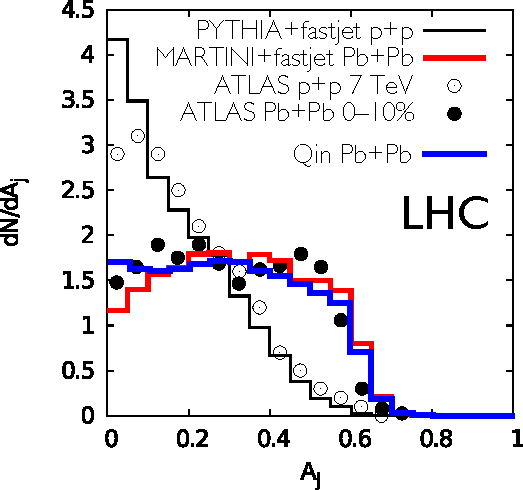
\includegraphics[trim = 0 0 0 0, width=0.48\linewidth]{figs/aj_both}}
%    \includegraphics[trim = 40 0 40 0, clip, width=\twowidth]{figs/martini_music_qin_20_25}
    \hfill
    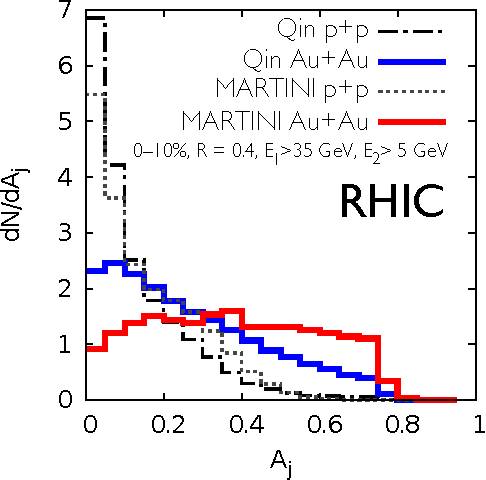
\includegraphics[trim = 0 0 0 0, clip, width=0.47\linewidth]{figs/martini_music_qin_35}
    \caption[$A_J$ distributions in \martinimusic and in the model of
    Qin et al. at LHC and RHIC energies]{\label{fig:martiniaj} $A_J$
      distributions in
      \martinimusic~\protect\cite{Young_privatecomm}{} and the model
      of Qin et al.~\protect\cite{qin_privatecomm}{}.  (left)
      Comparison of $A_J$ calculations in \martinimusic and by Qin et
      al for \pbpb collisions at 2.76~TeV (red line, Qin et al; blue
      line, \martinimusic).  Both calculations show a similar broad
      $A_J$ distribution.  (right) Same as left panel, but for \auau
      collisions at 200~GeV (with leading jet $E_T>35$~GeV).  Here a
      difference in shape is observed between the two models with the
      Qin et al. model developing a peak at small $A_J$ while the
      \martinimusic calculation retains a shape in the calculation at
      the higher energy.}
 \end{center}
\end{figure}

Our next set of illustrative theory calculations come from Vitev and
collaborators~\cite{He:2011pd,Neufeld:2011yh,Vitev:2009rd} where they
utilize a Next-to-Leading-Order (NLO) calculation and consider not only
final-state inelastic parton interactions in the QGP, but also initial-state cold
nuclear matter effects.  
%Figure~\ref{fig:vitevaj} shown earlier plots the dijet asymmetry $A_J$ for jets 
%with $E_{T1} > 50$~GeV and $R=0.6$. 
%The plots are for cases of radiative energy loss only and including collisional energy loss as well,
%and then the different colors are varying the probe-medium coupling by $\pm$10\%.   There is 
%sensitivity even to these 10\% coupling modifications, and for the higher energy jets there is a
%dramatic difference predicted from the inclusion of collisional energy loss. 

For the inclusive jet suppression, these calculations predict a
significant jet radius $R$ dependence to the modification, in contrast
to the result from Qin and collaborators.
Figure~\ref{fig:vitev_raasize} shows the significant radius
dependence.  In addition, Vitev and collaborators hypothesize a
substantial cold nuclear matter effect of initial state parton energy
loss.  Because the high energy jets originate from hard scattering of
high Bjorken $x$ partons, a modest energy loss of these partons
results in a reduction in the inclusive jet yields.  At RHIC with
\dAu~running we will make cold nuclear matter measurements at the same
collision energy and determine the strength of these effects as a
baseline to heavy ion measurements.

\begin{figure}[t]
 \begin{center}
    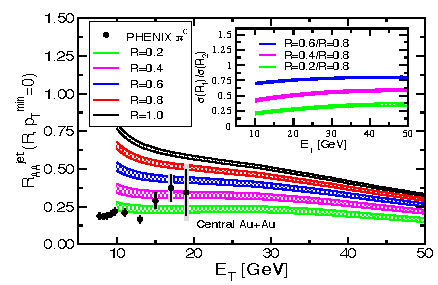
\includegraphics[width=0.6\linewidth]{figs/vitev_auau_RHIC_jetRAA}
    \caption[Calculations by Vitev et al. for the inclusive jet \raa
    vs jet energy and radius]{\label{fig:vitev_raasize} Calculations
      from Vitev et al. for the inclusive jet \raa as a function of
      the jet energy and radius.  }
 \end{center}
\end{figure}

%Recently a framework with a hybrid strong coupling approach has been implemented with initial success at describing
%specific jet quenching observables~\cite{Casalderrey-Solana:2014wca,Casalderrey-Solana:2014bpa}.   Shown in 
%Figure~\ref{fig:uberstrong} are the predicted \raa for reconstructed jets at the LHC (left) and at RHIC (right).   
%The jet \raa shows a rise as a function of \pt at both energies, in contrast to calculations as shown in Figure~\ref{fig:qinraa} for example.
%This framework enables an alternate set of  predictions for a host of observables sensitive to the redistribution
%of energy within the parton shower at RHIC and the LHC.  The steeper spectrum at RHIC and the lower energy jets should
%make them more sensitive to the details of the hybrid calculations.

%\begin{figure}[t]
% \begin{center}
%    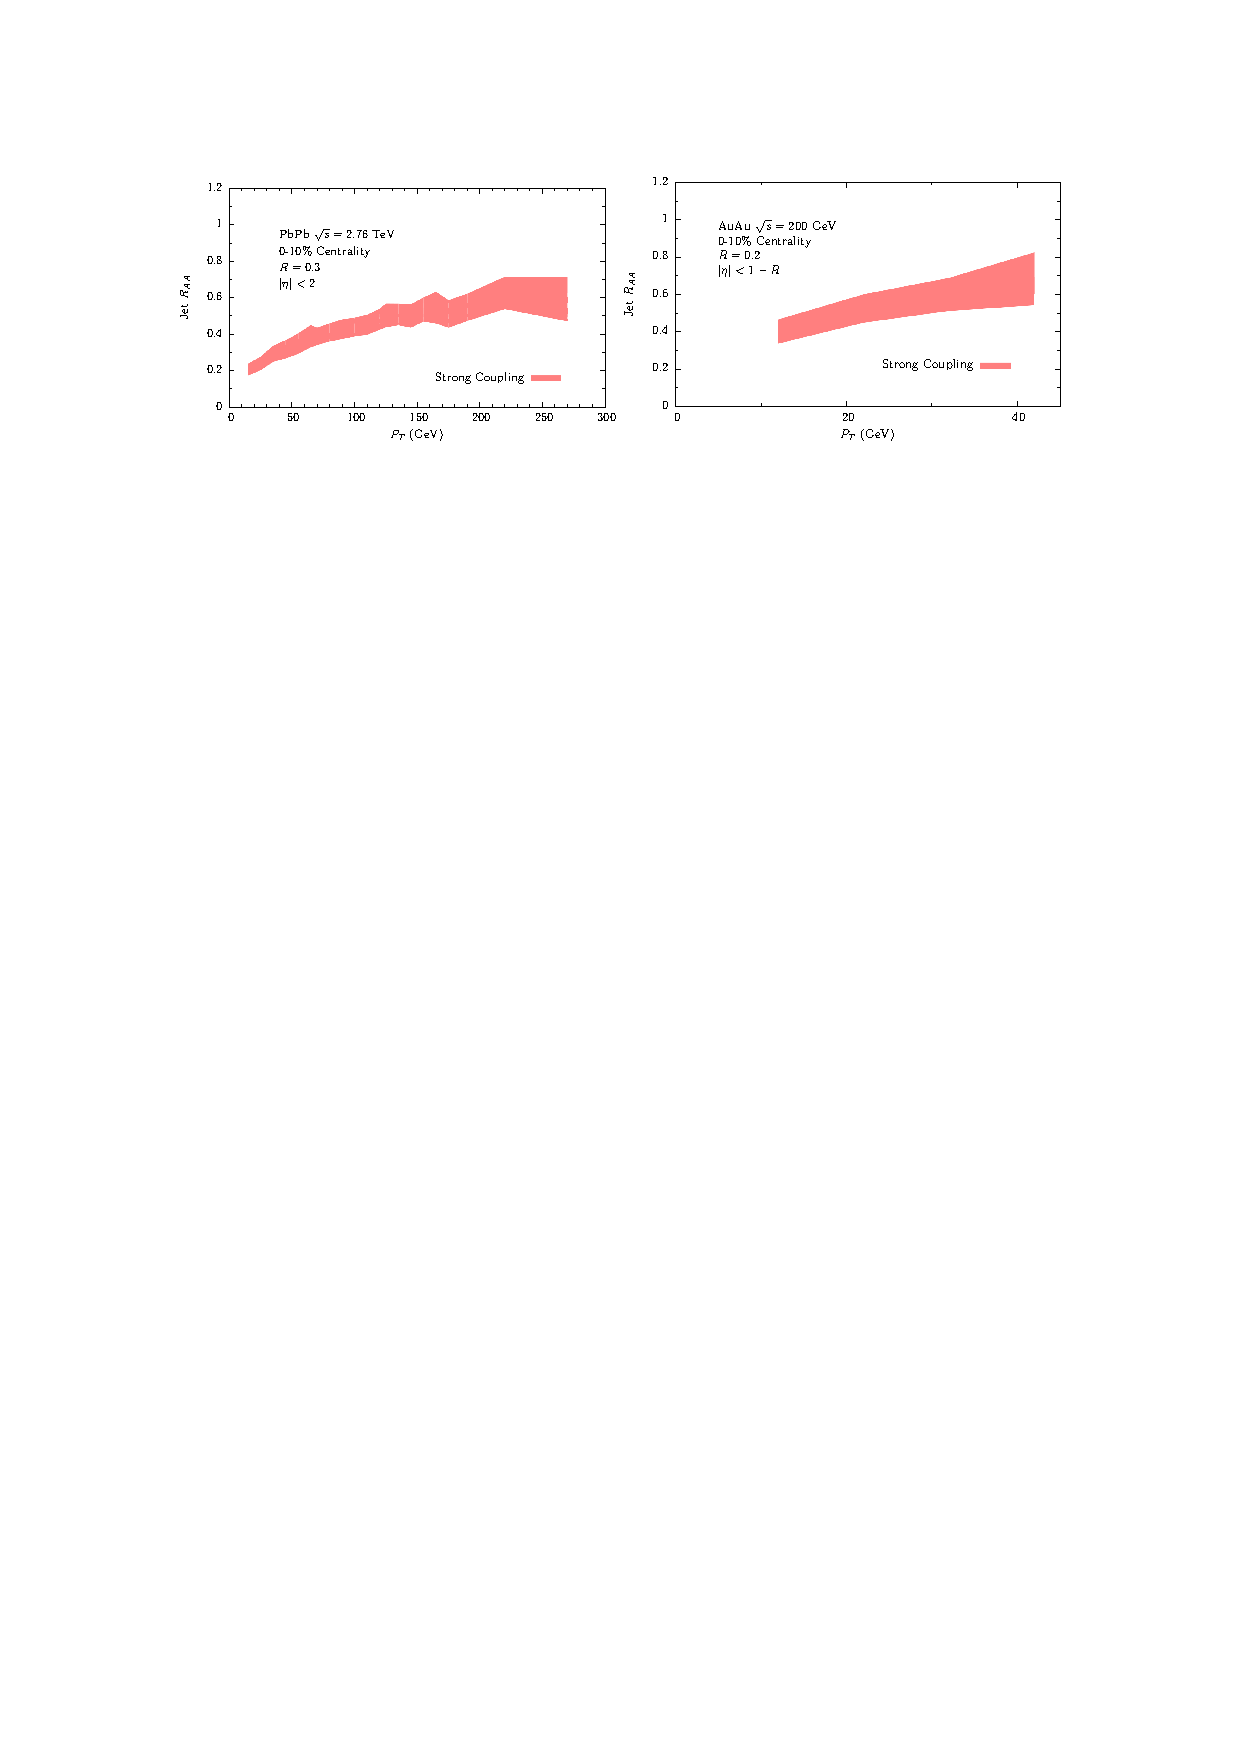
\includegraphics[width=0.95\linewidth]{figs/hybrid_strong_raa}
%    \caption[Calculations of jet \raa vs \pt for central collisions at
%    the LHC and at RHIC using the hybrid strong coupling approach of
%    Casalderrey-Solana et al]{\label{fig:uberstrong} Calculations from
%      a hybrid strong coupling approach with predictions for
%      reconstructed jet \raa as a function of \pt appropriate for
%      central collisions at the LHC (left) and RHIC
%      (right)~\cite{Casalderrey-Solana:2014wca,Casalderrey-Solana:2014bpa}.
%    }
% \end{center}
%\end{figure}

%SEEMS REASONABLE TO REMOVE THE JEWEL PLOT BELOW (?)

%The simultaneous development of parton shower Monte Carlo codes -- for
%example see
%Refs.~\cite{Zapp:2009pu,Renk:2010zx,Young:2011va,ColemanSmith:2011wd,Lokhtin:2011qq,Armesto:2009zc}
%-- and in some cases their public availability allows the community to
%explore a full range of experimental observables.  We have run the
%JEWEL 2.0 code~\cite{Zapp:2013vla} at both RHIC and LHC kinematics and
%medium parameters and then run the HEPMC output through the FASTJET
%reconstruction code.  Results of a suite of observables for both
%energies are shown in Figure~\ref{fig:uberjewel}.  The top panel shows
%the jet \raa for different jet radii and charged hadron \raa.  It is
%striking as pointed out earlier that the charged hadron \raa is quite
%flat at RHIC and at the same time has the characteristic rise at the
%LHC as observed in data.  The next panel shows the modified
%fragmentation function from inclusive jets, where the observable
%reflects both the modification in the parton shower and the
%potentially reduced fraction of energy captured within the
%reconstructed jet.  The next panel shows the dijet azimuthal asymmetry
%with the dashed lines in \pp collisions and the solid lines in central
%heavy ion collisions.  The RHIC predictions show a measurable
%broadening of the azimuthal distribution.  The next panel shows the
%$A_J$ dijet asymmetry distribution.  The steeper falling spectrum at
%RHIC leads to a more significant depletion of balanced jets (i.e. $A_J
%\approx 0$) and a larger shifts in the $\left<A_{J}\right>$.  The
%bottom panel shows the related $I_{AA}$ for dijets, in this case with
%a narrow trigger jet with $R=0.2$ and varying the away-side jet
%radius.  Again, a dramatic modification is expected at RHIC from the
%interplay of both larger surface bias from the trigger jet and a bias
%for the away-side parton to be a gluon opposed a quark trigger parton.
%sPHENIX will have excellent statistics across this breadth of
%observables and more.

%It is notable that in the recommended running mode for JEWEL, one
%retains recoil partons for hadron reconstruction and not for jet
%reconstruction.  JEWEL treats the medium partons as a gas of nearly
%free quarks and gluons and thus it is relatively easy to transfer
%energy to these partons, which then recoil.  In the case where recoil
%partons are included in the jet reconstruction they have also their
%initial thermal energy and thus one gets large jet \raa enhancements.
%When excluding them, some energy is lost and \raa for large radius
%jets appears smaller than expected.  We are working on a running mode
%to only include the transferred energy and thus test the sensitivity
%to the model of the medium partons.  We continue to directly engage
%the theory community for development of these Monte Carlo codes for
%optimal comparison between data and theory.

%\begin{figure}[t]
% \begin{center}
%    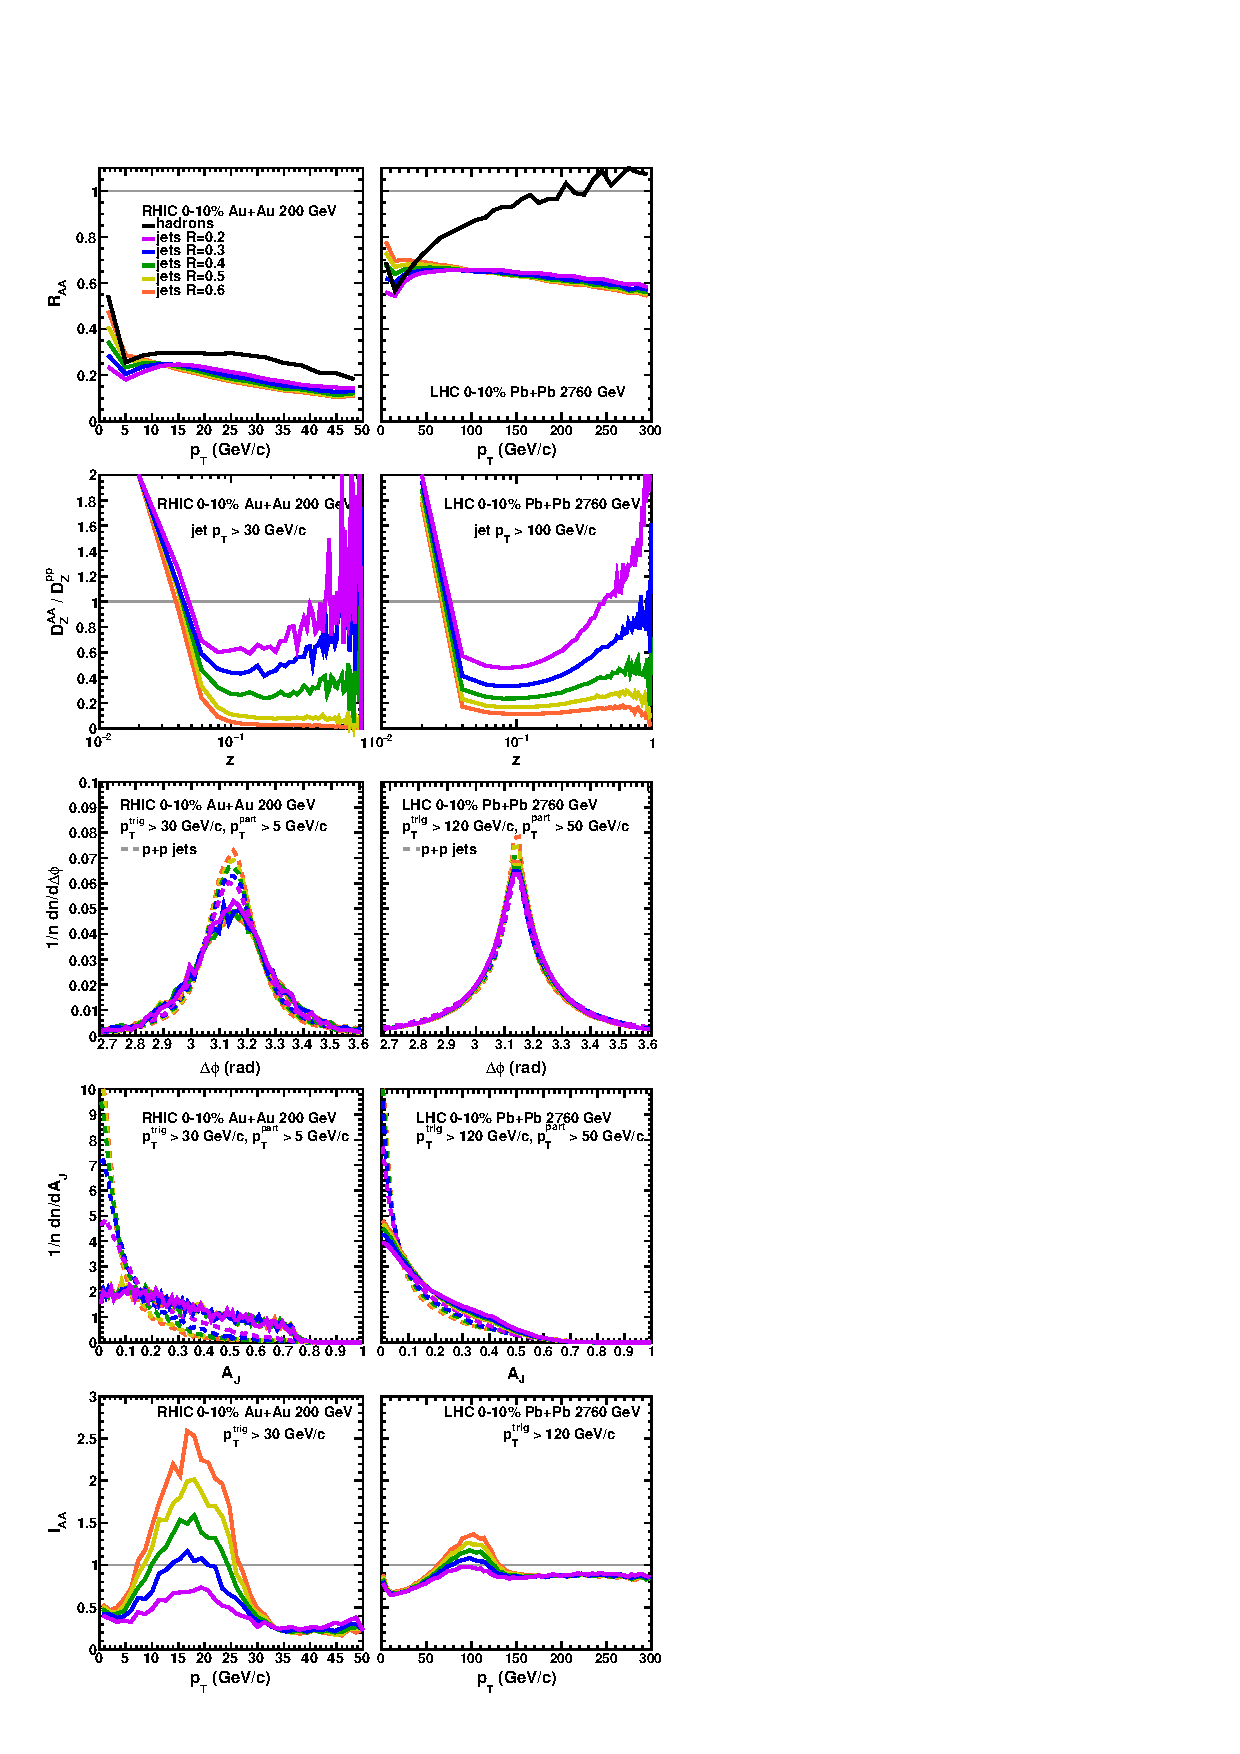
\includegraphics[height=0.9\textheight]{figs/jewel_summary}
%    \caption[Compilation of results for jet and hadron observables at
%    RHIC and the LHC using the JEWEL parton shower Monte
%    Carlo]{\label{fig:uberjewel} JEWEL 2.0 parton shower Monte Carlo
%      results for jet and hadron observables at RHIC and the LHC using
%      the publicly available code~\cite{Zapp:2013vla,Zapp:2008gi}.
%      See text for the detailed description of the panels.  }
% \end{center}
%\end{figure}

%\clearpage

\section{Direct Photons and Fragmentation Functions}
\label{sec:direct_photons_and_ff}

Ideally, one would like to understand how a quark or gluon of
perfectly known energy interacts traversing the \qgp and the
redistribution of energy and particles both longitudinal and
transverse to the initial parton direction.  The \emph{golden channel}
for the calibration of initial quark energy is to tag them via an
opposing direct photon~\cite{Wang:1996yh}.  One can measure fully
reconstructed jets opposite the photon with different jet radii to
parse out the transverse energy redistribution.

Figure~\ref{fig:vitevgammajet} shows the event distribution for the
ratio of the reconstructed jet energy with $R=0.3$ relative to the
direct photon energy~\cite{Dai:2012am}.  As the authors note, ``The
steeper falling cross sections at RHIC energies lead not only to a
narrow $z_{J_{\gamma}}$ distribution in \pp collisions but also to a
larger broadening end shift in $\left<z_{J_{\gamma}}\right>$ in A+A
collisions.''  This results in a greater sensitivity to the
redistribution of energy, which is again sensitive to the balance of
processes including radiative and collisional energy loss.

%Figure~\ref{fig:vitev_gammajet_raa} shows the jet \raa opposite a
%35~GeV direct photon~\cite{Dai:2012am}.  There is a dramatic
%difference between the RHIC and LHC result, where one expects a factor
%of two enhancement in jets near 20~GeV in these collision systems.  
As detailed in the sPHENIX performance section in
Figure~\ref{fig:g4_photon_iaa}, with an underlying event energy a
factor of 2.5 lower at RHIC compared to the LHC, sPHENIX can
reconstruct jets over a very broad range of radii and energies
opposite these direct photons.

\begin{figure}[!hbt]
 \begin{center}
   \raisebox{0.03cm}{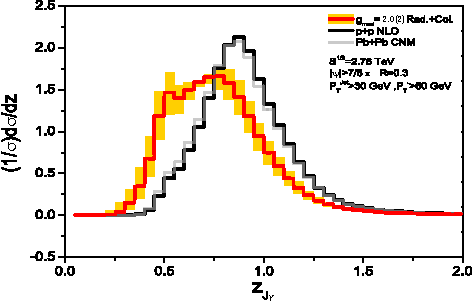
\includegraphics[width=0.50\linewidth]{figs/vitev_gammajet_LHC}}
   \hfill
   \includegraphics[width=0.48\linewidth]{figs/vitev_gammajet_RHIC}
   \caption[Calculations by Vitev et al. of the vacuum and medium
   modified distribution for direct photon triggered reconstructed jet
   events at LHC and RHIC energies]{\label{fig:vitevgammajet}
     Calculation results for the vacuum and medium modified
     distribution for direct photon --- reconstructed jet events at
     LHC collision energy (left) and RHIC collision energy
     (right)~\cite{Dai:2012am}.  }
 \end{center}
\end{figure}

%\begin{figure}[!hbt]
% \begin{center}
%   \includegraphics[width=0.6\linewidth]{figs/vitev_gammajet_raa}
%   \caption[Calculations by Vitev et al. of the jet \raa opposite to a %tagged
%     direct photon in \auau collisions at 200~GeV and \pbpb collisions
%     at 2.76~TeV]{Calculation results for the jet \raa opposite to a tagged
%     direct photon in \auau collisions at 200~GeV and \pbpb collisions
%     at 2.76~TeV~\cite{Dai:2012am}.}
%  \label{fig:vitev_gammajet_raa}
% \end{center}
%\end{figure}

With charged particle tracking one can also measure the longitudinal
redistribution of hadrons opposite the direct photon.  sPHENIX will
have excellent statistical reach for such direct photon measurements.
At the same time, it is advantageous to measure modified fragmentation
functions within inclusive reconstructed jets and via correlations as
well.  The original predictions of jet quenching in terms of induced
forward radiation had the strongest modification in the longitudinal
distribution of hadrons from the shower (i.e., a substantial softening
of the fragmentation function).  One may infer from the nuclear
suppression of $\pi^{0}$ in central \auau collisions $R_{AA} \approx
0.2$ that the high $z$ (large momentum fraction carried by the hadron)
showers are suppressed.  

%Shown in Figure~\ref{fig:fragz} is the
%fragmentation function for 40~GeV jets in vacuum (\pythia) compared
%with the case of substantial jet quenching (Q-\pythia with a quenching
%factor used to match RHIC single hadron suppression observables).  

In the sPHENIX upgrade, fragmentation functions via precision charged
track measurements are available from high-$z$ where the effects are
predicted to be largest to low-$z$ where medium response and
equilibration effects are relevant.  The independent measurement of
jet energy (via calorimetry) and the hadron $p_T$ via tracking is
crucial.  This independent determination also dramatically reduces the
\fake track contribution by the required coincidence with a high
energy jet.

%\begin{figure}[!hbt]
% \begin{center}
%    \includegraphics[width=0.85\linewidth]{figs/figure_decade_frag_z}
%    \caption[Q-\pythia simulation with quenching parameter $\hat{q} =
%    0$ and $\hat{q} = 10$~GeV/c$^{2}$ for the fragmentation function
%    of light quark and gluon jets as a function of $z$.
%    ]{\label{fig:fragz}Q-\pythia simulation with quenching parameter
%      $\hat{q} = 0$ (i.e., in vacuum) and $\hat{q} = 10$~GeV/c$^{2}$
%      for the fragmentation function of light quark and gluon jets as
%      a function of $z$.  }
% \end{center}
%\end{figure}

%Measurements at the LHC reveal a very different behavior as shown in %Figure~\ref{fig:LHC_FF_measurements} where
%a slight enhancement is hinted at for large $z$, rather than a large suppression.
%Measurements of fragmentation functions within reconstructed jets from the CMS and
%ATLAS experiments in \pbpb collisions show very modest modification within
%uncertainties. Although one explanation is that the jets that are
%reconstructed are from near the surface and thus not modified, with a
%nuclear modification factor for inclusive jets $R_{AA} \approx 0.5$
%that explanation is challenged.   Similar measurements at RHIC energies
%are crucial to fully map out the re-distribution of energy in the shower
%and medium response.   An example of the sPHENIX precision for such measurements is shown 
%later in Figure~\ref{fig:fastsim_ff}.

%\begin{figure}[!hbt]
% \begin{center}
%   \raisebox{3.5ex}{\includegraphics[width=0.45\linewidth]{figs/ATLAS_PbPb_FF}}
%   \includegraphics[width=0.51\linewidth]{figs/CMS_PbPb_FF} 
%   \caption[The modified fragmentation function for $p_\mathrm{T} >
%   100$~GeV jets in central Pb+Pb collisions vs $z$ from ATLAS and vs
%   $\xi$ from CMS]{\label{fig:LHC_FF_measurements} Measurements of the
%     modified fragmentation function for $p_\mathrm{T} > 100$~GeV jets
%     in central Pb+Pb collisions from ATLAS~\cite{Aad:2014wha} (left
%     plot, as a function of $z = \vec{p}_\mathrm{T}^\mathrm{\
%       hadron}\cdot\vec{p}_\mathrm{T}^\mathrm{\ jet} /
%     \left|\vec{p}_\mathrm{T}^\mathrm{\ jet}\right|^{2}$) and
%     CMS~\cite{Chatrchyan:2014ava} (right plot, as a function of $\xi
%     = 1/z$).  } \end{center}
%\end{figure}

One can also access less directly this transverse and longitudinal redistribution of energy and particles
via trigger high \pt hadrons and narrow reconstructed jets.    Similar measurements have been carried out by
the STAR experiments, as discussed earlier in the context of Figure~\ref{fig:star_hjet}.   
With the large kinematic reach of sPHENIX, 
one can have very high statistics observables that span a reach where the opposing parton is mostly a gluon near 20~GeV and then
increases in quark fraction for higher energy triggers.   This is another complement between the kinematics at RHIC
and the LHC as shown in Figure~\ref{fig:partonfrac} comparing the quark-quark, quark-gluon, gluon-gluon relative contributions
as a function of \pt.

\begin{figure}[!hbt]
 \begin{center}
    \includegraphics[width=0.7\linewidth]{figs/figure_jetfraction_rhiclhc}
\caption{Comparison of the fraction of quark and gluon jets from leading order pQCD calculations for RHIC and LHC energies.
\label{fig:partonfrac}}
\end{center}
\end{figure}

%Combining high statistics results on this full set of observables from
%RHIC and the LHC can lead to a detailed description of the quark and
%gluon interaction in the \qgp as a function of parton energy analogous
%to that from the Particle Data Group for the muon in copper as shown
%in Figure~\ref{fig:mucu}.

%\begin{figure}[!hbt]
% \begin{center}
%    \includegraphics[width=0.7\linewidth]{figs/mucu_color.png}
%    \caption[The muon stopping power in copper]{The muon stopping
%      power in copper demonstrates a comprehensive understanding of
%      the interaction of a fundamental particle with matter over an
%      enormous range of scales.\label{fig:mucu}}
%\end{center}
%\end{figure}

%\clearpage

\section{Heavy Quark Jets}
\label{sec:heavyquark}

A main motivation for studying heavy flavor jets in heavy ion
collisions is to understand the mechanism for parton-medium
interactions and to further explore the issue of {\it strong versus weak} coupling~\cite{horowitz}.  
As detailed in Section~\ref{Section:InnerWorkings}, a major goal is understanding the constituents of the medium
and how fast partons transfer energy to the medium.   Heavy quarks have gathered special attention as they are 
particularly sensitive to the contribution of collisional energy loss, due to suppressed radiative energy loss from the
``dead cone'' effect~\cite{dk_dead_cone}.   Measurements of beauty-tagged jets and reconstructed $D$ mesons over the broadest
kinematic reach will enable the disentangling of $\hat{q}$ and $\hat{e}$.   

There are important measurements currently being made of single electrons from semileptonic $D$ and $B$ decays and direct $D$ meson 
reconstruction with the current PHENIX VTX and STAR Heavy Flavor Tracker (HFT).  The sPHENIX program can significantly expand 
the experimental acceptance and physics reach by having the ability to reconstruct full jets with a heavy flavor tag.
The rates for heavy flavor production from perturbative QCD calculations~\cite{Cacciariprivate} are shown in 
Figure~\ref{fig:heavyrates}.

\begin{figure}[!hbt]
 \begin{center}
    \includegraphics[width=0.7\linewidth]{figs/fig_pqcdrates_heavyflavor_auau}
    \caption[FONLL calculations of heavy flavor jets, fragmentation
    hadrons, and decay electrons vs \pt]{\label{fig:heavyrates}FONLL
      calculations~\cite{Cacciariprivate} for heavy flavor (charm and
      beauty) jets, fragmentation hadrons ($D, B$ mesons primarily),
      and decay electrons as a function of transverse momentum.  The
      rates have been scaled to correspond to counts with $p_{T} >
      p_{T}(cut)$ for \auau 0--20\% central collisions.}
 \end{center}
\end{figure}

Calculations including both radiative and collisional energy loss for
light quark and gluon jets, charm jets, and beauty jets have been
carried out within the CUJET 2.0 framework~\cite{Xu:2014ica}.  The
resulting \raa values in central \auau at RHIC and \pbpb at the LHC
for $\pi, D, B$ mesons are shown as a function of \pt in
Figure~\ref{fig:cujet}.  The mass orderings are a convolution of
different initial spectra steepness, different energy loss mechanisms,
and final fragmentation.  Measurements of $D$ mesons to high \pt and
reconstructed beauty-tagged jets at RHIC will provide particularly
sensitive constraints in a range where, due to their large masses, the
charm and beauty quark velocities are not near the speed of light.

\begin{figure}[!hbt]
 \begin{center} \includegraphics[width=0.95\linewidth]{figs/CUJET_flavor_RAA_RHIC_LHC} 
   \caption[CUJET calculations of $R_\mathrm{AA}$ in central \auau
   collisions at RHIC and in Pb+Pb collisions at the LHC, with light,
   charm and beauty hadrons and electrons shown as separate
   curves.]{Calculations within the CUJET 2.0~\cite{Xu:2014ica}
     framework of the $R_\mathrm{AA}$ in central Au+Au collisions at
     RHIC (left panel) and Pb+Pb collisions at the LHC (right panel),
     with light, charm and beauty hadrons and electrons shown as
     separate curves.  }
  \label{fig:cujet}
 \end{center}
\end{figure}

%\begin{figure}[!hbt]
% \begin{center} \includegraphics[width=0.55\linewidth]{figs/vitev_b_jet_raa}
%   \caption[Calculations by Vitev et al. of beauty tagged jets showing
%   the sensitivity to radiative and collisional energy loss
%   contributions]{Calculations from Ref.~\cite{Huang:2013vaa} are
%     shown for beauty tagged jets showing the sensitivity to radiative
%     and collisional energy loss contributions.  }
%  \label{fig:bsup}
% \end{center}
%\end{figure}

%Shown in Figure~\ref{fig:bsup} are calculations from
%Ref.~\cite{Huang:2013vaa} that highlight the sensitivity of beauty
%quark jets to collisional energy loss mechanisms.  Initial
%measurements from the LHC show first indications of this mass
%ordering, and precision data from higher statistics in future LHC
%running and at RHIC are needed.  One expects larger effects at RHIC
%where radiative energy loss contributions for the lower \pt beauty
%quarks are suppressed.  Another promising tool is the study of heavy
%flavor jet-shape modification in \auau relative to \pp collisions.
%Different mechanisms of energy loss (radiative versus collisional)
%predict different re-distributions of the jet fragments both inside
%and outside the jet cone.  There are also scenarios where the heavy
%meson forms inside the medium and is dissociated in the
%matter~\cite{Adil:2006ra,Sharma:2009hn}.  This would lead to a nearly
%unmodified jet shape relative to \pp collisions and a much softer
%fragmentation function for the leading heavy meson.

%Figure~\ref{fig:charmfrag} shows the D meson fragmentation function in
%\pythia and Q-\pythia for 20~GeV charm jets.  The peak of the
%fragmentation function is shifted in Q-\pythia from $z \approx 0.7$ to
%$z \approx 0.5$.  Thus, for a given $p_{T}$, $D$ mesons are more
%suppressed than charm jets. Measurement of D mesons within a reconstructed %jet
%will provide access to fragmentation function modifications with
%emphasis on effects at large z.  % to a very nice kinematics.

%\begin{figure}[!hbt]
% \begin{center}
%    \includegraphics[width=0.7\linewidth]{figs/fig_sickles_D_ff_4_ckin20}
%    \caption[$D$ meson fragmentation function in \pythia and Q-\pythia
%    for anti-$k_{T}$ jets with $R = 0.4$ and $E_{T}^\mathrm{jet} > 20$~GeV %as
%    a function of $z$]{\label{fig:charmfrag} $D$ meson fragmentation
%      function in \pythia (open points) and Q-\pythia (solid points)
%      for anti-$k_{T}$ jets with $R = 0.4$ and $E_{T}(jet) > 20$~GeV
%      as a function of $z$, the fractional momentum of the $D$ meson
%      relative to the charm quark.  }
% \end{center}
%\end{figure}

The tagging of charm and beauty jets has an extensive history in
particle physics experiments.  There are multiple ways to tag heavy
flavor jets.  First is the method of tagging via the selection of a
high $p_{T}$ electron with a displaced vertex inside the jet.  In
minimum bias \auau collisions at $\sqrt{s_{NN}} = 200$~GeV, the
fraction of inclusive electrons from $D$ and $B$ meson decays is
already greater than 50\% for $p_{T} > 2$~GeV/c.  The sPHENIX tracking
can confirm the displaced vertex of the electron from the collision
point, further enhancing the signal.  Since the semileptonic branching
fraction of $D$ and $B$ mesons is approximately 10\%, this method
provides a reasonable tagging efficiency.  Also, the relative angle of
the lepton with respect to the jet axis provides a useful
discriminator for beauty jets as well, due to the decay kinematics.
Second, the direct reconstruction of $D$ mesons is possible within
sPHENIX as detailed in the performance section.  The third method
utilizes jets with many tracks that do not point back to the primary
vertex.  This technique is detailed by the $D0$ collaboration to
identify beauty jets at the Tevatron~\cite{d0_nim}, and employed with
variations by ATLAS and CMS at the LHC.  This method exploits the fact
that most hadrons with a beauty quark decay into multiple charged
particles all with a displaced vertex.  The detailed performance
metrics for tagged beauty jets are given in Section~\ref{sec:hqjets}.

As detailed in Ref.~\cite{Huang:2013vaa}, beauty tagged jets at the
LHC come from a variety of initial processes.  In fact, most often a
tagged beauty jet does not have a back-to-back partner beauty jet.  
%As shown in Figure~\ref{fig:bjet_process_fraction}, 
At RHIC energies the
pair creation process represents $\sim35\%$ of the beauty jet
cross-section, which is a larger fractional contribution than at the
LHC, though flavor excitation still produces $\sim50\%$ of all $b$-jets
at RHIC.
Measurements at RHIC offer a different mixture of initial processes,
and thus kinematics, when looking at correlated back-to-back jets
including heavy flavor tags.

%\begin{figure}[hbt!]
%  \centering \includegraphics[width=0.6\textwidth]{figs/sPHENIX_MIE_bjet_process_fraction}
%  \caption[Fraction of inclusive $b$-jets, as a function of jet
%  $p_\mathrm{T}$, originating from the pair creation, flavor
%  excitation and gluon splitting modes in $\sqrt{s} = 200$~GeV \pythia
%  events]{Fraction of inclusive $b$-jets, as a function of jet
%    $p_\mathrm{T}$, originating from the pair creation (black), flavor
%    excitation (red) and gluon splitting (blue) modes in $\sqrt{s} =
%    200$~GeV \pythia events.  \label{fig:bjet_process_fraction}}
%\end{figure}

%\clearpage

\section{Beauty Quarkonia in the QGP}
\label{sec:quarkonia_introduction}

An extensive program of $J/\psi$ measurements in A$+$A collisions has
been carried out at the SPS ($\sqrt{s_{NN}} = 17.3$~GeV) and RHIC
($\sqrt{s_{NN}} = 200$~GeV) and the LHC ($\sqrt{s_{NN}} =
2.76$~TeV). These measurements were motivated by a desire to observe
the suppression of $J/\psi$ production by color screening in the
QGP. In fact, strong suppression is observed at all three energies,
but it has become clear that the contribution of color screening to
the observed modification can not be uniquely determined without a
good understanding of two strong competing effects.

The first of these, the modification of the $J/\psi$ production cross
section in a nuclear target, has been addressed at RHIC using $d+$Au collisions and 
at the SPS using $p+$Pb collisions, and is being addressed at the LHC using $p+$Pb collisions.
The second complicating effect arises from
the possibility that previously unbound heavy quark pairs could
coalesce into bound states due to interactions with the medium.  This
opens up the possibility that if a high enough density of heavy quark
pairs is produced in a single collision, coalescence of heavy quarks
formed in different hard interactions might actually increase the
production cross section beyond the initial population of bound
pairs~\cite{Zhao:2011cv}.

Using $p$$+$Pb and $d$$+$Au data as a baseline, and under the
assumption that cold nuclear matter (CNM) effects can be factorized
from hot matter effects, the suppression in central collisions due to
the presence of hot matter in the final state has been estimated to be
about 25\% for \pbpb at the SPS~\cite{Arnaldi:2009ph}, and about 50\%
for \auau at RHIC~\cite{Brambilla:2010cs}, both measured at
midrapidity. 
The first $J/\psi$ data in \pbpb collisions at
$\sqrt{s_{NN}} = 2.76$~TeV have been measured from ALICE~\cite{Abelev:2012rv}.
%, measured
%at forward rapidity, are shown alongside PHENIX data in
%Figure~\ref{fig:quarkonia_phenix_alice_comparison}. 
Interestingly, the
suppression in central collisions is far greater at RHIC than at the
LHC. This is qualitatively consistent with a
predicted~\cite{Zhao:2011cv} strong coalescence component due to the
very high $c \overline{c}$ production rate in a central collision at LHC.
There is great promise that, with CNM effects estimated from
$p$$+$Pb data, comparison of these data at widely spaced collision
energies will lead to an understanding of the role of coalescence.

%\begin{figure}
%  \begin{center}
%    \includegraphics[width=0.6\textwidth]{figs/quarkonia_phenix_alice}
%  \end{center}
%  \caption[Comparison of nuclear modification measured by PHENIX and
%  ALICE, showing that suppression is much stronger at the lower
%  energy]{\label{fig:quarkonia_phenix_alice_comparison} Comparison of
%    nuclear modification measured by PHENIX and ALICE, showing that
%    suppression is much stronger at the lower
%    energy~\cite{Abelev:2012rv}. The modification measured by NA50 at
%    low energy is similar to the PHENIX midrapidity result.  }
%\end{figure}

Upsilon measurements have a distinct advantage over charmonium
measurements as a probe of deconfinement in the \qgp. 
%In contrast the charmonium states appear more sensitive to their thermalization in medium.
The $\Upsilon$(1S), $\Upsilon$(2S) and $\Upsilon$(3S) states can all be
observed with comparable yields via their dilepton decays. Therefore
it is possible to compare the effect of the medium simultaneously on
three bottomonium states---all of which have quite different radii and
binding energies.

At the LHC, CMS has measured Upsilon modification data at midrapidity in \pbpb collisions at 2.76~GeV
that show strong differential suppression of the 2S and 3S states
relative to the 1S state~\cite{Chatrchyan:2012lxa}. ALICE has measured the $\Upsilon(1S)$
modification at forward rapidity in \pbpb collisions at 2.76~GeV~\cite{Abelev:2014nua}, and in $p+$Pb collisions
at 5.02~TeV~\cite{Abelev:2014oea}. With longer \pbpb
runs, and corresponding $p$$+$Pb modification data to establish a CNM baseline, the LHC measurements
will provide an excellent data set within which the suppression of the
three upsilon states relative to $p$$+$Pb can be measured
simultaneously at LHC energies.

At RHIC, upsilon measurements have been hampered by a combination
of low cross sections and acceptance, and insufficient momentum
resolution to resolve the three states. So far, there are 
measurements of the modification of the three states combined in \auau by
PHENIX~\cite{Adare:2014hje} and STAR~\cite{Adamczyk:2013poh}.  However a mass-resolved
measurement of the modifications of the three upsilon states at
$\sqrt{s_{NN}} = 200$~GeV would be extremely valuable for several
reasons.

 First, the core QGP temperature is approximately $2 T_c$ at RHIC at
 1~fm/$c$ and is at least 30\% higher at the LHC (not including the
 fact that the system may thermalize faster)~\cite{muller:2012zq}.
 This temperature difference results in a different color screening
 environment.   Figure~\ref{fig:upsilon_time} shows the temperature as a function
of time for the central cell in \auau and Al$+$Al collisions at 200~GeV
and \pbpb collisions at 2.76 TeV from hydrodynamic simulations that include
earlier pre-equilibrium dynamics and post hadronic cascade~\cite{Habich:2014jna}.  
Superimposed are the lattice expected dissociation temperatures with uncertainties
for the three upsilon states.   The significant lever arm in temperature between
RHIC and LHC, and the use of either centrality or system size, allow one to
bracket the expected screening behavior.

\begin{figure}
  \begin{center}
    \includegraphics[width=0.6\textwidth]{figs/figure_upsilon_melting}
  \end{center}
  \caption[Hydrodynamic simulations by Habich et al. of temperature vs
  time in \auau and Al$+$Al collisions at 200~GeV and \pbpb collisions
  at 2.76~TeV]{\label{fig:upsilon_time} Temperature as a function of
    time for the central cell in \auau and Al$+$Al collisions at 200
   ~GeV and \pbpb collisions at 2.76 TeV from hydrodynamic simulations
    that include earlier pre-equilibrium dynamics and post hadronic
    cascade~\cite{Habich:2014jna}.  Superimposed are the lattice
    expected dissociation temperatures with uncertainties for the
    three upsilon states.  }
\end{figure}

Second, the bottomonium production rate at RHIC is lower
 than that at the LHC by $\sim 100$~\cite{Brambilla:2010cs}.  As a
 result, the average number of $b \overline{b}$ pairs in a central \auau
 collision at RHIC is $\sim 0.05$ versus $\sim 5$ in central \pbpb at
 the LHC. Qualitatively, one would expect this to effectively remove
 at RHIC any contributions from coalescence of bottom quarks from
 different hard processes, making the upsilon suppression at RHIC
 dependent primarily on color screening and CNM effects. This seems to
 be supported by recent theoretical calculations~\cite{Emerick:2011xu}
 where, in the favored scenario, coalescence for the upsilon is
 predicted to be significant at the LHC and small at RHIC.

Finally, it is of interest at RHIC energy to directly compare the modifications of the 
\jpsi~and the $\Upsilon(2S)$ states as a way of constraining the effects of
coalescence by studying two states - in the same temperature environment - that have very similar binding energies and 
radii, but quite different underlying heavy quark populations. 

 An example theoretical calculation for both RHIC and the LHC is shown
in Figure~\ref{fig:upsilon_theory} indicating the need for substantially
improved precision and separation of states in the temperature range probed at RHIC.

\begin{figure}
  \begin{center}
    \includegraphics[width=0.45\textwidth, height=0.38\textwidth]{figs/STAR_PHENIX_upsilon_RAA_strickland_curves}
    \hfill
    \includegraphics[width=0.45\textwidth, height=0.4\textwidth]{figs/CMS_upsilon_raa_strickland_curves}
  \end{center}
  \caption[ Calculations for Upsilon state suppression at RHIC and LHC
  energies vs collision centrality]{\label{fig:upsilon_theory}
    Calculations for Upsilon state suppression at RHIC and LHC
    energies as a function of collision centrality.  The current state
    of measurements are also shown from PHENIX and CMS.}
\end{figure}

STAR has constructed a Muon Telescope Detector (MTD) to measure muons
at midrapidity~\cite{Ruan:2009ug}. The MTD 
has coverage over $|\eta| < 0.5$, with about 45\% effective
azimuthal coverage. The MTD will have a muon to pion enhancement
factor of 50--100, and the mass resolution will provide a clean
separation of the $\Upsilon$(1S) from the $\Upsilon$(2S+3S), and
likely the ability to separate the $\Upsilon$(2S) and $\Upsilon$(3S)
by fitting. While STAR has already taken data in the 2014 run with the MTD
installed, the upgrade to sPHENIX will provide better mass
resolution and approximately 10 times higher yields per run for
upsilon measurements.   In concert with the expected higher statistics results 
from the LHC experiments, sPHENIX data will provide the required precision to
discriminate models of breakup in the dense matter and the length scale
probed in the medium.

NEED TO MOVE THE MONEY UPSILON PLOT (OR PLOTS) WITH RAA AND PROJECTED UNCERTAINTIES HERE...

\section{Beauty Quarkonia in proton-nucleus collisions}
\label{sec:pA_quarkonia}

Measurements of quarkonia production in proton-nucleus collisions have
long been considered necessary to establish a cold nuclear matter
baseline for trying to understand hot matter effects in nuclear
collisions. It has become clear, however, that the physics of $p+$A
collisions is interesting in its own
right~\cite{Brambilla:2010cs}. Modification of quarkonia production in
a nuclear target has been described by models that include gluon
saturation effects (see for example~\cite{Eskola:2009uj}), breakup of
the forming quarkonia by collisions with nucleons in the
target~\cite{Arleo:1999af,McGlinchey:2012bp}, and partonic energy loss
in cold nuclear matter~\cite{Arleo:2012rs}.  These mechanisms, which
are all strongly rapidity and collision energy dependent, have been
used, in combination, to successfully describe \jpsi~ and
$\Upsilon(1S)$ data in $p(d)+$A collisions.

The observation of what appears to be hydrodynamic effects in $p$$+$Pb
collisions at the
LHC~\cite{Abelev:2012ola,Aad:2013fja,Chatrchyan:2013nka} and $d$$+$Au
collisions at RHIC~\cite{Adare:2013piz} has raised questions about the
longstanding assumption that $p(d)$$+$A collisions are dominated by cold
nuclear matter effects. For quarkonia, it raises the obvious question:
does the small hot spot produced in the $p(d)$$+$A collision affect the
quarkonia yield?

Recent measurements of the modification of quarkonia excited states in
$p(d)$$+$A collisions have produced unexpected and puzzling
results. An example is shown in Figure~\ref{fig:psiprime_rhic_lhc},
where the centrality dependence of the $\psi^{\prime}$ modification in
$p(d)$$+$A collisions is shown for data measured at midrapidity at
$\sqrt{s_{NN}}=200$~GeV by PHENIX~\cite{Adare:2013ezl}, and
preliminary data at forward and backward rapidity at
$\sqrt{s_{NN}}=5.02$~TeV from ALICE. The suppression versus \ncoll~is
strikingly similar in all three cases, despite the large difference in
collision energy between the PHENIX and ALICE data, and the large
range of rapidities spanned by the three data sets. In two of the
cases --- PHENIX at midrapidity and ALICE at backward rapidity --- the
$\psi^{\prime}$ is much more strongly suppressed than the \jpsi. In
the third case --- ALICE at forward rapidity --- the \jpsi~ and
$\psi^{\prime}$ suppressions are much closer to each other.

\begin{figure}
  \begin{center}
    \includegraphics[width=0.6\textwidth]{figs/psiprime_PHENIX_ALICE_vs_Ncoll}
  \end{center}
  \caption{\label{fig:psiprime_rhic_lhc} Comparison of $\psi'$ nuclear
    modification measured by PHENIX and ALICE, showing very similar
    suppression at RHIC and LHC energies. }
\end{figure}

The strong differential suppression between the $\psi^{\prime}$ and
\jpsi~ can not be understood as an effect of breakup by collisions
with nucleons in the target, because the time scale of the nuclear
crossing in all of these collisions is too short for the size
difference between the fully formed mesons to become
important. Similarly, shadowing and current models of energy loss in
cold nuclear matter lead to the expectation of similar modification in
$p(d)+$A collisions for the \jpsi~ and $\psi^{\prime}$ (see for
example the detailed discussion in~\cite{Ferreiro:2012mm}).  So
despite the fact that models which combine those effects have been
reasonably successful in describing \jpsi~ data, one must look
elsewhere for an explanation of the strong $\psi^{\prime}$
suppression. A possibility is breakup of the mesons by interactions
with comoving matter (which could be partonic or hadronic) produced in
the collision~\cite{Capella:1996va}. Since the time scale for
interactions with comoving matter is longer than the meson formation
time, this might produce stronger suppression of larger, more weakly
bound states.

The situation has become more interesting with the release of data from CMS on production of 
Upsilon excited states in $p+$Pb collisions. They find that the $\Upsilon(2S)$ to $\Upsilon(1S)$ ratio
is suppressed by about 20\% in minimum bias $p+$Pb collisions, while for the $\Upsilon(3S)$ the differential
suppression in minimum bias  collisions is about 30\%. The effect will be considerably 
larger in the most central collisions, but data showing the 
centrality dependence are not released yet.

A comprehensive $p+$A collision program with sPHENIX will provide Upsilon measurements in $p+$Au
collisions at RHIC energy with all three states resolved from each other. This data set will 
constrain theoretical efforts to understand the physics of $p+$A collisions in the following ways:

\begin{itemize}
\item Provide very precise measurements of the $\Upsilon(1S)$ modification at RHIC energies over 2 units
of rapidity and a broad \pt range that would complement the very precise data at LHC energies that will be 
available by 2023. 
These data for the $\Upsilon(1S)$ (binding energy 1.1~GeV) will, with the LHC data, constrain models of 
shadowing and partonic energy loss in cold nuclear matter.
\item Provide precise measurements at RHIC energies of the modification for the $\Upsilon(2S)$ and 
$\Upsilon(3S)$ states (binding 
energies of 540 and 200 MeV, respectively). Combined with precise data at LHC energies, these data 
will constrain models that 
attempt to explain the differential suppression of these excited states, as well as that of the $\psi^\prime$. 
\end{itemize}



\section{Rates and Physics Reach}
\label{sec:physicscasesummary}

Detailed information about the \qgp properties,
dynamics, time evolution, and structure at 1--2 $T_{c}$ is accessible 
at RHIC through the extensive set of reconstructed jet measurements
proposed here. The theoretical bridgework needed to connect these
measurements to the interesting and unknown medium characteristics 
of deconfined color charges is under active construction by many 
theorists. Combining this work with the flexible and high luminosity
RHIC accelerator facility can produce new discoveries in heavy ion 
collisions with an appropriate set of baseline measurements 
provided a suitable detector apparatus is constructed. Our proposed
design for a jet detector at RHIC that is best able to make use of these
opportunities is given in the following chapter.
Here we highlight the large rate of such events available at RHIC energies.

In order to realize this comprehensive program of jet probes, direct photon
tagged jets, Upsilons and more, one requires very high luminosities and the ability to sample that full 
physics without selection biases. 

\begin{figure}[!hbt]
 \begin{center}
    \includegraphics[width=0.7\linewidth]{figs/figure_physicscase_pqcd_jetrates_auau} 
    \caption[Jet, photon and $\pi^{0}$ rates for $|\eta|<1.0$ from NLO
    pQCD calculations scaled to \AuAu central collisions for
    $\sqrt{s_{NN}} = 200$~GeV]{\label{fig:nlo_jetrates}Jet, photon and
      $\pi^{0}$ rates for $|\eta|<1.0$ from NLO
      pQCD~\protect\cite{Vogelsang:NLO}{} calculations scaled to
      \AuAu~ central collisions for $\sqrt{s_{NN}} = 200$~GeV .  The
      scale uncertainties on the pQCD calculations are shown as
      additional lines.  Ten billion \AuAu~ central collisions
      correspond to one count at $10^{-10}$ at the bottom of the
      y-axis range. A nominal 22 week RHIC run corresponds to 20
      billion central \auau events.}
 \end{center}
\end{figure}

The inclusive jet yield within $|\eta| < 1.0$ in 0--20\% central \auau
collisions at 200~GeV has been calculated for \pp collisions by
Vogelsang in a Next-to-Leading-Order (NLO) perturbative QCD
formalism~\cite{Vogelsang:NLO} and then scaled up by the expected
number of binary collisions, as shown in
Figure~\ref{fig:nlo_jetrates}.  Also shown are calculation results for
$\pi^{0}$ and direct and fragmentation photon yields.  The bands
correspond to the renormalization scale uncertainty in the calculation
(i.e., $\mu, \mu/2, 2\mu$).

The effect of the completed stochastic cooling upgrade to the RHIC
accelerator~\cite{Fischer:2010zzd} has been incorporated into the RHIC
beam projections~\cite{RHICBeam}.  Utilizing these numbers and
accounting for accelerator and experiment uptime and the fraction of
collisions within $|z| < 10$ cm, the nominal full acceptance range for
the detector, the sPHENIX detector can record 100 billion \auau
minimum bias collisions in a one-year 22 week run.  In fact, with the
latest luminosity projections, for the purely calorimetric jet and
$\gamma$-jet observables with modest trigger requirements, one can
sample 0.6 trillion \auau minimum bias collisions -- see details in
Section~\ref{Section:Rates}.  Note that the PHENIX experiment has a
nearly dead-timeless high-speed data acquisition and trigger system
that has already sampled tens of billions of \auau minimum bias
collisions, and maintaining this high rate performance with the
additional sPHENIX components is an essential design feature. 

Figure~\ref{fig:nlo_jetrates} shows the counts per event with $p_T$
larger than the value on the x-axis for the most central 20\% \auau
collisions at $\sqrt{s_{NN}} = 200$~GeV.  With 20 billion events per
RHIC year for this centrality selection, this translates into jet
samples from 20--80~GeV and direct photon statistics out beyond 40~GeV.  
It is notable that within the acceptance of the sPHENIX detector, over 80\%
of the inclusive jets will also be accepted dijet events.   The
necessary comparable statistics are available with 10 weeks of \pp and 10 weeks of $p$+$Au$ running.

\begin{figure}[!hbt]
 \centering
 \begin{minipage}[c]{0.70\linewidth}
   \includegraphics[trim = 20 0 45 40, clip, width=\linewidth]{figs/figure_physicscase_gammarates_aa}
 \end{minipage}
 \hfill
 \raisebox{0.32cm}{
 \begin{minipage}[c]{0.28\linewidth}
   \includegraphics[trim = 8 0 45 40, clip, width=\linewidth]{figs/figure_physicscase_gammapiratio_pp}
   \\
   \includegraphics[trim = 8 0 45 40, clip, width=\linewidth]{figs/figure_physicscase_gammapiratio_aa}
 \end{minipage}
}
\caption[NLO pQCD calculations of direct photons and $\pi^{0}$ for
RHIC and LHC, compared to PHENIX measurements of direct $\gamma$ to
$\pi^{0}$ ratio in \pp (\auau or \pbpb)
collisions]{\label{fig:nlo_gammarates}NLO pQCD calculations of direct
  photons and $\pi^{0}$ for RHIC and LHC.  The plot on the left shows
  the counts per event in \auau or \pbpb collisions (including the
  measured \raa suppression factor for $\pi^{0}$).  The upper
  (lower) panel on the right shows the direct $\gamma$ to $\pi^{0}$
  ratio in \pp (\auau or \pbpb) collisions, in comparison with
  measurements from the PHENIX experiment at
  RHIC~\cite{Afanasiev:2012dg,Adare:2012yt}.}
\end{figure}    

Measurement of direct photons requires them to be separated from the
other sources of inclusive photons, largely those from $\pi^0$ and
$\eta$ meson decay.  The left panel of Figure~\ref{fig:nlo_gammarates}
shows the direct photon and $\pi^0$ spectra as a function of
transverse momentum for both $\sqrt{s}=200$~GeV and 2.76~TeV \pp
collisions.  The right panels show the $\gamma/\pi^0$ ratio as a
function of $p_T$ for these energies with comparison PHENIX
measurements at RHIC.  At the LHC, the ratio remains below 10\% for
$p_T < 50$~GeV while at RHIC the ratio rises sharply and exceeds one
at $p_T\approx 30$~GeV/c.  In heavy ion collisions the ratio is
further enhanced because the $\pi^0$s are significantly suppressed.
Taking the suppression into account, the $\gamma/\pi^0$ ratio at RHIC
exceeds one for $\pT > 15$~GeV/c.  The large signal to background
means that it will be possible to measure direct photons with the
sPHENIX calorimeter alone, even before applying isolation cuts.
Beyond measurements of inclusive direct photons, this enables
measurements of $\gamma$-jet correlations and $\gamma$-hadron
correlations.

Figure~\ref{fig:guntherplot} summarizes the current and future state
of hard probes measurements in A+A collisions in terms of their
statistical reach. The top panel shows the most up to date $R_\mathrm{AA}$ measurements of hard probes in central
Au+Au events by the PHENIX Collaboration (sometimes called the
``T-shirt plot'') plotted against statistical projections for sPHENIX
channels measured after the first two years of data-taking. 
While these existing measurements have greatly expanded our
knowledge of the QGP created at RHIC, the overall kinematic reach is
constrained to $< 20$~GeV even for the highest statistics
measurements. Due to the superior acceptance, detector capability and
collider performance, sPHENIX will greatly expand the previous
kinematic range studied at RHIC energies (in the case of inclusive
jets, the data could extend to $80$~GeV/c, four times the range of the
current PHENIX $\pi^0$ measurements) and will allow access to new
measurements entirely (such as fully reconstructed $b$-tagged jets).

NEW VERSION OF THIS FIGURE IS IN THE NP LRP (PROJECTIONS THE SAME, JUST FORMAT UPDATED)

%The bottom panel of Figure~\ref{fig:guntherplot}, adapted from slides
%shown by G. Roland at the QCD Town Meeting in September 2014, shows
%the statistical reach in $p_\mathrm{T}$ for single inclusive measurements
%(i.e. the $R_\mathrm{AA}$) and for ``jet+$X$'' correlation
%measurements. Although there are some $p_\mathrm{T}$ ranges in common 
%between present day measurements at RHIC and the LHC, it can be seen
%that the higher kinematic ranges accessed by sPHENIX (referred to in
%the figure as ``RHIC Tomorrow'') will have substantially more overlap
%with current and future LHC data in a wide variety of channels. Thus
%sPHENIX in tandem with the LHC experiments will allow for a detailed
%set of measurements of the same observables within the same kinematic
%ranges.

\begin{figure}[p]
  \begin{center}
%    \includegraphics[width=0.8\textwidth]{figs/KinematicReach_Stripes_Today}
%    \hfill

%    \includegraphics[width=0.47\textwidth]{figs/phenix_raa}
%    \raisebox{-1.2ex}{\includegraphics[width=0.52\textwidth]{figs/sPHENIX_MIE_master_AuAu_projections_tshirtcompare}}
    \includegraphics[width=0.8\textwidth]{figs/sPHENIX_MIE_master_AuAu_projections_tshirtcompare}
%    \hfill
%    \includegraphics[width=0.8\textwidth]{figs/KinematicReach_Plot_Stripes_Tomorrow}
  \end{center}

  \caption[Statistical projections of $R_\mathrm{AA}$ for hard probes
  in central Au+Au events with the sPHENIX detector after two years of
  data-taking, and kinematic reach of various jet quenching
  observables from previous and future RHIC and LHC
  data-taking]{\label{fig:guntherplot} Statistical projections
    for the $R_\mathrm{AA}$ of various hard probes vs $p_\mathrm{T}$
    in $0$--$20$\% Au+Au events with the sPHENIX detector after two
    years of data-taking, compared with a selection of current hard
    probes data from PHENIX.  
    %(Bottom) Kinematic reach of various jet
    %quenching observables from previous and future RHIC and LHC
    %data-taking. Adapted from slides by G. Roland at the QCD Town
    %Meeting at Temple University.  
    }
\end{figure}

% LocalWords:  MeV quasiparticle de Broglie gauge Kovtun Starinets KSS Hooft
% LocalWords:  supersymmetric equilibrated thermalization virtuality superfluid
% LocalWords:  superfluidity quasiparticles chromodynamics UrQMD renormalized
% LocalWords:  deconfinement Debye Rajagopal sPHENIX WHDG TeV sQGP dijet